% concatenated from main_arxiv.tex, preamble-arxiv.tex, problem-setup.tex, learning-algorithm.tex, main-results.tex, Lyapunov-framework.tex

 \documentclass[mnsc,nonblindrev]{informs3}
\usepackage{theorem}
\RequirePackage{tgtermes}
\RequirePackage{newtxtext}
\RequirePackage{newtxmath}
\RequirePackage{bm}
\RequirePackage{endnotes}
\usepackage[utf8]{inputenc}
\usepackage{enumitem}

\usepackage[normalem]{ulem}
\usepackage[unicode=true,pdfusetitle,bookmarks=true,bookmarksnumbered=true,bookmarksopen=false,breaklinks=true,pdfborder={0 0 0},pdfborderstyle={},backref=page,colorlinks=true,linkcolor=blue,citecolor=blue,urlcolor=blue]{hyperref}
\usepackage{booktabs}
\usepackage[table]{xcolor}
\definecolor{myrow}{RGB}{245,245,255}

\usepackage[T1]{fontenc}
\usepackage{url}
\usepackage{microtype}
\usepackage{nicefrac}
\usepackage{graphicx}
\usepackage{amsmath}
\usepackage{mathtools}
\usepackage{cleveref}
\usepackage{bbm}
\usepackage{soul}
\usepackage{longtable}
\usepackage{bm}
\usepackage[ruled,vlined,linesnumbered,noend]{algorithm2e}
\usepackage{algpseudocode}
\usepackage{thm-restate}
\usepackage{refcount}
\usepackage{natbib}

\usepackage{todonotes}
\usepackage[suppress]{color-edits}

\newcommand{\R}{\mathbb{R}}
\renewcommand{\P}{\mathbb{P}}
\newcommand{\E}{\mathbb{E}}
\newcommand{\Var}{\mathbb{V}}
\newcommand{\Otilde}
{\widetilde{O}}
\newcommand{\hid}{h_{\text{ID}}}
\newcommand{\hhid}{\widehat{h}_{\text{ID}}}

\newcommand{\lwhalf}{\lambda_{W}^{1/2}}
\newcommand{\luhalf}{\lambda_{U}^{1/2}}
\newcommand{\lwhat}{\lambda_{\widehat{W}}}
\newcommand{\luhat}{\lambda_{\widehat{U}}}
\newcommand{\lwhhalf}{\lambda_{\widehat{W}}^{1/2}}
\newcommand{\luhhalf}{\lambda_{\widehat{U}}^{1/2}}
\newcommand{\newID}{\text{\texttt{newID}}}

\newcommand{\ublwhat}{\lambda^{\mathrm{ub}}_{\widehat{W}}}
\newcommand{\ubluhat}{\lambda^{\mathrm{ub}}_{\widehat{U}}}
\newcommand{\ubgmhat}{\widehat{\gamma}^{\mathrm{up}}}
\newcommand{\lbgmhat}{\widehat{\gamma}^{\mathrm{low}}}
\newcommand{\ubkhatvh}{\widehat{K}_{Vh}^{\mathrm{up}}}
\newcommand{\ubmhat}{\widehat{M}^{\mathrm{up}}}
\newcommand{\Vhat}{\widehat{V}}
\newcommand{\Span}{\text{span}}
\newcommand{\Tr}{\text{tr}}
\newcommand{\Rank}{\text{rank}}

\newcommand{\Phat}{\widehat{P}}
\newcommand{\bp}{\bm{P}}
\newcommand{\bphat}{\widehat{\bm{P}}}
\newcommand{\rhohat}{\widehat{\rho}}
\newcommand{\one}{\mathbf{1}}
\newcommand{\pistar}{\pi^\star}
\newcommand{\piid}{\pi_{\mathrm{ID}}}
\newcommand{\pihstar}{\widehat{\pi}^\star}
\newcommand{\pihid}{\widehat{\pi}_{\mathrm{ID}}}
\newcommand{\pibst}{\Bar{\pi}^\star}
\newcommand{\pihbst}{\widehat{\Bar{\pi}}^\star}
\newcommand{\pits}{\pi_{\mathrm{TS}}}
\newcommand{\pihts}{\widehat{\pi}_{\mathrm{TS}}}
\newcommand{\etahat}{\widehat{\eta}}
\newcommand{\hhat}{\widehat{h}}
\newcommand{\pihat}{\widehat{\pi}}
\newcommand{\Qhat}{\widehat{Q}}
\newcommand{\muhpi}{\widehat{\mu}^{\pi}}
\newcommand{\yhst}{\widehat{y}^\star}
\newcommand{\lamhst}{\widehat{\lambda}^\star}
\newcommand{\omehst}{\widehat{\omega}^\star}
\newcommand{\tmix}{\tau_{\mathrm{unif}}}
\newcommand{\Aideal}{A^{\mathrm{ideal}}}
\newcommand{\Ahideal}{\widehat{A}^{\mathrm{ideal}}}
\newcommand{\bms}{\bm{s}}
\newcommand{\bma}{\bm{a}}
\newcommand{\bmx}{\bm{x}}
\newcommand{\phihat}{\widehat{\Phi}}
\newcommand{\etabh}{\widehat{\bar{\eta}}}
\newcommand{\gapn}{\mathrm{Gap}(N)}
\newcommand{\rhorel}{\rho^{\mathrm{rel}}}
\newcommand{\rhohrel}{\widehat{\rho}^{\mathrm{rel}}}

\global\long\def\norm#1{\left\lVert #1\right\rVert}%
\global\long\def\twonorm#1{\left\lVert #1\right\rVert _{2}}%
\global\long\def\fronorm#1{\left\lVert #1\right\rVert _{\textrm{F}}}%
\global\long\def\opnorm#1{\left\lVert #1\right\rVert _{\textnormal{op}}}%
\global\long\def\infnorm#1{\left\Vert #1\right\Vert _{\infty}}%
\global\long\def\infinfnorm#1{\left\lVert #1\right\rVert _{\infty \to \infty}}%
\global\long\def\lvectwonorm#1{\left\lVert #1\right\rVert _{\mu^\star}}%
\global\long\def\ltwonorm#1{\left\lVert #1\right\rVert _{\mu^\star\to\mu^\star}}%
\global\long\def\onenorm#1{\left\Vert #1\right\Vert _{1}}%
\global\long\def\nucnorm#1{\left\Vert #1\right\Vert _{\textnormal{nuc}}}%
\global\long\def\spannorm#1{\left\Vert #1\right\Vert _{\textnormal{span}}}%

\newcommand{\States}{\mathcal{S}}
\newcommand{\Actions}{\mathcal{A}}
\newcommand{\pibar}{\Bar{\pi}}
\newcommand{\zero}{\mathbf{0}}
\newcommand{\muhat}{\widehat{\mu}}
\newcommand{\uhat}{\widehat{U}}
\newcommand{\yhat}{\widehat{y}}
\newcommand{\xihat}{\widehat{\xi}}
\newcommand{\zetahat}{\widehat{\zeta}}
\newcommand{\lambdahat}{\widehat{\lambda}}
\newcommand{\enfe}{\epsilon_N^{\mathrm{fe}}}
\newcommand{\qtilde}{\widetilde{Q}}
\newcommand{\muhst}{\widehat{\mu}^\star}


\OneAndAHalfSpacedXII %

\usepackage{tikz}
\usetikzlibrary{arrows.meta,positioning,calc,backgrounds,shapes.geometric}
\SetKwInput{KwInput}{Input}
\SetKwInput{KwOutput}{Output}
\SetKwComment{tcp}{// }{}

 \bibpunct[, ]{(}{)}{,}{a}{}{,}%
 \def\bibfont{\small}%
 \def\bibsep{\smallskipamount}%
 \def\bibhang{24pt}%
 \def\newblock{\ }%
 \def\BIBand{and}%

\allowdisplaybreaks





\makeatletter
\newenvironment{restatedthm}[2]{%
	\par\addvspace{6pt}%
	\noindent\textbf{#1~\hyperref[#2]{\ref*{#2}}}\ \ \itshape
}{%
	\par\addvspace{6pt}%
}
\makeatother

\makeatletter
\newcommand{\vast}{\bBigg@{4}}
\newcommand{\Vast}{\bBigg@{5}}
\makeatother
\EquationsNumberedThrough    %

\TheoremsNumberedThrough     %
\ECRepeatTheorems  %

\MANUSCRIPTNO{MOOR-0001-2024.00}

\let\AppendixHeadSize=\normalsize
\let\AppendixFontSize=\normalsize
\let\AppendixSectionHeadSize=\normalsize

\begin{document}


\RUNAUTHOR{}

\RUNTITLE{Lyapunov-Based Sample Complexity Analysis for Weakly-Coupled MDPs}

\TITLE{Lyapunov-Based Sample Complexity Analysis for Weakly-Coupled MDPs\footnotetext{Accepted for presentation at the Conference on Learning Theory (COLT) 2026}}

\ARTICLEAUTHORS{%
\AUTHOR{Tianhao Wu}
\AFF{Department of Industrial and Systems Engineering,
University of Wisconsin-Madison, \EMAIL{tianhao.wu@wisc.edu}}

\AUTHOR{Matthew Zurek}
\AFF{Department of Computer Sciences,
University of Wisconsin-Madison, \EMAIL{matthew.zurek@wisc.edu}}

\AUTHOR{Weina Wang}
\AFF{Computer Science Department, Carnegie Mellon University,
\EMAIL{weinaw@cs.cmu.edu}}

\AUTHOR{Qiaomin Xie}
\AFF{Department of Industrial and Systems Engineering,
University of Wisconsin-Madison, \EMAIL{qiaomin.xie@wisc.edu}}
} %

\ABSTRACT{%
We study the sample complexity of learning in average-reward weakly-coupled Markov decision processes (WCMDPs) and Restless Bandits (RBs) under a generative model. Naive reduction to a tabular MDP leads to high complexity bounds as the state-action space is exponentially large in the number of arms $N$. By exploiting the weakly coupled structure, we show that near-optimal policies can be learned with sample and computational complexities that are polynomial in $N$. Specifically, we analyze the plug-in approach, which applies an efficient planning algorithm to an empirical model estimated from data. For fully heterogeneous WCMDPs, we establish the first finite-sample PAC guarantee with polynomial complexity and an $O(1/\sqrt{N})$ optimality gap. For homogeneous RBs, we further prove that a smaller optimality gap is achievable under mild structural assumptions. A primary technical contribution of our work is a novel Lyapunov-based analysis framework. Unlike classical approaches that rely on the difficult-to-control bias function, our framework uses an explicitly constructed Lyapunov function along with a drift transfer technique between the true and empirical models. A key step of independent interest in our framework  is a fine-grained perturbation analysis for the underlying linear programming (LP) relaxation, which provides a general tool for analyzing LP-based policies and weakly-coupled systems.
}%




\KEYWORDS{Weakly-coupled MDPs, restless bandits, sample complexity, Lyapunov analysis.} 

\maketitle

\section{Introduction}\label{sec:Intro}
Large-scale decision-making problems with shared resources arise throughout modern engineering systems, including online advertising~\citep{boutilier2016budget, zhou2023rl}, machine maintenance~\citep{glazebrook2005index}, job scheduling~\citep{yu2018deadline}, surveillance~\citep{villar2016indexability}, and healthcare operations~\citep{biswas2021learning}. A common modeling paradigm for these complex systems is a \emph{weakly-coupled Markov decision process} (WCMDP)~\citep{hawkins2003langrangian}, which comprises $N$ arms/subsystems, each of which itself is an MDP. In a heterogeneous WCMDP, each arm evolves according to its own dynamics, yet their actions are coupled through several global constraints. The goal is to find a policy that maximizes the long-term average reward over an infinite time horizon. A prominent special case is the \emph{(homogeneous) restless bandit} (RB) model~\citep{whittle1988restless}, where all arms share the same MDP model with a binary action space (active/passive). In RBs, there is only one constraint that limits the total number of active arms at each time step. 

 

Learning in WCMDPs and RBs is challenging: when viewed as a single MDP, the state-action space $\boldsymbol{\mathcal{S}} \times \boldsymbol{\mathcal{A}}$ of a WCMDP/RB is the product of the state-action spaces of the arms and thus has cardinality exponentially large in the number of arms $N$. Recent work has essentially resolved the sample complexity of \emph{tabular average-reward} MDPs and established the necessity of a $\Theta(|\boldsymbol{\mathcal{S}} \times \boldsymbol{\mathcal{A}}|)$ sample size \citep{wang_near_2022, wang_optimal_2024, zurek_span-based_2025, zurek2025span}. %
Naively applying these results to WCMDPs and RBs, which ignores the weakly coupling structure, yields a sample complexity exponential in $N$. Even the planning problem---finding the \emph{exact} optimal policy when the transition dynamics are known---is computationally intractable due to large spaces. Nonetheless, recent work has made notable progress on the planning problem and developed near-optimal policies that can be computed efficiently~\citep{zhang2025projection,hong2024achieving,hong2024unichain,yan2024achieving,Gast_2024}. 

This paper considers the learning setting and addresses the following key question:
\begin{quote}
\emph{How can one learn a near-optimal policy in average-reward WCMDPs (or RBs) without incurring exponential dependence on the number of arms $N$?}
\end{quote}
We answer this question for both {fully heterogeneous} WCMDPs  and {homogeneous} RBs with access to a generative model, showing that \emph{polynomial-in-$N$} complexities are possible by exploiting the weakly coupled structure. In particular, we develop a \emph{plug-in} approach, which applies an efficient planning algorithm---specifically the ID policy~\citep{zhang2025projection} for WCMDPs and two-set policy~\citep{hong2024achieving} for RBs---to the empirical model estimated from data. For fully heterogeneous WCMDPs, we establish the first \emph{finite-sample (PAC)} optimality-gap guarantee, where both sample and computational complexities scale polynomially in $N$ for obtaining a near-optimal policy with an $O(1/\sqrt{N})$ optimality gap. 
For RBs, we further show that an optimality gap of $O(1/N^\beta)$ is achievable for any $\beta>0$ under mild structural assumptions.

A main technical contribution of the paper is a new \emph{Lyapunov-based} analysis framework. Classical sample complexity analysis for the plug-in approach uses the standard simulation lemma, which relies on the bias function (a.k.a.\ relative value function) of the MDP~\citep{zurek_plug-approach_2024,li_breaking_2020,agarwal_model-based_2020}. The bias function is typically implicit and difficult to control, especially under the sophisticated planning algorithms we adopt. Our approach replaces the role of the bias function with an explicitly constructed \emph{Lyapunov function}. Specifically, our framework first performs a Lyapunov drift analysis of the adopted planning algorithm in the true system, and then employs a drift transfer technique that allows us to analyze the empirical system by explicitly bounding the norm of the Lyapunov function. This framework applies whenever the planning algorithm admits a Lyapunov drift analysis, thus providing a powerful tool for analyzing the plug-in approach in average-reward weakly-coupled systems. We present the details of this framework in  Section~\ref{sec:Lyapunov-Framework}.

As a key step in implementing our Lyapunov framework, we develop a fine-grained perturbation analysis for the linear program (LP) relaxation associated with the RB. The analysis is applicable whenever the LP is solved with perturbed inputs, including but not limited to sampling-based estimates. Beyond serving as a technical tool in our proofs, this perturbation result reveals an intrinsic robustness property of policies constructed using this LP: under appropriate technical conditions, such a policy is stable against perturbed input, in the sense that the actions remain unchanged in all but one state, in which the action probabilities are adjusted to satisfy the constraints under perturbation. Since many control schemes for WCMDPs and RBs rely on solving variants of this LP relaxation, our perturbation results can be used as a robustness module in analyzing other algorithms, including various index and LP-priority policies that are extensively studied in the WCMDP and RB literature~\citep{weber1990index,verloop2016asymptotically,Gast_2024,hodge2015asymptotic}.



\vspace{-0.00cm}

\paragraph{Related work.}
We review related work along the following three dimensions.

\emph{Planning for average-reward RBs/WCMDPs.}
For RBs, a classical starting point is the Whittle index policy~\citep{whittle1988restless,weber1990index}, which is derived from a Lagrangian relaxation and yields an index rule when the problem is indexable. However, indexability may fail or be difficult to verify in general, and even when it holds, the Whittle index policy is not guaranteed to be optimal for finite systems. Recent work has made progress on asymptotic optimality under average reward: \citet{hong2024unichain} show that unichain/aperiodicity conditions are sufficient for asymptotic optimality, while \citet{hong2024achieving} obtains an exponential asymptotic optimality gap without global attractor assumptions. Moving beyond RBs to general WCMDPs, \citet{meuleau1998solving} propose Markov task decomposition with greedy two-phase heuristics, and recent Lyapunov-based analyses obtain optimality gaps such as $O(1/\sqrt N)$ for fully heterogeneous WCMDPs~\citep{zhang2025projection}. These results are in the planning regime and do not directly provide finite-sample learning guarantees when the arm dynamics are unknown.

\emph{Learning for average-reward RBs/WCMDPs.}
One line of work studies online learning for average-reward RBs, focusing on regret guarantees. Early papers considered weak regret against a simple benchmark policy~\citep{dai2011non,liu2011logarithmic,tekin2012online}. Other results obtain sublinear regret against stronger benchmarks but either incur exponential computational complexity~\citep{ortner2012regret} or apply to special RB classes such as birth-death arms~\citep{wang2020restless}. In multi-action average-reward RBs, \citet{xiong2022learning} develop an LP-based index policy that is asymptotically optimal and design learning algorithms with $\widetilde O(\sqrt T)$ regret against that index policy. Thompson-sampling based algorithms have also been studied~\citep{jung2019thompson}. These regret results do not imply the PAC/sample-complexity guarantees studied here, since there is no general regret-to-PAC conversion for average-reward MDPs~\citep{tuynman_finding_2024}. Several papers study convergence of learning algorithms for RBs~\citep{avrachenkov2022whittle,avrachenkov2024lagrangian,killian2021q} and WCMDPs~\citep{el2023weakly}, but they do not provide finite-sample optimality-gap bounds. Recent Q-learning methods with function approximation aim to learn Whittle index policies~\citep{xiong2023finite,xiong2024whittle}; their finite-time convergence results do not translate directly to sample-complexity bounds for the optimality gap considered here. For finite-horizon or discounted objectives, methods based on Lagrangian relaxation, Q-learning, and deep RL have also been proposed~\citep{killian2021q,robledo2022qwi,killian2022restless,nakhleh2021neurwin,robledo2024deep}, but the guarantees are largely asymptotic or tailored to different performance criteria.

\emph{Sample complexity of tabular average-reward MDPs.}
Recent work has obtained sharp sample-complexity bounds for single-arm tabular average-reward MDPs. For uniformly mixing or uniformly ergodic MDPs with mixing-time bound $t_{\mathrm{mix}}$, \citet{wang2024optimalsamplecomplexityaverage} obtain a minimax-optimal sample complexity $\widetilde O(SA t_{\mathrm{mix}}/\varepsilon^2)$, matching lower bounds up to logarithmic factors; see also \citet{jin_towards_2021}. For weakly communicating MDPs, \citet{zurek_span-based_2025} establish a minimax-optimal bound $\widetilde O(SAH/\varepsilon^2)$, where $H=\mathrm{sp}(h^\star)$ is the span of the optimal bias function. Earlier work by \citet{wang_near_2022} gave related upper and lower bounds, and the most general multichain setting has been characterized using a transient-time parameter. Parameter-free and adaptive algorithms have also been developed~\citep{tuynman_finding_2024,neu_dealing_2024,zurek_plug-approach_2024,lee2025near,zurek2025span}. These PAC/sample-complexity guarantees are for single-arm tabular MDPs; applying them naively to an $N$-armed WCMDP or RB leads to exponential dependence on $N$ because the joint state-action space is exponentially large.

\section{Problem Setup}

\subsection{Weakly-coupled MDPs}\label{sec:WCMDP}
A weakly-coupled MDP consists of \(N\) arms. Each arm \(i \in [N]\triangleq \{1,2,\dots,N\}\) itself is associated with an MDP \(\mathcal{M}_i = (\States, \Actions, P_i, r_i, (c_{k,i})_{k \in [K]})\).
Here \(\States\) and \(\Actions\) are the state and action spaces, respectively, which are finite sets with $|\States|=S, |\Actions|=A$; 
\(P_i(s'_i \mid s_i,a_i)\) is the transition probability from state \(s_i\) to state \(s'_i\) under action \(a_i\);
$r_i$ is the reward function; $c_{k,i}$'s are cost functions ($K$ types of costs in total). When arm~$i$ is in state $s_i$ and takes action $a_i$, it generates reward $r_i(s_i,a_i)$ and cost $c_{k,i}(s_i,a_i)$ of each type $k$.
We assume that the reward functions take values in $[0,r_{\max}]$ for $r_{\max}>0$, and the cost functions take values in $[0,c_{\max}]$ for $c_{\max}>0$. 


For the overall $N$-armed MDP, its state space is $\mathcal{S}^N$ and action space is $\mathcal{A}^N$, where the state is the joint state of all arms, denoted as $\bms=(s_1,\ldots,s_N)$,  the action is the joint action of all arms, denoted as $\bma=(a_1,\ldots,a_N)$, and the reward is the sum of rewards from all arms.
Given actions, the arms make state transitions independently, i.e., $\bp(\bms'\mid\bms,\bma) = \prod\nolimits_{i\in[N]} P_i(s'_i\mid s_i,a_i).$
The arms are coupled by the following cost constraints on their joint action:
\vspace{-0.04cm}
\[
\sum\nolimits_{i\in[N]} c_{k,i}(s_i,a_i) \le \alpha_k N, \quad \forall k\in[K],
\]
where \(\alpha_k N\) is referred to as the budget for the cost of type \(k\).
We assume that for every arm, the action~$0$, paired with any state, does not incur any cost of any type, and thus there always exists a feasible action $\bma=(0,0,\dots,0)$.

In this paper, we vary the number of arms $N$ but keep the following constant: the number of cost types $K$, the budgets $\alpha_k$'s, the reward upper bound $r_{\max}$, and the cost upper bound $c_{\max}$.


\paragraph{Performance criterion.}
We consider the infinite-horizon average-reward criterion.
For the $N$-armed system, let \(\bm{S}_t = (S_{i,t})_{i\in[N]}\) denote the state at time $t$, where $S_{i,t}$ is the state of arm~$i$; let \(\bm{A}_t = (A_{i,t})_{i\in[N]}\) denote the action at time $t$, where $A_{i,t}$ is arm~$i$'s action.
For any stationary policy $\pi$, the long-run average reward, also referred to as the \emph{gain}, from an initial state $\bms_0$ is defined as
\[
\rho^\pi(\bms_0) \triangleq \lim_{T \to \infty} \frac{1}{T} \sum_{t=0}^{T-1} \frac{1}{N} \sum_{i \in [N]} \mathbb{E}^{\pi} \left[ r_i(S_{i,t}, A_{i,t}) \right],
\]
where we have used the superscript $^\pi$ to indicate that the law is induced by the policy $\pi$.
Note that this limit exists due to the finite state and action spaces.


Classical MDP theory shows that it suffices to seek optimal policies within stationary policies (see, e.g., \citealt[Theorem 9.1.8]{puterman2014markov}).
Therefore, the WCMDP aims to solve
\vspace{-0.05cm}\begin{align}
\label{eq:opt_problem}
\max_{\pi\colon \text{stationary}} \;\rho^\pi(\bms_0) \quad\; \text{s.t.} \;\sum\nolimits_{i \in [N]} c_{k,i}(S_{i,t}, A_{i,t}) \leq \alpha_{k} N, \;\forall k \in [K], \forall t \geq 0, \text{ under }\pi.
\end{align}
Denote the optimal value by $\rho^\star(\bms_0)$.


In this paper, besides stationary policies, we also consider policies with an augmented, but still finite, state space.
Such policies maintain some extra state variables in addition to the system state $\bm{S}_t$, and they are stationary with respect to the augmented state. The Markov chain induced by such a policy still has a finite state space and thus its long-run average reward is still well-defined.





\subsection{LP relaxation}\label{subsec:lp-relax}

As we explain momentarily, the linear program (LP) below is a relaxation of the $N$-armed WCMDP. This LP plays an important role in the policy design in existing work \citep{zhang2025projection}.
\begin{subequations}\label{eq:lprelax}
\vspace{-0.05cm}\begin{align}
\max_{(y_i(s,a))_{i\in[N],\,s\in\mathcal{S},\,a\in\mathcal{A}}}
  &\frac{1}{N} \sum\nolimits_{i\in[N]} \sum\nolimits_{s\in\mathcal{S},\,a\in\mathcal{A}} y_i(s,a) r_i(s,a)\label{eq:relax:obj} \\
\text{subject to} \qquad
&\frac{1}{N} \sum\nolimits_{i\in[N]} \sum\nolimits_{s\in\mathcal{S},\,a\in\mathcal{A}} 
    y_i(s,a) c_{k,i}(s,a) \leq \alpha_k, \quad \forall k\in[K] \label{eq:relax:budget} \\
&\sum\nolimits_{s'\in\mathcal{S},\,a'\in\mathcal{A}} P_i(s \mid s',a') y_i(s',a') 
   = \sum\nolimits_{a\in\mathcal{A}} y_i(s,a), \;\; \forall s\in\mathcal{S}, i\in[N] \label{eq:relax:flow} \\
&\sum\nolimits_{s'\in\mathcal{S},\,a'\in\mathcal{A}} y_i(s',a') = 1, \quad 
   y_i(s,a)\geq 0, \quad \forall s\in\mathcal{S},\,  a\in\mathcal{A},\, i\in[N].
 \label{eq:relax:nonneg}
\end{align}
\end{subequations}
Here the optimization variables $y_i(s, a)$'s can be thought of as the long-run fraction of time arm $i$ spends in state $s$ taking action $a$.
Then the constraint \eqref{eq:relax:budget} is a constraint on the long-run average costs, which relaxes the hard constraint on the costs for each time step.

Let $(y_i^\star(s,a))_{i\in[N],s\in\States,a\in\Actions}$ be an optimal solution to this LP, and let $\rhorel$ denote the optimal value.
\citet{zhang2025projection} show that $\rho^\star(\bms_0)\le \rhorel$ for all $N$-armed WCMDPs and all initial state $\bms_0$.





\subsection{Restless bandits}
\label{subsec:homogeneous-rb}

An extensively studied subclass of WCMDPs is the restless bandits. The additional structure in RBs has enabled the development of planning policies with smaller optimality gap. We are interested in whether the similar refinement is possible for learning.

We use the same notation for RBs as that for WCMDPs unless otherwise specified. It should be clear what we refer to from the context.
An RB problem is a WCMDP where each arm has a binary action space
$\mathcal A = \{0,1\}$, where
$a=1$ is referred to as the \emph{pulling/active} action and $a=0$ the \emph{non-pulling/passive} action.
The cost constraint in an RB has a simple form:
\vspace{-0.05cm}\[
\sum\nolimits_{i\in[N]} a_i = \alpha N,
\]
where $0<\alpha < 1$ and $\alpha N$ is an integer.
Compared to the standard WCMDP form, this constraint is written as an equality rather than an inequality.
This discrepancy is largely conventional and does not change the problem in any fundamental way.
We focus on the commonly studied \emph{homogeneous} setting, where each arm's MDP has the same transition kernel $P$ and reward function $r$.


An RB has an LP relaxation similar to that of the WCMDP \citep{hong2024achieving}:
\vspace{-0.05cm}\begin{subequations}\label{eq:lprelax-rb}
\begin{align}
\max_{(y(s,a))_{s\in\mathcal{S},\,a\in\mathcal{A}}}\mspace{15mu}&\sum\nolimits_{s\in\mathcal{S},a\in\mathcal{A}}  y(s, a) r(s, a)\label{eq:lp-rb-objective}\\
    \text{subject to}\mspace{21mu}
    &\mspace{0mu}\sum\nolimits_{s\in\mathcal{S}} \quad y(s, 1) = \alpha, \label{eq:expect-budget-constraint}\\ &\sum\nolimits_{s'\in\mathcal{S},\,a'\in\mathcal{A}} P(s \mid s',a') y(s',a') = \sum\nolimits_{a\in\mathcal{A}} y(s,a), \quad \forall s\in\mathcal{S} \label{eq:flow-balance-equation}\\
    &\mspace{0mu}\sum\nolimits_{s'\in\mathcal{S}, a'\in\mathcal{A}} y(s',a') = 1,  %
    \quad
     y(s,a) \geq 0, \;\; \forall s\in\mathcal{S}, a\in\mathcal{A}.  \label{eq:non-negative-constraint}
\end{align}
\end{subequations}
Let $(y^\star(s,a))_{s\in\States,a\in\Actions}$ be an optimal solution to this LP, and let $\rhorel$ denote the optimal value. It has been shown that $\rho^\star(\bms_0)\le \rhorel$ for all $N$-armed RBs and all initial state $\bms_0$~\citep{hong2024unichain}.


\section{Learning via a Plug-in Approach with Reference Policies}

We adopt a plug-in approach for learning. 
This approach first constructs an empirical transition probability matrix for each arm using data, and then plug the empirical MDP into a planning algorithm. While the exact optimal policy is intractable for WCMDPs/RBs, we make use of existing efficient planning algorithms for computing a near-optimal policy, which we call a \emph{reference policy}.


\subsection{Constructing empirical MDPs}
We assume access to a generative model, also known as a simulator~\citep{kearns_finite-sample_1998}, for the transition matrix of each arm's MDP. As is standard in the generative setting, we assume the reward and cost functions are known.

In an $N$-armed WCMDP, for each arm~$i$, we collect $n$ i.i.d.\ samples $S_{s,a}^{i,1}, \dots, S_{s,a}^{i,n}$ from $P_i(\cdot\mid s,a)$ for each state-action pair $(s,a)\in\States\times\Actions$.
We construct the empirical transition kernel $\widehat{P}_i$ by $
    \widehat{P}_i(s' \mid s, a) \triangleq\frac{1}{n} \sum\nolimits_{j=1}^{n} \mathbb{I}\{S_{s,a}^{i,j} = s'\}, \forall s' \in \States.$
The empirical $N$-armed transition kernel is then given by the product
    $\bphat(\bms'\mid \bms,\bma)=\prod\nolimits_{i=1}^N \widehat{P}_i(s'_i \mid s_i, a_i).$

For an $N$-armed RB, since we focus on the homogeneous setting where all the arms share the same transition kernel $P$, we can pick any arm and construct the empirical transition kernel $\widehat P$ using $n$ i.i.d.\ samples per state-action pair.
Then we define the empirical $N$-armed transition kernel $\bphat$ in the same way as WCMDP by setting $\widehat P_i=\widehat P$ for all $i\in[N]$.

\subsection{Plug-in approach for WCMDPs with ID policy}

For WCMDPs, we consider the ID policy developed in~\citet{zhang2025projection} as our reference policy, denoted as $\piid$.
The ID policy is efficiently computable (with $\text{poly}(N)$ complexity), and (under proper conditions) it achieves an $O(1/\sqrt{N})$ optimality gap, i.e., $\rho^\star(\bms_0)-\rho^{\piid}(\bms_0)=O(1/\sqrt{N})$.

A key component of the ID policy is the collection of \emph{optimal single-armed policies}.
Specifically, recall that $(y_i^\star(s,a))_{i\in[N],s\in\States,a\in\Actions}$ is an optimal solution to the LP \eqref{eq:lprelax}.
Then for each arm~$i$, viewed as an MDP on its own, we can define the following policy:
\vspace{-0.05cm}\begin{align}\label{def-pibst}
    \bar{\pi}_i^\star(a \mid s) =
\begin{cases}
\frac{y_i^\star(s,a)}{\sum_{a \in \mathcal{A}} y_i^\star(s,a)}, & \text{if } \sum_{a \in \mathcal{A}} y_i^\star(s,a) > 0, \\
\frac{1}{|\mathcal{A}|}, & \text{if } \sum_{a \in \mathcal{A}} y_i^\star(s,a) = 0.
\end{cases}
\end{align}
This policy is called the optimal single-armed policy for arm~$i$.
The policies $\{\bar{\pi}_i^\star\}_{i\in[N]}$ are designed such that if each arm~$i$ follows $\bar{\pi}_i^\star$ and evolves completely independently, then the arms together satisfy the cost constraint in a time-average fashion and achieve a total reward of  $\rhorel$, the optimal value of the LP, which is an upper bound on the true optimal value of the $N$-armed WCMDP.


We defer a formal description of the ID policy to Algorithm~\ref{alg:IDpolicy} in Appendix~\ref{sec:preliminary-thm-hete}.
The high-level idea of the ID policy is to let most arms follow their optimal single-armed policies, while conforming to the hard cost constraints.
An insight behind this approach is that if the arms are given a consistent ordering, e.g., based on the arm IDs, then the set of arms that can consistently follow their optimal single-armed policies expands over time and ultimately covers all but $O(\sqrt{N})$ arms on average.

With the ID policy as our reference policy, the plug-in approach proceeds as follows.
We substitute the empirical transition kernels $\widehat P_i$'s into the LP \eqref{eq:lprelax}.
Solving this ``empirical LP'' gives an optimal solution $(\yhst_i(s,a))_{i\in[N],s\in\States,a\in\Actions}$ and the resulting optimal single-armed policies $\{\pihbst_i\}_{i\in[N]}$.
We then use $(\yhst_i(s,a))_{i\in[N],s\in\States,a\in\Actions}$ and $\{\pihbst_i\}_{i\in[N]}$ to construct the ID policy, denoted as $\pihid$.

\subsection{Plug-in approach for RBs with two-set policy}

For homogeneous RBs, we consider the two-set policy from \citet{hong2024achieving} as our reference policy, denoted as $\pits$.
The two-set policy is also efficiently computable, and (under proper conditions) it achieves an optimality gap $\rho^\star(\bms_0)-\rho^{\pits}(\bms_0)=O(\exp(-cN))$ for a constant $c>0$.
Note that such an \emph{exponentially} small optimality gap has been known to be achievable only for the RB subclass of WCMDPs, in the homogeneous setting under a set of conditions.

The two-set policy is also built on an optimal single-armed policy.
Recall that $(y^\star(s,a))_{s\in\mathcal S,a\in\mathcal A}$ is an optimal solution to the LP \eqref{eq:lprelax-rb}.
We define the corresponding optimal single-armed policy as:
\begin{equation}\label{eq:single-opt-RB}
\bar\pi^\star(a\mid s)=
\vspace{-0.05cm}\begin{cases}
\frac{y^\star(s,a)}{y^\star(s,0)+y^\star(s,1)}, &\text{if } y^\star(s,0)+y^\star(s,1)>0,\\
\frac{1}{2}, & \text{if }y^\star(s,0)+y^\star(s,1)=0.
\end{cases}
\end{equation}
Since the arms are homogeneous, they share the same single-armed policy $\bar\pi^\star$.

A compact formal sketch of the two-set policy is given in Algorithm~\ref{alg:two-set-policy} in Appendix~\ref{subsec:two-set-policy}.
Here we briefly describe its structure to facilitate the discussion of our learning approach.
The two-set policy $\pits$ maintains two disjoint subsets of arms, $D_t^{\mathrm{OL}}$ and $D_t^{\pibst}$, at each time $t$.
It applies two different decision rules to these two subsets, and both rules are based on the optimal single-armed policy $\bar\pi^\star$.
The subsets $D_t^{\mathrm{OL}}$ and $D_t^{\pibst}$ are updated using $D_{t-1}^{\mathrm{OL}}$, $D_{t-1}^{\pibst}$, and the current arm states.
As a result, $\pits$ operates on an augmented state that includes both the arm states and the two subsets.


The plug-in approach with the two-set policy as the reference policy proceeds similarly to the WCMDP case.
We first substitute the empirical kernel $\widehat P$ into the LP in \eqref{eq:lprelax-rb}.
Solving this LP gives an optimal solution $(\yhst(s,a))_{s\in\States,a\in\Actions}$ and the corresponding optimal single-armed policies $\pihbst$.
We then use $(\yhst(s,a))_{s\in\States,a\in\Actions}$ and $\pihbst$ to construct the two-set policy, which is denoted as $\pihts$.


\section{Main Results}
We present our main results, which give upper bounds on the optimality gaps of the learned policies: $\pihid$ for WCMDPs and $\pihts$ for RBs.
These bounds directly imply sample complexity bounds.

\subsection{Main Results for WCMDPs}
We begin by stating our assumptions.
In average-reward MDP literature, it is common for sample complexity results to require a uniform mixing time bound under all policies (e.g., \citealt{jin_efficiently_2020, jin_towards_2021, wang_optimal_2023, li_stochastic_2024}), or alternatively depend on the MDP diameter or bias span of an optimal policy (e.g., \citealt{zurek_span-based_2025, zurek_plug-approach_2024, tuynman_finding_2024}).
In our setting, the weakly coupled structure allows us to avoid imposing uniform mixing (or other) assumptions on the overall $N$-armed MDP, whose state/action spaces grow exponentially with $N$.
Instead, it suffices to make uniform mixing assumption on the individual arm MDPs.


Specifically, for each arm~$i$, we consider the associated single-armed MDP $(\States, \Actions, P_i, r_i)$, ignoring the cost functions and constraints.
Given a policy $\pi$ for this MDP, let $P^\pi_i$ denote the transition probability matrix of the Markov chain induced by $\pi$, i.e., $P^\pi_i(s,s') \coloneqq \sum_{a\in\mathcal{A}} P_i(s'\mid s,a)\pi(a\mid s).$
If this Markov chain has a unique stationary distribution $\mu^\pi_i$, we define its mixing time as
$\tau^\pi_i\coloneqq\min\left\{ t\in\mathbb{N}\colon
\max_{s\in\mathcal{S}}\bigl\| (P^\pi_i)^{t}(s,\cdot)-\mu^\pi_i(\cdot)\bigr\|_1 \le 1/4 \right\},$
where $(P^\pi_i)^{t}$ is the $t$-step transition matrix.
We assume that each arm has a finite uniform mixing time bound under all policies,
and further that these bounds across arms have a finite uniform upper bound, as summarized in Assumption~\ref{ass:unichain-unifmixing} below.
\begin{assumption}[Unichain and Uniform Mixing]\label{ass:unichain-unifmixing}
We assume that for each arm $i$, its associated single-armed MDP $(\States, \Actions, P_i, r_i)$ is unichain; i.e., all policies induce a Markov chain with a single recurrent class (and possibly some transient states).
Further, we assume that there exists a finite \(\tmix\) such that $\sup_{N\in\mathbb{N}_+,i\in[N]}\sup_{\pi}\tau^\pi_i\le \tmix$.
\end{assumption}


We remark that our learning approach does not use prior knowledge of the mixing time upper bound \(\tmix\) in Assumption~\ref{ass:unichain-unifmixing}.

\begin{theorem}\label{thm-heteWCMDP}
Consider an $N$-armed WCMDP that satisfies Assumption~\ref{ass:unichain-unifmixing}.
Let $\pihid$ be the learned policy using the plug-in approach with the ID policy as the reference policy, and let $n$ be the number of samples per state-action pair per arm.
Then for any initial state $\bms_0$, with probability at least $1-\eta$, 
\[
\rho^{\star}(\bms_0) - \rho^{\pihid}(\bms_0) 
    \le \min\left\{C_1 \sqrt{S + \log (SAN/\eta)}
    \frac{N}{\sqrt{n}},r_{\max}\right\}+\frac{C_2}{\sqrt{N}},
\]
where $C_1$ and $C_2$ are constants independent of $N$, $n$, $\eta$, and $\bms_0$.
\end{theorem}

We provide a proof of Theorem~\ref{thm-heteWCMDP} in Section~\ref{sec:proof_outline_thm_WCMDP}, and give the detailed proofs of the key lemmas in Appendix~\ref{app:full-proof-thm-heteWCMDP}.
The optimality gap bound for $\pihid$ in Theorem~\ref{thm-heteWCMDP} consists of two terms.
The first term is a finite-sample error term that decreases at rate $1/{\sqrt{n}}$ as the sample size $n$ increases.
The second term, $C_2/{\sqrt{N}}$, is inherited from the optimality gap of the ID policy itself and is not affected by learning or the sample size $n$.
However, it vanishes at rate $1/{\sqrt{N}}$ as the system size $N$ increases.
This scaling is the asymptotic regime of interest for WCMDPs, where the primary interest is in large systems.

The bound in Theorem~\ref{thm-heteWCMDP} directly yields a sample complexity bound for achieving an optimality gap at most $\epsilon$.
Note that we can only guarantee a gap level $\epsilon=\Omega(1/\sqrt{N})$ due to the second term in the bound.
To achieve any $\epsilon=\Omega(1/\sqrt{N})$, the sample size needed is $n=\Omega\left(\frac{(S + \log (SAN/\eta))N^2}{\epsilon^2}\right)$.
Notably, the total number of samples needed, $NSAn$, grows only polynomially in $N$ rather than exponentially in $N$, although the state and action space sizes of the overall $N$-armed MDP are exponential in $N$.
This contrasts with the sample complexity results for general average-reward MDPs, and formally demonstrates the benefit of exploiting the weakly coupled structure in learning.





\subsection{Main Results for RBs}
Recall that for RBs, our plug-in learning approach uses the two-set policy as the reference policy.
We first state a set of assumptions slightly adapted from the conditions that guarantee the $O(\exp(-cN))$ optimality gap for the two-set policy \citep{hong2024achieving}.

Recall that $(y^\star(s,a))_{s\in\mathcal S,a\in\mathcal A}$ is an optimal solution to the LP \eqref{eq:lprelax-rb}, based on which we defined the optimal single-armed policy $\bar\pi^\star$ in \eqref{eq:single-opt-RB}. Let $\mu^\star(s) \coloneqq y^\star(s, 0) + y^\star(s, 1)$ for all $s\in\mathcal{S}$.
It is easy to verify that $\mu^\star$ is a stationary distribution for the single-armed MDP under policy $\bar\pi^\star$.
With these quantities, we define an $S\times S$ matrix $\Phi$ as follows
\vspace{-0.05cm}\begin{equation}\label{def:phi}
\Phi \coloneqq P^{\pibst}-\one \mu^\star
-\bigl(c^{\pibst}-\alpha\mathbf 1\bigr)\bigl(P_{\tilde{s}1}-P_{\tilde{s}0}\bigr),
\end{equation}
where $P^{\pibst}$ is the transition matrix of the Markov chain induced by $\bar\pi^\star$, $\one$ is the all-one column vector,
$c^{\pibst}\coloneqq\bigl(\bar\pi^\star(1\mid s)\bigr)_{s\in\mathcal S}$ is a column vector, 
and $P_{sa}\coloneqq \bigl(P(s'\mid s,a)\bigr)_{s'\in\mathcal{S}}$ are
row vectors. 
We will use several matrix norms, including the operator norm $\ltwonorm{\cdot}$ induced by $\mu^\star$, with detailed definitions in Appendix~\ref{subsec:l2mustar-norm}. 
We state the assumptions below, which are all independent of $N$.
\begin{assumption}\label{ass:RB}
For an RB with single-armed MDP $(\mathcal{S},\mathcal{A},P,r)$ and cost budget $\alpha$, we assume:
\begin{itemize}[leftmargin=1.5em,itemsep=-3pt,topsep=1pt]
    \item \textbf{(Ergodicity)} For the single-armed MDP, the Markov chain induced by the optimal single-armed policy $\bar\pi^\star$ is aperiodic and irreducible and has a mixing time upper bounded by $\tau$.
    \item \textbf{(Non-degeneracy)} There exists a unique state $\tilde s\in\mathcal S$ such that $y^\star(\tilde s,1)>0$ and $y^\star(\tilde s,0)>0$. This state is referred to as the neutral state.
    \item \textbf{(Local stability)}
    The matrix $\Phi$ satisfies $\ltwonorm{\Phi}< 1$.
\end{itemize}
\end{assumption}

We remark that these assumptions are slightly stronger than those in \citet{hong2024achieving}.
In particular, the ergodicity assumption requires irreducibility while that paper requires unichain;
the local stability assumption here is also slightly stronger since \citet{hong2024achieving} assumes the moduli of all eigenvalues of $\Phi$ are strictly less than $1$.


We make a further assumption on the dual LP of the LP \eqref{eq:lprelax-rb}, where the dual LP can be written as
\begin{subequations}
\label{eq:RB_dual_LP}
\vspace{-0.05cm}\begin{align}
\min_{\zeta,\lambda,(h(s))_{s\in\mathcal{S}}}\quad & \zeta - \alpha \lambda \\
\text{subject to}\quad 
& r(s,a)+\lambda\mathbb{I}\{a\!=\!1\} + \sum\nolimits_{s'\in\mathcal S} \! P(s'\mid s,a)\, h(s')\le\zeta + h(s),\;\; \forall s\in\mathcal S,a\in\mathcal A.
\end{align}
\end{subequations}


\begin{assumption}[Strict action-value gaps]
\label{ass:strict_action_gaps}
There exists an optimal solution $(\zeta^\star, \lambda^\star, h^\star)$ to the dual LP~\eqref{eq:RB_dual_LP} which satisfies that for all $s \in \States, a\in \Actions$ such that $y^\star(s,a)=0$, letting $\bar{a} = 1-a$, we have
\begin{align*}
    r(s, \bar{a}) + \lambda^\star \mathbb{I}(\bar{a}=1) + P_{s \bar{a}}h^\star > r(s, a) + \lambda^\star \mathbb{I}(a=1) + P_{s a}h^\star.
\end{align*}
\end{assumption}
Assumption \ref{ass:strict_action_gaps} is a dual non-degeneracy condition, which in general is a sufficient condition for a unique primal solution, and in our setting is actually an equivalent condition.


We highlight that we do not require uniform-mixing type assumptions.
Instead, we only require ergodicity for the single-armed Markov chain induced by \emph{one policy}, $\bar\pi^\star$.
Therefore, our analysis of the learned policy differs from established techniques based on uniform mixing.
Interestingly, the assumptions that allow for an exponentially small optimality gap, after slightly strengthened into our Assumptions~\ref{ass:RB} and \ref{ass:strict_action_gaps}, also enables us to prove a \emph{perturbation analysis theorem} (Theorem~\ref{thm:LP_perturbation_main_complete}).
This theorem shows that the single-armed policy $\pihbst$ solved from the empirical LP preserves key structural properties, including the identity of the neutral state and the local stability property under small transition-kernel perturbations.
This establishes a form of robustness induced by the structural assumptions.
We view this perturbation result as potentially of independent interest. The full statement of Theorem~\ref{thm:LP_perturbation_main_complete} is given in Section~\ref{subsec:thm-complete-perturbation}, the proof is given in Section~\ref{sec:proof-lp-pa}.
Based on Theorem~\ref{thm:LP_perturbation_main_complete}, we obtain the main theorem for RBs. The proof is provided in Section~\ref{sec:proof_outline_thm_RB}, and the detailed proofs of the key lemmas are in Appendix~\ref{app:proof-thm-homoRB}.
\begin{theorem}\label{thm-homoRB}
Consider an $N$-armed RB that satisfies Assumptions~\ref{ass:RB} and \ref{ass:strict_action_gaps}.
Let $\pihts$ be the learned policy using the plug-in approach with the two-set policy as the reference policy, and let $n$ be the number of samples per state-action pair.
With a large enough $N$, for any initial state $\bms_0$, we have,
\[
\rho^{\star}(\bms_0) - \rho^{\pihts}(\bms_0) \le \min\left\{C_3\sqrt{S + \log (SA/\eta)}\frac{N}{\sqrt{n}}, \, r_{\max}\right\}+C_4\exp(-C_5N)
\]
with probability at least $1 - \eta$,
where $C_3,C_4$ and $C_5$ are constants independent of $N$, $n$, $\eta$, and $\bms_0$.
\end{theorem}


Similarly to WCMDP, the optimality gap bound for $\pihts$ in Theorem~\ref{thm-homoRB} also consists of two terms.
The first term is the finite-sample error that decreases at a rate $1/{\sqrt{n}}$ with the sample size $n$.
The second term, $C_4\exp(-C_5N)$, is inherited from the optimality gap of the two-set policy.


The bound in Theorem~\ref{thm-homoRB} also directly yields a sample complexity bound for achieving an optimality gap at most $\epsilon$.
However, since now the reference policy achieves a much smaller optimality gap, we can guarantee a gap level $\epsilon=\Omega(\exp(-C_5N))$.
To achieve any $\epsilon=\Omega(\exp(-C_5N))$, the sample size needed is $n=\Omega\left(\frac{(S + \log (SA/\eta))N^2}{\epsilon^2}\right)$.
Now as long as we target an $\epsilon=\Theta(1/\textrm{poly}(N))$, the total number of samples, $SAn$, grows polynomially in $N$.




\paragraph{Blocking in the fixed-sample regime.}
The bound in Theorem~\ref{thm-homoRB} also suggests a simple modification
when the sample size \(n\) is fixed, as in an offline setting. We partition
the \(N\) arms into \(B\) disjoint blocks, each of size \(\bar N=N/B\), and run
the plug-in two-set policy independently within each block. Since the RB is
homogeneous, every block uses the same normalized budget \(\alpha\), so the
block budgets add up to the original budget. The blocked policy, denoted by
\(\widehat\pi_{\mathrm{TS}}^{\mathrm{blk}}\), simply combines the actions
chosen by the block-level policies. 

We only use block sizes for which Theorem~\ref{thm-homoRB} can still be
applied. Let \(N_{\max}\) be the fixed lower bound on the system size in
that theorem. Choose a sequence \(N_{\mathrm{blk}}=\omega(1)\) with
\(N_{\mathrm{blk}}\ge N_{\max}\), and restrict to
\(
    \bar N=\frac{N}{B}\ge N_{\mathrm{blk}}.
\)
The role of \(N_{\mathrm{blk}}\) is just to rule out blocks that are too
small. If the blocks are too small, the large-\(N\) guarantee for the
two-set policy no longer applies. Equivalently, we require
\(
    B\le B_{\max}:=\left\lfloor\frac{N}{N_{\mathrm{blk}}}\right\rfloor .
\)

Applying Theorem~\ref{thm-homoRB} to each block with failure probability
\(\eta/B\), and then taking a union bound, gives with probability at least
\(1-\eta\),
\[
\rho^\star(\bms_0)-\rho^{\widehat\pi_{\mathrm{TS}}^{\mathrm{blk}}}(\bms_0)
\le
\min\left\{
C_3\frac{N}{B}
\frac{\sqrt{S+\log(SAB/\eta)}}{\sqrt n},
r_{\max}
\right\}
+
C_4\exp\left(-C_5\frac{N}{B}\right).
\]

This bound shows the tradeoff. The two terms in this bound move in opposite directions as \(B\) changes. Thus \(B\) should be chosen to balance these
two terms, while keeping \(N/B\ge N_{\mathrm{blk}}\).

For example, if \(n=\Theta(N^2)\), the unblocked bound is
\(\widetilde O(1)\). Taking \(B=\sqrt N\) gives blocks of size \(\sqrt N\),
and the bound becomes
\[
    \widetilde O\left(\frac{1}{\sqrt N}\right)
    +
    \exp(-\Theta(\sqrt N)).
\]
This demonstrates that the blocking scheme is beneficial when the sample size $n$ is not large enough for the finite-sample error to be dominated by the optimality gap of the reference policy.







\subsection{LP perturbation analysis}
\label{subsec:thm-complete-perturbation}
We now state the perturbation analysis theorem. We first introduce the vectorized true and perturbed primal-dual LPs used in the statement and proof.

\paragraph{Vectorized LP setup.}
We first define vectorized versions of the primal and dual LPs corresponding to both the true and perturbed (that is, corresponding to $P$ and $\Phat$) systems.

\paragraph{True system LPs.}
We define the LPs corresponding to the true system $P$.
We treat $y$ as a row vector, define $\Tilde{e} \in \R^{SA}$ by $\Tilde{e}(sa) = \mathbb{I}(a = 1)$, and let $J \in \R^{SA \times S}$ be the matrix such that $e_{sa}^\top J = e_s^\top$. Here $e_s \in \R^S$ denotes the vector such that $e_s(s') = \mathbb{I}(s'=s)$, and likewise $e_{sa} \in\R^{SA}$ has $e_{sa}(s',a') = \mathbb{I}(s'=s,a'=a)$. Then we equivalently have the following primal and associated dual LPs.
\par\vspace{-0.5em}
\noindent
\begin{minipage}[t]{0.48\textwidth}
\setlength{\abovedisplayskip}{0pt}
\setlength{\abovedisplayshortskip}{0pt}
\vspace{0pt}
\makebox[\linewidth][c]{\textbf{Primal LP}}
\vspace{-1.5em}
\begin{subequations}
\label{eq:primal_LP_true}
\begin{align}
\text{maximize} \quad
    & yr \\
\text{subject to} \quad
    & y \Tilde{e} = \alpha, \quad y P = y J, \label{eq:true_primal_arm_frac_const}\\
    &  y \one = 1,\quad y \in \R^{SA}_{\geq 0}\nonumber.
\end{align}
\end{subequations}
\end{minipage}
\hfill
\begin{minipage}[t]{0.48\textwidth}
\setlength{\abovedisplayskip}{0pt}
\setlength{\abovedisplayshortskip}{0pt}
\vspace{0pt}\makebox[\linewidth][c]{\textbf{Dual LP}}
\vspace{-1.5em}
\begin{subequations}
\label{eq:dual_LP_true}
\begin{align}
\text{minimize} \quad
    & \zeta - \alpha \lambda \\
\text{subject to} \quad
    & r + \lambda \Tilde{e} + P h
      \leq \zeta \one + J h, \\
    & \zeta, \lambda \in \R,\quad h \in \R^{\States}\nonumber.
\end{align}
\end{subequations}
\end{minipage}
\par\vspace{1em}
To assist the reader in interpreting the matrix $J$, we note that $Jh \in \R^{SA}$ and $(Jh)(sa) = h(s)$. Also $yJ = \mu$ where $\mu(s) = y(s,0) + y(s,1)$.
Lastly we present the complementary slackness property of solutions to the above LPs: 
if $y$ is primal feasible and $\zeta, \lambda, h$ are dual feasible, then they are said to satisfy the complementary slackness property if
\begin{align}
    y \circ \left( r + \lambda \Tilde{e} + Ph - \zeta \one - J h \right) = \zero. \label{eq:LP_CS_true}
\end{align}

\paragraph{Perturbed system LPs.}
Next we analogously define the LPs corresponding to the perturbed systems
(with transition kernel $\Phat$). The perturbed primal and dual LPs are
given as follows.
\par\vspace{-0.5em}
\noindent
\begin{minipage}[t]{0.48\textwidth}
\setlength{\abovedisplayskip}{0pt}
\setlength{\abovedisplayshortskip}{0pt}
\vspace{0pt}
\makebox[\linewidth][c]{\textbf{Perturbed primal LP}}
\vspace{-1.5em}
\begin{subequations}
\label{eq:primal_LP_pert}
\begin{align}
\text{maximize} \quad
    & yr \\
\text{subject to} \quad
    & y \Tilde{e} = \alpha,\quad y \Phat = y J, \\
    & y\one = 1,\quad y \in \R^{SA}_{\geq 0}\nonumber.
\end{align}
\end{subequations}
\end{minipage}
\hfill
\begin{minipage}[t]{0.48\textwidth}
\setlength{\abovedisplayskip}{0pt}
\setlength{\abovedisplayshortskip}{0pt}
\vspace{0pt}
\makebox[\linewidth][c]{\textbf{Perturbed dual LP}}
\vspace{-1.5em}
\begin{subequations}
\label{eq:dual_LP_pert}
\begin{align}
\text{minimize} \quad
    & \zeta - \alpha \lambda \\
\text{subject to} \quad
    & r + \lambda \Tilde{e} + \Phat h
      \leq \zeta \one + J h, \label{eq:pert_dual_ineq} \\
    & \zeta, \lambda \in \R,\quad h \in \R^{\States}\nonumber.
\end{align}
\end{subequations}
\end{minipage}
\par\vspace{1em}
Finally, the complementary slackness condition for primal feasible $y$ and dual feasible $\zeta, \lambda, h$ is 
\begin{align}
    y \circ \left( r + \lambda \Tilde{e} + \Phat h - \zeta \one - J h \right) = \zero. \label{eq:LP_CS_pert}
\end{align}

The theorem involves the span seminorm $\spannorm{\cdot}$, defined as $\spannorm{x} = \max_{i} x_i - \min_i x_i$ for a vector $x \in \R^S$. It also involves the matrix
\(
    H_U=(I-\Phi)^{-1}-\one\mu^\star.
\)
The matrix \(H_U\) plays the role of a condition-number-like matrix. A more detailed explanation of \(H_U\)  is given in Appendix~\ref{sec:proof-PA}. Now we state the theorem.
\begin{theorem}
\label{thm:LP_perturbation_main_complete}
    Let $y^\star$ be an optimal solution to the true primal LP~\eqref{eq:primal_LP_true} and let $(\zeta^\star, \lambda^\star, h^\star)$ be an optimal solution to the true dual LP~\eqref{eq:dual_LP_true}. Let $\infinfnorm{\Phat - P} \leq \delta$. Suppose Assumption~\ref{ass:RB}, \ref{ass:strict_action_gaps} hold and   
        \begin{multline}\label{eq:def-delta-min}
            \delta \leq \delta_{\min}\triangleq \min \vast\{\frac{\sqrt{\mu^\star_{\min}}}{6}\frac{1 - \ltwonorm{\Phi}}{1 + \frac{\ltwonorm{H_{U}}}{\sqrt{\mu^\star_{\min}}} },  \frac{\min_{sa : y^\star(s,a) > 0} y^\star(s,a)}{6\infinfnorm{H_{U}} } , \\
             \qquad \frac{\min_{sa:y^\star(s,a)=0} \left(\zeta^\star(s) +  h^\star(s) -r(s, a) - \lambda^\star \mathbb{I}(a=1) - P_{s a}h^\star\right)}{(8 + 36\infinfnorm{H_U})  \spannorm{h^\star}}, \\
             \frac{\mu^\star_{\min}}{144S\tau(5+\log_2S)\infinfnorm{H_U}},
             \frac{1}{8S\tau(5+\log_2S)}  \vast\}.
        \end{multline}
    Then the perturbed primal LP~\eqref{eq:primal_LP_pert} has a unique optimal solution $\yhat^\star$ and the perturbed dual LP~\eqref{eq:dual_LP_pert} has an optimal solution $(\zetahat^\star, \lambdahat^\star, \hhat^\star)$ which is the unique solution satisfying $\muhat^\star \hhat^\star = 0$ (where $\muhat^\star(s) \triangleq \yhat^\star(s,0) + \yhat^\star(s,1)$). Furthermore these solutions have the following properties:
    \begin{enumerate}
        \item $\yhat^\star(s,a)=0$ if and only if $y^\star(s,a) = 0$. In particular, $\muhat^\star(s) > 0$ for all $s \in \States$, and $\tilde{s}$ is the unique state such that both $\yhat^\star(\tilde{s},0) >0$ and $\yhat^\star(\tilde{s},1) >0$.
        \item For all $s,a$ such that $y^\star(s,a)>0$, we have $\yhat^\star(s,a) \geq y^\star(s,a)/2$.
        \item Defining $\pihbst(a \mid s) = \frac{\yhat^\star(s,a)}{\muhat^\star(s)}$, and letting $\phihat = \Phat^{\pihbst}-\one\muhat^\star -(c^{\pihbst}-\alpha\one) \bigl(\Phat_{\tilde s 1} -\Phat_{\tilde s 0}\bigr)$, we have
        $
            1 - \ltwonorm{\phihat} \geq \frac{1 - \ltwonorm{\Phi}}{2}.
        $
        \item The solutions satisfy the following perturbation bounds:
        \begin{align*}
            \infnorm{\yhat^\star - y^\star} &\leq  3 \infinfnorm{H_U}\delta,
            \qquad\qquad\qquad
            \spannorm{\hhat^\star - h^\star} \leq 6 \delta \infinfnorm{H_U} \spannorm{h^\star}, \\
            \left| \lambdahat - \lambda^\star \right| & \leq  \delta \spannorm{h^\star}(1 + 6  \infinfnorm{H_U} ), 
            \qquad\;\;\;
            \left| \zetahat - \zeta^\star \right|  \leq \delta \spannorm{h^\star}\left( \frac{5}{2}  + 6  \infinfnorm{H_U} \right). 
        \end{align*}
        \item For all $s,a$ such that $\yhat^\star(s,a)=0$, we have
        \begin{align*}
            \zetahat^\star(s) +  \hhat^\star(s) -r(s, a) - \lambdahat^\star \mathbb{I}(a=1) - \Phat_{s a}\hhat^\star 
            &\geq \frac{\zeta^\star(s) +  h^\star(s) -r(s, a) - \lambda^\star \mathbb{I}(a=1) - P_{s a}h^\star}{2}.
        \end{align*}
        \item The Markov chain induced by $\pihbst$ under $\Phat$ is aperiodic and irreducible, with stationary distribution $\muhat^\star$ and mixing time at most $(3+\log_2S)\tau$.
    \end{enumerate}
\end{theorem}

\paragraph{Interpretation of Theorem~\ref{thm:LP_perturbation_main_complete}.}
Theorem~\ref{thm:LP_perturbation_main_complete} describes how the LP
solution changes when the transition kernel \(P\) is replaced by
\(\widehat P\). Under Assumptions~\ref{ass:RB} and
\ref{ass:strict_action_gaps}, the empirical LP preserves the main structural
properties of the true LP.


Parts 1 and 2 show that the support structure of the optimal LP solution is stable. In particular, \(\widehat y^\star(s,a)=0 \Longleftrightarrow y^\star(s,a)=0. \) Therefore, by the construction in~\eqref{eq:single-opt-RB}, the empirical optimal single-arm policy can differ from the true optimal single-arm policy only at the neutral state. The neutral state is also preserved: \(\tilde s\) remains the unique state where both actions have positive mass. This matters because the two-set policy uses the neutral state to adjust the number of active arms and meet the budget constraint. Part 2 further shows that the positive entries of \(y^\star\) stay bounded away from zero after perturbation. Thus the empirical LP keeps a nontrivial amount of mass on the actions used by the true LP.


Parts 3--5 provide the stability bounds used in the Lyapunov analysis. Part 3 shows that local stability is preserved: \( 1-\|\widehat\Phi\|_{\mu^\star\to\mu^\star} \ge \frac{1-\|\Phi\|_{\mu^\star\to\mu^\star}}{2}. \)This lets us define the empirical versions of the weighted matrices and the Lyapunov function. Part 4 gives explicit \(O(\delta)\) bounds on the changes in the primal and dual LP solutions, including \(\widehat y^\star\), \(\widehat h^\star\), \(\widehat\lambda^\star\), and \(\widehat\zeta^\star\). These bounds are then used in Part 5 to show that inactive actions still have positive dual slack after perturbation.

Finally, Part 6  shows that the Markov chain induced by the empirical
single-arm policy \(\widehat{\bar\pi}^\star\) under the empirical kernel
\(\widehat P\) is ergodic, with a controlled mixing time. This makes sure that the empirical stationary distribution and the empirical
Lyapunov function are well-defined.



\section{A Lyapunov Framework for Sample Complexity Analysis}\label{sec:Lyapunov-Framework}


In this section, we give an overview of our technical framework, which we believe is broadly applicable beyond WCMDPs and RBs.
Our approach can be viewed as generalizing the classical simulation lemma.
A key innovation is that we use \emph{Lyapunov drift bounds}, rather than the Bellman equation, to derive performance difference between the true and empirical systems.



Let $\pi$ be a reference policy and $\pihat$ be its empirical version computed from the empirical transition kernels.
We use $\,\widehat{\cdot}\,$ to denote the empirical version of a quantity in general, and we ignore the initial state for simplicity.
Our goal is to bound the optimality gap of $\pihat$, which can be decomposed as 
\begin{equation}
\label{eq:decomp}
\begin{aligned}
    \rho^{\star}  - \rho^{\pihat} 
    \le \rho^{\mathrm{rel}} - \widehat{\rho}^{\pi}  + \widehat{\rho}^{\pi}  - \rho^{\pihat} 
    \le \bigl(\rho^{\mathrm{rel}} - \widehat{\rho}^{\pi}\bigr)  + \bigl(\widehat{\rho}^{\mathrm{rel}} - \rho^{\pihat}\bigr).
\end{aligned}
\end{equation}
In the remainder of this section, we demonstrate our framework on deriving an upper bound for $\rho^{\mathrm{rel}} - \widehat{\rho}^{\pi}$; the term $\widehat{\rho}^{\mathrm{rel}} - \rho^{\pihat} $ can be bounded in a similar manner. 

If we were to use the classical simulation lemma, we would note $\rhorel-\rhohat^{\pi} =\bigl(\rhorel-\rho^{\pi}\bigr) + \bigl(\rho^{\pi} -\rhohat^{\pi}\bigr)$, and then bound the second term as
$\rho^{\pi} -\rhohat^{\pi}= \widehat{\E}^{\pi} \big[(\bp^{\pi}-\bphat^{\pi})h^{\pi}(Z_\infty) \big]
\le \infinfnorm{\bp^{\pi}-\bphat^{\pi}} \E\left[\infnorm{h^{\pi}(Z_\infty)}\right]$, where $h^{\pi}$ is the bias function of $\pi$, and $Z_{\infty}$ is the system state in steady state.
However, a challenge to further proceed is that it is difficult to bound $\infnorm{h^{\pi}(\cdot)}$, as the bias function $h^{\pi}$ can be complicated.


In our approach, we construct a Lyapunov function $V$ explicitly, which essentially plays the role of the bias function $h^{\pi}$.
However, because $V$ is a design choice, we can choose it to ensure $\infnorm{V(\cdot)}$ has a desirable bound.
In particular, our framework has two steps, described below.

\paragraph{Step 1: Lyapunov analysis}
This step follows the classical Lyapunov analysis, which has a long history in the study of stochastic systems.
The goal is to construct a Lyapunov function $V$ that satisfies the following two conditions.
\begin{enumerate}[label=(\textbf{C\arabic*}),leftmargin=3.5em, topsep=0em,itemsep=0em]
    \item\label{cond:drift} \textbf{Drift bound:}
    For each state $z$,
    \begin{equation}\label{eq:matrix-drift}
    [(\bp^{\pi}-I)V](z)\le -C_0 F(z)+G_1(N),
    \end{equation}
    where $F$ is a function of the state, $C_0>0$ is a constant independent of $N$, and $G_1(N)$ is a term that may depend on $N$.
    \item\label{cond:dominance} \textbf{Gap dominance:} For each state $z$,
    \begin{equation}\label{eq:gap-dominance}
        \rho^{\mathrm{rel}}-r^\pi(z)\le C_0'F(z)+G_2(N),
    \end{equation}
    where \(r^{\pi}(z)=\E_{A\sim\pi(\cdot\mid z)}[r(z,A)]\), $C_0'>0$ is a constant independent of $N$, and $G_2(N)$ is a term that may depend on $N$.
\end{enumerate}

With these conditions, one can bound the optimality gap of the policy $\pi$.
Specifically, we take expectations on both sides of \eqref{eq:matrix-drift} and \eqref{eq:gap-dominance} with respect to $z\sim Z_{\infty}$, where $Z_{\infty}$ follows the state stationary distribution of $\pi$.
This makes the left-hand-sides of \eqref{eq:matrix-drift} and \eqref{eq:gap-dominance} equal to $0$ and $\rhorel-\rho^{\pi}$, respectively.
Combining the two inequalities then yields $\rhorel-\rho^{\pi} \le \frac{C_0'}{C_0}G_1(N)+G_2(N).$
This approach has been used in ~\citet{zhang2025projection} and \citet{hong2024achieving} to derive optimality gap bounds for the ID policy and the two-set policy, respectively.

\paragraph{Step 2: Drift transfer}
We next transfer the drift bound in (C1) from the true system to the
empirical system. The key observation is that, for the same Lyapunov
function \(V\),
\[
    [(\widehat{\mathbf P}^{\pi}-I)V](z)
    =
    [(\mathbf P^{\pi}-I)V](z)
    +
    [(\widehat{\mathbf P}^{\pi}-\mathbf P^{\pi})V](z).
\]
Thus the empirical system inherits the true-system drift bound up to the
model-error term \([(\widehat{\mathbf P}^{\pi}-\mathbf P^{\pi})V](z)\). Therefore, we have:
\begin{enumerate}[label=(\textbf{\^{C\arabic*}}),leftmargin=3.5em]
    \item\label{cond:drift-hat} \textbf{Drift bound:} For each state $z$,
    \begin{align}
    [(\bphat^{\pi}-I)V](z) \leq - C_0 F(z) + G_1(N) + [(\bphat^{\pi}-\bp^{\pi})V](z). \label{eq:overview_drift_empirical}
    \end{align}
\end{enumerate}


\paragraph{Completing the empirical performance bound}
With Steps~1 and 2 in place, we are ready to bound the gap, $\rho^{\mathrm{rel}} - \widehat{\rho}^{\pi}$, using \ref{cond:drift-hat} and \ref{cond:dominance}.
This follows the same procedure as in deriving an optimality gap bound using \ref{cond:drift} and \ref{cond:dominance}.
We take expectations on both sides of \eqref{eq:overview_drift_empirical} and \eqref{eq:gap-dominance} with respect to $z\sim Z_{\infty}$, where $Z_{\infty}$ follows the state stationary distribution of $\pi$ in the empirical system.
Again the left-hand-side of \eqref{eq:overview_drift_empirical} becomes $0$.
This gives
\begin{align}
    \rho^{\mathrm{rel}}-\widehat{\rho}^{\pi}
    &\le \frac{C_0'}{C_0}G_1(N)+G_2(N)+\frac{C_0'}{C_0}\widehat{\mathbb{E}}^{\pi}\left[[(\bphat^{\pi}-\bp^{\pi})V](Z_{\infty})\right]\\
    &\le \frac{C_0'}{C_0}G_1(N)+G_2(N)+\frac{C_0'}{C_0} \infinfnorm{\bp^{\pi}-\bphat^{\pi}} \E\left[\infnorm{V(Z_\infty)}\right].
    \label{eq:overview_empirical_perf_bound_2}
\end{align}
From this bound we can see that it suffices to bound $\infnorm{V(\cdot)}$.
This is typically more tractable than bounding $\infnorm{h^{\pi}(\cdot)}$ since our construction of $V$ is explicit. Lemma formalizes this drift-transfer step in a form that we will repeatedly use in the proofs, whose proof is given in Appendix. 

These steps suggest that our framework may be applicable to a much broader set of problems, given that the reference policy admits a Lyapunov analysis with a well-behaved Lyapunov function.



\section{Proof of Theorem~\ref{thm-heteWCMDP}}\label{sec:proof_outline_thm_WCMDP}

We employ the framework in Section~\ref{sec:Lyapunov-Framework} to prove
Theorem~\ref{thm-heteWCMDP}. According to the decomposition~\eqref{eq:decomp},
it suffices to bound
\(\rho^{\mathrm{rel}}-\widehat\rho^{\piid}(\bms_0)\) and
\(\widehat\rho^{\mathrm{rel}}-\rho^{\pihid}(\bms_0)\) separately.

\paragraph{Proof roadmap.} The proof has three main parts. First, we bound
\(\rho^{\mathrm{rel}}-\widehat\rho^{\piid}(\bms_0)\), where the ID policy
is computed from the true model and evaluated under the empirical model.
This step uses the ID policy Lyapunov drift condition from
Lemma~\ref{lem:lemma5-zhang2025} and the gap dominance bound from
Lemma~\ref{lem:simu-lemma-hete}, which correspond to
Conditions~\ref{cond:drift} and~\ref{cond:dominance} in our framework.
Together with the drift transfer technique, they give
Lemma~\ref{lem:rhorel-rhohpiid-hete}.

Second, we bound
\(\widehat\rho^{\mathrm{rel}}-\rho^{\pihid}(\bms_0)\), where the ID policy
is computed from the empirical model and evaluated under the true model.
The argument is parallel, but it first verifies that the empirical
single-arm chains are well behaved. The empirical drift and dominance
bounds, Lemmas~\ref{lem:DC-Vhat-hete} and~\ref{lem:simu-lemma-hat-hete},
then give Lemma~\ref{lem:rhohrel-rhopihid-hete}.

Both Lemma~\ref{lem:rhorel-rhohpiid-hete} and Lemma~\ref{lem:rhohrel-rhopihid-hete} use model-accuracy lemmas, which we state
next. Figure~\ref{fig:flow-pf-thmhete} summarizes
the main proof steps. We omit the auxiliary model-accuracy lemmas from the
figure.
\begin{figure}[htbp]
\centering
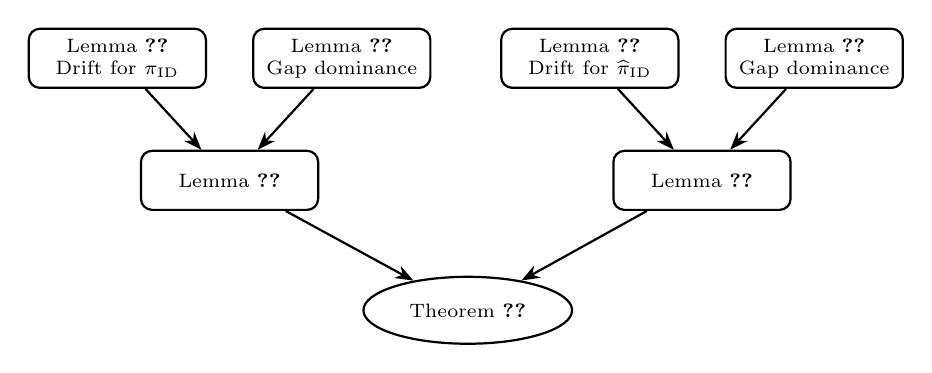
\begin{tikzpicture}[
  lemma/.style={draw, rounded corners, minimum width=2.25cm, minimum height=0.75cm, align=center, font=\scriptsize},
  theorem/.style={draw, ellipse, minimum width=2.65cm, minimum height=0.85cm, align=center, font=\scriptsize},
  >=Stealth, thick
]
\node[lemma] (l7) at (0,0) {Lemma~\ref{lem:lemma5-zhang2025}\\Drift for $\piid$};
\node[lemma] (l8) at (2.85,0) {Lemma~\ref{lem:simu-lemma-hete}\\Gap dominance};
\node[lemma] (l1) at (1.425,-1.55) {Lemma~\ref{lem:rhorel-rhohpiid-hete}};
\node[lemma] (l11) at (6.0,0) {Lemma~\ref{lem:DC-Vhat-hete}\\Drift for $\pihid$};
\node[lemma] (l12) at (8.85,0) {Lemma~\ref{lem:simu-lemma-hat-hete}\\Gap dominance};
\node[lemma] (l2) at (7.425,-1.55) {Lemma~\ref{lem:rhohrel-rhopihid-hete}};
\node[theorem] (thm1) at (4.45,-3.2) {Theorem~\ref{thm-heteWCMDP}};
\draw[->] (l7) -- (l1);
\draw[->] (l8) -- (l1);
\draw[->] (l11) -- (l2);
\draw[->] (l12) -- (l2);
\draw[->] (l1) -- (thm1);
\draw[->] (l2) -- (thm1);
\end{tikzpicture}
\caption{Flowchart for the proof of Theorem~\ref{thm-heteWCMDP}. We omit auxiliary model-accuracy lemmas.}
\label{fig:flow-pf-thmhete}
\end{figure}

\paragraph{Model accuracy.} In order to get the final result, we firstly show the model accuracy lemmas we used, whose proofs are deferred to Appendix~\ref{subsec:model-accuracy}. We begin with a standard concentration bound for the empirical estimate of each single-armed transition kernel.
The next lemma gives a uniform $\ell_1$ bound over all arms $i\in[N]$ and all state-action pairs $(s,a)\in\States\times\Actions$.
\begin{lemma}\label{samplesize-singlearm_accu}
    Fix $\eta \in (0,1)$. With probability at least $1 - \eta$, we have
    \begin{align*}
        \max_{i\in[N]}\max_{s \in \mathcal{S}, a \in \mathcal{A}} \onenorm{P_i(\cdot\mid s,a) - \widehat{P}_i(\cdot\mid s,a)} \leq \sqrt{\frac{2S \log(2) + 2\log (SAN/\eta)}{n}}.
    \end{align*}
\end{lemma}
We next lift the single-armed model accuracy bound to the \(N\)-armed
system. The error accumulates across arms, which leads to an additional
factor of \(N\). The same bound also holds for the transition matrices
induced by any fixed policy.

\begin{lemma}
\label{lem:lift-single-to-Narm}
Suppose that we have the following uniform single-armed model accuracy bound: 
\[
    \max_{i\in[N]}\max_{s\in\States,a\in\Actions}
    \onenorm{P_i(\cdot\mid s,a)-\widehat P_i(\cdot\mid s,a)}
    \le
    \delta .
\]
Then the $N$-armed model accuracy satisfies
\[
    \max_{\bms\in\States^N,\bma\in\Actions^N}
    \onenorm{\bp(\cdot\mid\bms,\bma)-\bphat(\cdot\mid\bms,\bma)}
    \le
    N\delta .
\]
Moreover, for any policy \(\pi\), the induced transition matrices
\[
    \bp^\pi(\bms,\bms')
    =
    \sum_{\bma\in\Actions^N}
    \pi(\bma\mid\bms)\bp(\bms'\mid\bms,\bma),
    \qquad
    \bphat^\pi(\bms,\bms')
    =
    \sum_{\bma\in\Actions^N}
    \pi(\bma\mid\bms)\bphat(\bms'\mid\bms,\bma)
\]
satisfy
\(
    \infinfnorm{\bp^\pi-\bphat^\pi}
    \le
    N\delta .
\)
\end{lemma}

We now state the two Lemma~\ref{lem:rhorel-rhohpiid-hete} and Lemma~\ref{lem:rhohrel-rhopihid-hete}.
\begin{lemma}\label{lem:rhorel-rhohpiid-hete}
Consider an $N$-armed WCMDP satisfying
Assumption~\ref{ass:unichain-unifmixing}. Suppose that the empirical system $\{\widehat{P}_i\}_{i\in[N]}$ satisfies 
\[
\max_{i\in[N]}\max_{s \in \mathcal{S},a \in \mathcal{A}} \left\| \widehat{P}_i(\cdot \mid s, a) - P_i(\cdot \mid s, a) \right\|_1 \le \delta.
\]
Then for the ID policy computed from the true system $\{{P}_i\}_{i\in[N]}$, $\piid,$ we have
    \[\rhorel - \rhohat^{\piid}(\bms_0)\le \frac{3(2r_{\max}+L_h)}{\rho_V}N\delta+\left[\frac{(2r_{\max}+L_h)K_V}{L_h\rho_V}+2 r_{\max}K_{\mathrm{conf}}\right]\frac{1}{\sqrt{N}},\]
where $L_h$ is a constant defined in~\eqref{eq:def-Lh-Ctau-tau} and $\rho_V, K_{\mathrm{conf}}$ are constants defined in~\eqref{eq:cons-hetero-drift}.   
\end{lemma}
\begin{lemma}\label{lem:rhohrel-rhopihid-hete}
Consider an $N$-armed WCMDP  satisfying
Assumption~\ref{ass:unichain-unifmixing}. Suppose that the empirical system $\{\widehat{P}_i\}_{i\in[N]}$ satisfies
\[
\max_{i\in[N]}\max_{s \in \mathcal{S},\ a \in \mathcal{A}} \left\| \widehat{P}_i(\cdot \mid s, a) - P_i(\cdot \mid s, a) \right\|_1 \le \delta\le\frac{1}{4S\tmix(5+\log_2S)}.
\]
Then for the ID policy computed from the empirical system $\{\widehat{P}_i\}_{i\in[N]}$, $\pihid,$ we have
    \[\rhohrel - \rho^{\pihid}(\bms_0)\le \frac{3(2r_{\max}+L_h)}{\rho_V}N\delta+\left[\frac{(2r_{\max}+L_h)K_V}{L_h\rho_V}+2 r_{\max}K_{\mathrm{conf}}\right]\frac{1}{\sqrt{N}},\]
where $\tmix$ is defined in Assumption~\ref{ass:unichain-unifmixing}, $L_h$ is defined in~\eqref{eq:def-Lh-Ctau-tau} and $\rho_V, K_{\mathrm{conf}}$ are defined in~\eqref{eq:cons-hetero-drift}.
\end{lemma}

Here we provide the proof of Lemma~\ref{lem:rhorel-rhohpiid-hete} to illustrate how our Lyapunov framework is applied; the proof of Lemma~\ref{lem:rhohrel-rhopihid-hete} is deferred to the Appendix~\ref{subsec:pr-C2-hete}.
\paragraph{Proof of Lemma~\ref{lem:rhorel-rhohpiid-hete}}

We leverage the Lyapunov function $V$ constructed in~\citet{zhang2025projection} for analyzing the optimality gap of the ID policy in WCMDP. {In particular, the function $V$ is defined in \eqref{def:lya-true} with respect to the one-hot representation of the system state $\bm{S}_t$, denoted as $\bm{X}_t.$ Specifically, \(X_{i,t} = (X_{i,t}(s))_{s\in\mathbb{S}} \in \mathbb{R}^{S}\), 
where \(X_{i,t}(s)=1\) if \(S_{i,t}=s\) and \(0\) otherwise.} 

\paragraph{Step 1: Lyapunov analysis} 
We show that the Lyapunov function $V$ satisfies \ref{cond:drift} and \ref{cond:dominance} in our framework, stated formally as Lemma~\ref{lem:lemma5-zhang2025} and Lemma~\ref{lem:simu-lemma-hete}, respectively. 

\begin{lemma}[{\citealt[Lemma 5]{zhang2025projection}}]\label{lem:lemma5-zhang2025}
    Consider any $N$-armed WCMDP and assume that it satisfies Assumption~\ref{ass:unichain-unifmixing}. The Lyapunov function $V$ defined in (\ref{def:lya-true}) satisfies
\begin{equation}\label{drift_cond_heterogenous}
    \mathbb{E}^{\piid}[V(\bm{X}_{t+1})-V(\bm{X}_t)|\bm{X}_t=\bmx]\le -\rho_VV(\bmx)+K_V/\sqrt{N},
\end{equation}
where 
\begin{equation}\label{eq:cons-hetero-drift}
    \begin{gathered}
        \rho_V = \frac{(1 - \gamma)}{1 + \frac{L_h}{\eta_c}}, \;\;
        \eta_c = \min \left\{ \frac{\alpha_{\min}}{3},\ 
\frac{\alpha_{\min}}{4} \cdot \left( \left\lceil \frac{(4c_{\max} - \alpha_{\min})K}{\alpha_{\min}} \right\rceil \right)^{-1} \right\}, \;\;
\alpha_{\min}=\min_{k\in[K]}\alpha_k, \\
K_V = 2C_h + C_h K_{\mathrm{conf}} + 2L_h K_{\mathrm{mono}} + \rho_V L_h K_{\mathrm{cov}}, \;\;
C_h=2C_\tau(Kc_{\max}+r_{\max}),\\
K_{\mathrm{conf}}=\frac{2Kc_{\max}+M_c}{\eta_c}, \;\;
K_{\mathrm{mono}}=\frac{(2+K_{\mathrm{conf}})C_h+M_c}{\eta_c}, \;\;
K_{\mathrm{cov}}=\frac{\eta_c+M_c+L_h}{\eta_c}, \;\;
M_c = \frac{\alpha_{\min}}{2}.
    \end{gathered}
\end{equation}
Here $\gamma$ is defined in~\eqref{def:gamma-tau-g} and $L_h, C_\tau$ are defined in~\eqref{eq:def-Lh-Ctau-tau}.
\end{lemma}
All constants above depend on the MDP parameters only through the mixing-time upper bound $\tmix$.

\begin{lemma}\label{lem:simu-lemma-hete}
    For each system state $\bms$, denote $A_i^{\piid}$ as the action applied to arm $i$ under policy $\piid$. Define
    $
    r^{\piid}(\bms)=\frac{1}{N}\sum_{i=1}^N\E[r_i(s_i,A_i^{\piid})].
    $
    Then
    \[
    \rhorel-r^{\piid}(\bms)\le \frac{2r_{\max}+L_h}{L_h}V(\bmx)+\frac{2r_{\max}K_{\mathrm{conf}}}{\sqrt{N}}.
    \]
\end{lemma}
The proof of Lemma~\ref{lem:simu-lemma-hete} follows the same argument as \citet[Lemma~4]{zhang2025projection}; we omit it here.



That is, our Lyapunov function $V$ satisfies \ref{cond:drift} and \ref{cond:dominance} with $F(\bmx)=V(\bmx),$ $G_1(N)=K_V/\sqrt{N}$ and $G_2(N)={2r_{\max}K_{\mathrm{conf}}}/{\sqrt{N}}$.%

\paragraph{Step 2: Drift transfer.} 
The following lemma formalizes this drift-transfer step in a reusable
form. In the lemma, \(Q\) denotes the transition matrix under which the
Lyapunov drift inequality is available, while \(P\) denotes the transition
matrix under which the long-run performance is evaluated. The proof is a
finite-horizon telescoping argument and is given in
Appendix~\ref{sec:common-technical-lemmas}.
\begin{lemma}
\label{lem:generic-drift-transfer}
Let \(P\) and \(Q\) be two transition matrices on the same finite state
space \(\mathcal Z\). Let \(\bar r:\mathcal Z\to\mathbb R\) be a bounded reward function. For any initial state \(z_0\), define the
long-run average reward under \(P\) by
\[
    \rho_P(z_0)
    :=
    \lim_{T\to\infty}
    \frac1T
    \sum_{t=0}^{T-1}
    \mathbb E_P[\bar r(Z_t)\mid Z_0=z_0].
\]
Since \(\mathcal Z\) is finite, the Cesaro average defining
\(\rho_P(z_0)\) exists for every initial state \(z_0\), although
\(P^t(z_0,\cdot)\) need not converge. Suppose there exist functions
\(V:\mathcal Z\to\mathbb R\) and \(F:\mathcal Z\to\mathbb R_+\),
constants \(C_0>0\) and \(C_0'\ge0\), two nonnegative terms
\(G_1(N),G_2(N)\), and a scalar benchmark \(R\), such that, for every
\(z\in\mathcal Z\),
\[
    [(Q-I)V](z)
    \le
    -C_0F(z)+G_1(N),
    \qquad
    R-\bar r(z)
    \le
    C_0'F(z)+G_2(N).
\]
Then, for every initial state \(z_0\),
\[
    R-\rho_P(z_0)
    \le
    \frac{C_0'}{C_0}G_1(N)
    +
    G_2(N)
    +
    \frac{C_0'}{C_0}
    \sup_{z\in\mathcal Z}
    \left|[(P-Q)V](z)\right|.
\]
In particular, the conclusion does not require the distribution of \(Z_t\)
under \(P\) to converge as \(t\to\infty\).
\end{lemma}


We now apply Lemma~\ref{lem:generic-drift-transfer} with
\(
    Q=\bp^{\piid},
    P=\bphat^{\piid},
    R=\rhorel,
    F=V,
    \bar r=r^{\piid}.
\)
Lemmas~\ref{lem:lemma5-zhang2025} and~\ref{lem:simu-lemma-hete} give the
required drift and dominance inequalities with
\[
    C_0=\rho_V,
    \qquad
    C_0'=\frac{2r_{\max}+L_h}{L_h},
    \qquad
    G_1(N)=\frac{K_V}{\sqrt N},
    \qquad
    G_2(N)=\frac{2r_{\max}K_{\mathrm{conf}}}{\sqrt N}.
\]
Hence,
\[
\begin{aligned}
    \rhorel-\widehat\rho^{\piid}(\bms_0)
    \le
    \frac{2r_{\max}+L_h}{L_h\rho_V}
    \sup_{\bmx}
    \left|
    (\bphat^{\piid}-\bp^{\piid})V(\bmx)
    \right|  +
    \left[
    \frac{(2r_{\max}+L_h)K_V}{L_h\rho_V}
    +
    2r_{\max}K_{\mathrm{conf}}
    \right]\frac1{\sqrt N}.
\end{aligned}
\]
By Lemma~\ref{lem:lift-single-to-Narm},
\(
    \infinfnorm{\bphat^{\piid}-\bp^{\piid}}
    \le
    N\delta .
\)
Moreover, \(\|V\|_\infty\le L_h\) according to \eqref{eq:bound-V-hete}. Therefore,
\[
\begin{aligned}
    \sup_{\bmx}
    \left|
    (\bphat^{\piid}-\bp^{\piid})V(\bmx)
    \right|
    \le
    \infinfnorm{\bphat^{\piid}-\bp^{\piid}}\|V\|_\infty 
    \le
    L_hN\delta .
\end{aligned}
\]
Substituting this bound gives the desired result.

\paragraph{Completing the proof of Theorem~\ref{thm-heteWCMDP}}\label{subsec:final-pr-thm1}
To combine Lemma~\ref{lem:rhorel-rhohpiid-hete} and Lemma~\ref{lem:rhohrel-rhopihid-hete} to obtain Theorem~\ref{thm-heteWCMDP}, what is left to do is to connect the single-armed model accuracy $\delta$ to the number of samples $n$. 
First, we notice that when
$
n\le\left(2S\log2+2\log(SAN/\eta)\right)16\tau^2S^2(5+\log_2S)^2,
$
we can choose $C_1=8\tau(5+\log_2S)$ so that
\[
    \rho^\star(\bms_0)-\rho^{\pihid}(\bms_0)\le 1\le C_1N\sqrt{\frac{S + \log (SAN/\eta)}{n}}+\frac{C_2}{\sqrt{N}} .
\]
Therefore, we only need to consider the case where
$n\ge\left(2S\log2+2\log(SAN/\eta)\right)16\tau^2S^2(5+\log_2S)^2.$
In this case, according to Lemma \ref{samplesize-singlearm_accu}, we have the single-armed model accuracy:
\[
\max_{i\in [N]}\max_{s \in \mathcal{S},\ a \in \mathcal{A}} \left\| \widehat{P}_i(\cdot \mid s, a) - P_i(\cdot \mid s, a) \right\|_1 \le \delta\triangleq \sqrt{\frac{2S \log(2) + 2\log (SAN/\eta)}{n}}\le\frac{1}{4\tau S(5+\log_2S)}.
\]
with probability at least $1-\eta$. In this case, the conditions of Lemma~\ref{lem:rhorel-rhohpiid-hete} and Lemma~\ref{lem:rhohrel-rhopihid-hete} are satisfied. It is straightforward to combine the results of these two lemmas, plus the fact that the reward from each arm is upper bounded by $r_{\max}$, to get Theorem~\ref{thm-heteWCMDP}.

\section{Proof of Theorem~\ref{thm-homoRB}}
\label{sec:proof_outline_thm_RB}

We use the framework in Section~\ref{sec:Lyapunov-Framework} to prove
Theorem~\ref{thm-homoRB}. The proof follows the same decomposition
as in~\eqref{eq:decomp}. It is sufficient to bound
\(\rho^{\mathrm{rel}}-\widehat\rho^{\pits}(\bms_0)\) and
\(\widehat\rho^{\mathrm{rel}}-\rho^{\pihts}(\bms_0)\).

\paragraph{Proof roadmap.} The proof has two main intermediate bounds. First, we bound
\(\rho^{\mathrm{rel}}-\widehat\rho^{\pits}(\bms_0)\). Here the two-set
policy is computed from the true model but is evaluated
under the empirical model. We use the Lyapunov drift bound for the two-set
policy (Lemma~\ref{lem:DC-RB}) and the gap-dominance bound
(Lemma~\ref{lem:C2-RB}). These two lemmas correspond to
Conditions~\ref{cond:drift} and~\ref{cond:dominance} in our Lyapunov
framework. Together with the drift-transfer argument, they imply
Lemma~\ref{lem:rhorel-rhohpi-homo}.

Second, we bound
\(\widehat\rho^{\mathrm{rel}}-\rho^{\pihts}(\bms_0)\). Here the two-set
policy is computed from the empirical model and evaluated under the true
model. This part uses the same Lyapunov argument, but but it also uses
Theorem~\ref{thm:LP_perturbation_main_complete} to justify the empirical Lyapunov analysis. Then the empirical drift condition
(Lemma~\ref{lem:DC-Vhat-homo}) and the empirical gap dominance bound
(Lemma~\ref{lem:C2-hat-RB}) imply
Lemma~\ref{lem:rhohrel-rhopihat-homo}.

Both intermediate lemmas use model-accuracy lemma, which we state below.
Figure~\ref{fig:flow-pf-thmhomo} summarizes the main steps.
\begin{figure}[htbp]
\centering
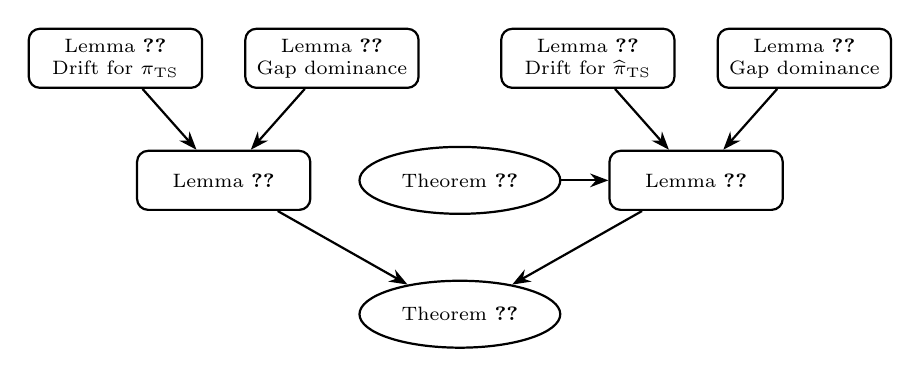
\begin{tikzpicture}[
  lemma/.style={draw, rounded corners, minimum width=2.2cm, minimum height=0.75cm, align=center, font=\scriptsize},
  theorem/.style={draw, ellipse, minimum width=2.55cm, minimum height=0.85cm, align=center, font=\scriptsize},
  >=Stealth, thick
]
\node[lemma] (dc) at (0,0) {Lemma~\ref{lem:DC-RB}\\Drift for $\pits$};
\node[lemma] (c2) at (2.75,0) {Lemma~\ref{lem:C2-RB}\\Gap dominance};
\node[lemma] (l30) at (1.375,-1.55) {Lemma~\ref{lem:rhorel-rhohpi-homo}};
\node[lemma] (dchat) at (6.0,0) {Lemma~\ref{lem:DC-Vhat-homo}\\Drift for $\pihts$};
\node[lemma] (c2hat) at (8.75,0) {Lemma~\ref{lem:C2-hat-RB}\\Gap dominance};
\node[lemma] (l33) at (7.375,-1.55) {Lemma~\ref{lem:rhohrel-rhopihat-homo}};
\node[theorem] (pert) at (4.375,-1.55) {Theorem~\ref{thm:LP_perturbation_main_complete}};
\node[theorem] (thm) at (4.375,-3.25) {Theorem~\ref{thm-homoRB}};
\draw[->] (dc) -- (l30);
\draw[->] (c2) -- (l30);
\draw[->] (dchat) -- (l33);
\draw[->] (c2hat) -- (l33);
\draw[->] (pert) -- (l33);
\draw[->] (l30) -- (thm);
\draw[->] (l33) -- (thm);
\end{tikzpicture}
\caption{Flowchart for the proof of Theorem~\ref{thm-homoRB}. We omit auxiliary model-accuracy lemmas.}
\label{fig:flow-pf-thmhomo}
\end{figure}

\paragraph{Model accuracy.} The model-accuracy lemma used for the homogeneous RB setting is a special
case of the corresponding lemmas for the heterogeneous WCMDP setting. We state it below.
\begin{lemma}\label{samplesize-singlearm_accu_rb}\label{single-to-Narm-accu}
Fix $\eta\in(0,1)$. With probability at least $1-\eta$,
\[
    \max_{s\in\States,a\in\Actions}
    \onenorm{P(\cdot\mid s,a)-\widehat P(\cdot\mid s,a)}
    \le
    \sqrt{\frac{2S\log(2)+2\log(SA/\eta)}{n}}.
\]
Moreover, if the left-hand side is at most $\delta$, then the induced $N$-armed kernels satisfy
\[
    \max_{\bms\in\States^N,\bma\in\Actions^N}
    \onenorm{\bp(\cdot\mid\bms,\bma)-\bphat(\cdot\mid\bms,\bma)}
    \le N\delta.
\]
And for any policy \(\pi\), the induced transition matrices $\bp^\pi, \bphat^\pi$ satisfy $\infinfnorm{\bp^\pi-\bphat^\pi}
    \le
    N\delta .$

\end{lemma}
We now state Lemma~\ref{lem:rhorel-rhohpi-homo} and Lemma~\ref{lem:rhohrel-rhopihat-homo}.
\begin{lemma}[Bound on $\rho^{\mathrm{rel}}-\widehat\rho^{\pits}(\bms_0)$]\label{lem:rhorel-rhohpi-homo}
Consider an $N$-armed RB problem with an initial state $\bms_0$ satisfying Assumptions~\ref{ass:RB} and~\ref{ass:strict_action_gaps}. Suppose
\(
N\ge \max\left\{\frac{4}{\min\{y^\star(\tilde{s},0),y^\star(\tilde{s},1)\}},\left(\frac{4M}{\gamma}\right)^2\right\}
\)
and the single-armed model accuracy satisfies
\[
\max_{s\in\mathcal S,\ a\in\mathcal A}\left\|\widehat P(\cdot\mid s,a)-P(\cdot\mid s,a)\right\|_1\le \delta,
\]
where $\gamma$ is defined in~\eqref{eq:def-beta-Q-b-bareta-gamma} and $M$ is defined in~\eqref{def:g-C-M}. Then
\[
\rho^{\mathrm{rel}}-\widehat\rho^{\pits}(\bms_0)
\le C_6N\delta+6\exp(8)S\widetilde V_{\max}\exp(-CN),
\]
where $\widetilde V_{\max}$ is defined in~\eqref{eq:def-Vtilde_max}, and $C_6,C$ are constants independent of $N$.
\end{lemma}

\begin{lemma}[Bound on $\widehat\rho^{\mathrm{rel}}-\rho^{\pihts}(\bms_0)$]\label{lem:rhohrel-rhopihat-homo}
Consider an $N$-armed RB problem with an initial state $\bms_0$ satisfying Assumptions~\ref{ass:RB} and~\ref{ass:strict_action_gaps}. Suppose
\(
N\ge \max\left\{\frac{4}{\min\{y^\star(\tilde{s},0),y^\star(\tilde{s},1)\}},\left(\frac{4\widehat M^{\mathrm{up}}}{\widehat\gamma^{\mathrm{low}}}\right)^2\right\}
\)
and the single-armed model accuracy satisfies
\[
\max_{s\in\mathcal S,\ a\in\mathcal A}\left\|\widehat P(\cdot\mid s,a)-P(\cdot\mid s,a)\right\|_1
\le \delta\le \delta_{\min},
\]
where $\widehat M^{\mathrm{up}}$ is defined in~\eqref{def:ubmhat}, $\widehat\gamma^{\mathrm{low}}$ is defined in~\eqref{eq:def-lbg-upg-ubKvh}, and $\delta_{\min}$ is defined in~\eqref{eq:def-delta-min}. Then
\[
\widehat\rho^{\mathrm{rel}}-\rho^{\pihts}(\bms_0)
\le C_7N\delta+6\exp(8)S\widehat{\widetilde V}_{\max}\exp(-\widehat C N),
\]
where $\widehat{\widetilde V}_{\max}$ is defined in~\eqref{def:hat-tilde-V-max}, and $C_7,\widehat C$ are constants independent of $N$.
\end{lemma}

Lemma~\ref{lem:rhorel-rhohpi-homo} is proved in Appendix~\ref{subsec:pr-C1-homo}. Here we provide a proof outline of Lemma~\ref{lem:rhohrel-rhopihat-homo},
which is the part where the perturbation analysis enters the proof of
Theorem~\ref{thm-homoRB}. The complete proof is deferred to
Appendix~\ref{subsec:pr-C2-homo}. Unlike
Lemma~\ref{lem:rhorel-rhohpi-homo}, which analyzes the true two-set policy,
Lemma~\ref{lem:rhohrel-rhopihat-homo} analyzes the learned two-set policy
\(\pihts\) under the true model. Therefore, before applying the Lyapunov
framework, we must first verify that the empirical LP solution preserves
the structural properties required by the two-set policy and its Lyapunov
analysis. We use Theorem~\ref{thm:LP_perturbation_main_complete} exactly for this purpose.
\paragraph{Proof outline of Lemma~\ref{lem:rhohrel-rhopihat-homo}.}

\paragraph{Step 1: Structural stability from the perturbation theorem.} Since the single-armed model accuracy satisfies the requirements of Theorem~\ref{thm:LP_perturbation_main_complete}, the empirical LP
preserves the key structure of the true LP. Therefore, the empirical two-set objects used below,
including \(\widehat g\) and \(\widehat V\), are well-defined.

\paragraph{Step 2: Empirical Lyapunov analysis.}
We now apply the two-set Lyapunov analysis to the empirical system. Let
\(
    \Sigma_t
    =
    (\bm X_t,D_t^{\mathrm{OL}},D_t^{\pihbst})
\)
denote the augmented state of the learned two-set policy, and let
\(\widehat V\) be the empirical Lyapunov function constructed from
\(\widehat y^\star\), \(\widehat\mu^\star\), and the perturbed local
stability matrix $\phihat$. The empirical two-set policy admits the following drift and
gap-dominance bounds, stated formally as
Lemmas~\ref{lem:DC-Vhat-homo} and~\ref{lem:C2-hat-RB},
respectively. Informally, for every augmented state \(\sigma\),
\[
    (\bphat^{\pihts}-I)\widehat V(\sigma)
    \le
    -\frac{\widehat\gamma}
    {4(\widehat\beta+r_{\max})}
    \widehat g(\sigma)
    +
    6\exp(8)S\widehat{\widetilde V}_{\max}
    \exp(-\widehat C N),
\]
and
\(
    \widehat\rho^{\mathrm{rel}}-r^{\pihts}(\sigma)
    \le
    \widehat g(\sigma).
\)
Thus, in the notation of the Lyapunov framework, the empirical Lyapunov
function \(\widehat V\) satisfies Conditions~\ref{cond:drift}
and~\ref{cond:dominance} with
\(
    F(\sigma)=\widehat g(\sigma),
    C_0=\frac{\widehat\gamma}{4(\widehat\beta+r_{\max})},
    G_1(N)=6\exp(8)S\widehat{\widetilde V}_{\max}\exp(-\widehat C N),
    C_0'=1,
    G_2(N)=0.
\)
The perturbation theorem is used here to ensure that the hatted objects
appearing in these bounds are well-defined and that the empirical
constants are uniformly controlled.

\paragraph{Step 3: Drift transfer.}
The drift bound in Step 2 is for the empirical transition kernel
\(\bphat^{\pihts}\), while Lemma~\ref{lem:rhohrel-rhopihat-homo} concerns
the performance of \(\pihts\) under the true transition kernel
\(\bp^{\pihts}\). We therefore apply
Lemma~\ref{lem:generic-drift-transfer} with
\(
    Q=\bphat^{\pihts},
    P=\bp^{\pihts},
    R=\widehat\rho^{\mathrm{rel}},
    F=\widehat g,
    V=\widehat V,
    \bar r=r^{\pihts}.
\)
Using the values of \(C_0,C_0',G_1(N),G_2(N)\) from Step 2, we obtain
\[
\begin{aligned}
    \widehat\rho^{\mathrm{rel}}
    -
    \rho^{\pihts}(\bms_0)
    \le&
    \frac{4(\widehat\beta+r_{\max})}{\widehat\gamma}
    \sup_{\sigma}
    \left|
    (\bp^{\pihts}-\bphat^{\pihts})
    \widehat V(\sigma)
    \right|  +
    \frac{4(\widehat\beta+r_{\max})}{\widehat\gamma}
    6\exp(8)S\widehat{\widetilde V}_{\max}
    \exp(-\widehat C N).
\end{aligned}
\]
The model-error term is upper bounded by Lemma~\ref{lem:p-phat-vhat}:
\(
    \sup_{\sigma}
    \left|
    (\bp^{\pihts}-\bphat^{\pihts})
    \widehat V(\sigma)
    \right|
    \le
    \widehat V_{\max}N\delta.
\)
Substituting this bound into the display from Step 3 gives
\[
\begin{aligned}
    \widehat\rho^{\mathrm{rel}}
    -
    \rho^{\pihts}(\bms_0)
    \le&
    \frac{4\widehat V_{\max}(\widehat\beta+r_{\max})}
    {\widehat\gamma}
    N\delta  +
    \frac{4(\widehat\beta+r_{\max})}{\widehat\gamma}
    6\exp(8)S\widehat{\widetilde V}_{\max}
    \exp(-\widehat C N).
\end{aligned}
\]

\paragraph{Step 4: Replacing empirical constants by deterministic bounds.}
Finally, Theorem~\ref{thm:LP_perturbation_main_complete} and the auxiliary well-definedness
lemmas provide deterministic bounds on the empirical constants:
\(
    \widehat\gamma\ge \widehat\gamma^{\mathrm{low}},
    \widehat\beta\le \widehat\beta^{\max},
    \|\widehat V\|_\infty\le \widehat V_{\max},
    \widehat{\widetilde V}_{\max}<\infty.
\)
These bounds depend only on the original single-armed RB parameters, not on
\(N,n,\eta\), or the initial state. Hence the previous display implies
\[
    \widehat\rho^{\mathrm{rel}}
    -
    \rho^{\pihts}(\bms_0)
    \le
    C_7N\delta
    +
    6\exp(8)S\widehat{\widetilde V}_{\max}
    \exp(-\widehat C N),
\]
for a constant \(C_7\) independent of \(N,n,\eta\), and \(\bms_0\). This
is Lemma~\ref{lem:rhohrel-rhopihat-homo}.
\paragraph{Completing the proof of Theorem~\ref{thm-homoRB}.}
Combining Lemma~\ref{lem:rhorel-rhohpi-homo} and Lemma~\ref{lem:rhohrel-rhopihat-homo} yields Theorem~\ref{thm-homoRB} once we relate the single-armed model accuracy parameter $\delta$ to the sample size $n$ under the generative model.
First, we notice that when
$n\le\left(2S\log2+2\log(SA/\eta)\right)/\delta_{\min}^2,
$
where $\delta_{\min}$ is defined in~\eqref{eq:def-delta-min}, we can choose $C'=2/\delta_{\min}$, then 
\[
    \rho^\star(\bms_0)-\rho^{\pihts}(\bms_0)\le 1\le C'N\sqrt{\frac{S + \log (SA/\eta)}{n}}+C''\exp(-C_5N).
\]
Therefore, we only need to consider the case when
$
n\ge\left(2S\log2+2\log(SA/\eta)\right)/\delta_{\min}^2,
$
In this case, according to Lemma \ref{samplesize-singlearm_accu}, we have the single-armed model accuracy:
\[
    \max_{s \in \mathcal{S},\ a \in \mathcal{A}} \left\| \widehat{P}(\cdot \mid s, a) - P(\cdot \mid s, a) \right\|_1 \le \delta\triangleq \sqrt{\frac{2S \log(2) + 2\log (SA/\eta)}{n}}\le\delta_{\min},
\]
with probability at least $1-\eta$. We consider the case when
\begin{equation}\label{eq:def-Nmax}
    N\ge N_{\max}\triangleq\max\left\{\frac{4}{\min\{y^\star(\tilde{s},0),y^\star(\tilde{s},1)\}},\left(\frac{4M}{\gamma}\right)^2,\left(\frac{4\ubmhat}{\lbgmhat}\right)^2\right\},
\end{equation}
where $M$ is defined in \eqref{def:g-C-M}, $\gamma$ in~\eqref{eq:def-beta-Q-b-bareta-gamma}, $\ubmhat$ in \eqref{def:ubmhat} and $\lbgmhat$ in \eqref{eq:def-lbg-upg-ubKvh}. Based on these conditions, both the conditions of $N$ and $\delta$ in Lemmas~\ref{lem:rhorel-rhohpi-homo} and~\ref{lem:rhohrel-rhopihat-homo} hold. Therefore, we can combine the results of these two lemmas by choosing 
$
    C_3=C_6+C_7,
    C_4=6\exp(8)S(\tilde{V}_{\max}+\widehat{\tilde{V}}_{\max})
    \text{ and }
    C_5=\min\{C,\widehat C\},
$               
which completes the proof.

\section{Proof of Theorem~\ref{thm:LP_perturbation_main_complete}}\label{sec:proof-lp-pa}

In this section we provide the proof of Theorem \ref{thm:LP_perturbation_main_complete}, which will be preceded by many intermediate lemmas, organized into three subsections \ref{sec:pert_subsec_1}, \ref{sec:pert_subsec_2}, \ref{sec:pert_subsec_3} and \ref{subsec:final-pr-perturbation-full}. We firstly give a proof outline in \ref{sec:pr-outline-pert} to show the high-level ideas.

\subsection{Proof outline}\label{sec:pr-outline-pert}
The proof uses a primal-dual perturbation argument. Under the
nondegeneracy and strict-gap assumptions, a small perturbation of the
transition kernel should not change which LP constraints are active. We
therefore build candidate primal and dual solutions for the perturbed LP
using the same active structure as in the true LP. We then check primal
feasibility, dual feasibility, complementary slackness, and uniqueness.

One complication is that the RB LP has a redundant flow-balance constraint,
and the dual bias vector is only unique up to an additive constant. For
this reason, we first perturb the state occupancy instead of perturbing
the primal and dual variables directly. Around the optimal state occupancy
\(\mu^\star\), the locally linear policy follows \(\pibst\) at all
non-neutral states and uses the neutral state \(\tilde s\) to satisfy the
budget. This gives the local linearization matrix
\(U=P^{\pibst}-(c^{\pibst}-\alpha\one)\xi\), where
\(\xi=P_{\tilde s1}-P_{\tilde s0}\). Replacing \(P\) by \(\Phat\) gives
the perturbed matrix \(\uhat\).

We define \(H_U=(I-\Phi)^{-1}-\one\mu^\star\) and
\(
    \muhat
    =
    \mu^\star\bigl(I-(\uhat-U)H_U\bigr)^{-1}.
\)
The matrix \(H_U\) measures how sensitive the state occupancy is to the
model perturbation. The key identity is
\(
    \muhat-\mu^\star=\muhat(\uhat-U)H_U.
\)
This is similar to the usual perturbation formula for stationary
distributions of Markov chains, although \(U\) and \(\uhat\) are not
transition matrices.

After constructing \(\muhat\), we use a linear map \(W\) to define the
primal candidate \(\yhat=\muhat W\). The construction of \(W\) ensures that
\(\yhat\) satisfies the perturbed budget, flow-balance, and normalization
constraints. It also preserves the support pattern: active entries of
\(y^\star\) remain positive, while inactive entries remain zero.
For the dual side, we construct \((\zetahat,\lambdahat,\hhat)\) so that
the perturbed dual constraints are tight on the active state-action pairs.
The dual perturbation bounds then show that inactive constraints still
have positive slack. Thus the constructed primal and dual candidates are
feasible and satisfy complementary slackness, so they are optimal. The
strict slack on inactive actions also gives uniqueness and support
preservation.

Finally, support preservation implies that the empirical optimal
single-arm policy can differ from the true one only at the neutral state.
Together with a Markov-chain perturbation bound, this gives the
aperiodicity, irreducibility, and mixing-time conclusion in the theorem.
\subsection{Candidate state occupancy construction}
\label{sec:pert_subsec_1}
Throughout the proof, fix an arbitrary policy $\pistar$ which satisfies that $ \pistar(s)=\pibst(s)$ for all $ s \neq \Tilde{s}$. It is straightforward to check that
$
    P^{\pibst} - (c^{\pibst} -\alpha \one)\xi = P^{\pistar} - (c^{\pistar} -\alpha \one)\xi
$
where for any policy $\pi$, $c^{\pi}(s) = \pi(1 \mid s)$, and $\xi$ is the row vector $P_{\tilde{s}1}-P_{\tilde{s}0}$. We then define the local linearization matrix $U$ and its perturbed analogue
\begin{align*}
    U = P^{\pistar} - (c^{\pistar} -\alpha \one)\xi, 
    \qquad
    \uhat = \Phat^{\pistar} - (c^{\pistar} -\alpha \one)\widehat \xi,
\end{align*}
where $\xihat \triangleq \Phat_{\tilde{s}1}-\Phat_{\tilde{s}0}$. We also define $H_U = (I - (U - \one \mu^\star))^{-1} - \one \mu^\star.$ 
Note that $U-\one \mu^\star=\Phi$, so the inverse $(I - (U - \one \mu^\star))^{-1}$ exists due to the local stability condition of Assumption~\ref{ass:RB}.
Finally we define the candidate state occupancy distribution
\begin{equation}
    \muhat\triangleq \mu^\star (I - (\uhat-U)H_U)^{-1}.
    \label{eq:muhat-definition}
\end{equation} 
Such a definition requires the invertibility of $(I - (\uhat-U)H_U)^{-1}$, so it suffices for now to require that we have $\ltwonorm{(\uhat-U)H_U}< 1$.
This definition is motivated by the stationary distribution perturbation identity for Markov chains \citep{meyer_jr_role_1975} and we can now verify that an analogous identity holds in our case:
\begin{lemma}
    \label{lem:pert_analysis_sim_lemma}
    Suppose $(I - (U - \one \mu))$ and $(I - (\uhat-U)H_U)$ are both invertible. Then
    $
        \muhat - \mu^\star = \muhat (\uhat - U)H_U.
    $
\end{lemma}
\begin{proof}{Proof}
    Right-multiplying both sides of~\eqref{eq:muhat-definition} by $(I - (\uhat-U)H_U)$, we have that
    $
        \mu^\star = \muhat (I - (\uhat-U)H_U) = \muhat - \muhat (\uhat - U)H_U,
    $
    which can be directly rearranged to obtain the desired equality.
\end{proof}

Given this definition of $\muhat$ and Lemma \ref{lem:pert_analysis_sim_lemma}, we can now also define the perturbed version of $H_U$: $H_{\uhat} = (I - (\uhat - \one \muhat))^{-1} - \one \muhat.$
This definition requires the invertibility of $(I - (\uhat - \one \muhat))$, which is provided by the following lemma.
\begin{lemma}
\label{lem:well-define-Huhat}
    Suppose that $\ltwonorm{U - \one \mu^\star} < 1$ and 
    \begin{equation}
        \ltwonorm{ \uhat-U} \leq \frac{1}{2}\frac{1 - \ltwonorm{U - \one \mu^\star}}{1 + \frac{\ltwonorm{H_{U}}}{\sqrt{\mu^\star_{\min}}} }. \label{eq:well-define-Huhat}
    \end{equation}
    Then
    $
        1-\ltwonorm{\uhat - \one \muhat} \geq \frac{1-\ltwonorm{U - \one \mu^\star}}{2} > 0
    $
    and thus $(I - (\uhat - \one \muhat))$ is invertible.
\end{lemma}
Lemma~\ref{lem:well-define-Huhat} is proved in \ref{subsec:pr-feasibility-yhat} and we encourage interested readers to read \ref{subsec:properties} for additional properties of  $U, \uhat, \mu^\star, \muhat, H_U$, and $H_{\uhat}$. 

\subsection{Perturbed primal LP solution construction}
\label{sec:pert_subsec_2}
We next construct candidate solutions for the primal and dual perturbed
LPs~\eqref{eq:primal_LP_pert} and~\eqref{eq:dual_LP_pert}, and then verify
their feasibility and optimality.

We first construct the candidate solution for the perturbed primal LP. By
the constraint~\eqref{eq:true_primal_arm_frac_const} of the true primal LP,
we have \(y^\star\tilde e=\alpha\). Moreover, by the nondegeneracy
assumption, for all \(s\neq\tilde{s}\),
\(y^\star(s,a)=\mu^\star(s)\mathbb{I}\{\pistar(a\mid s)=1\}\). Therefore,
we can reconstruct \(y^\star\) from \(\mu^\star\) by using the form of
\(\pistar\), and then use \(y^\star\tilde e=\alpha\) to determine
\(y^\star(\tilde{s},0)\) and \(y^\star(\tilde{s},1)\). Hence \(y^\star\)
satisfies
\begin{align*}
    y^\star(s,a) &= \mu^\star(s) \pistar(a \mid s)  \quad \forall  s \neq \Tilde{s},  \\
    y^\star(\Tilde{s},1) &= \alpha -\sum_{s \neq \Tilde{s}} \pistar(1 \mid s) \mu^\star(s) =\alpha\left(\mu^\star \one \right) -\sum_{s \neq \Tilde{s}} \pistar(1 \mid s) \mu^\star(s),  \\
    y^\star(\Tilde{s},0) &= (1 - \alpha) - \sum_{s \neq \Tilde{s}} \pistar(0 \mid s) \mu^\star(s)  = (1 - \alpha)\left(\mu^\star \one \right) - \sum_{s \neq \Tilde{s}} \pistar(0 \mid s) \mu^\star(s).
\end{align*}
We wrote the last two equations using \(1=\mu^\star\one\) so that the
above display defines a linear system with matrix \(W\) satisfying
\(y^\star=\mu^\star W\). Using the same linear map, we define the candidate
solution \(\yhat\) by \(\yhat=\muhat W\). This construction also ensures
that \(\yhat(s,a)=0\) for all \((s,a)\) such that \(y^\star(s,a)=0\).
 The matrix $W$ will play a key role in all of our subsequent analysis. Clearly its definition is closely related to the assumed form of $\mu^\star$ and $y^\star$. 
The following lemma guarantees the feasibility of $\yhat$ and is proved in \ref{subsec:pr-feasibility-yhat}.
\begin{lemma}
\label{lem:main-perturbed-primal}
\label{lem:yhat_pert_and_feasibility}
Suppose that \(\ltwonorm{U-\one\mu^\star}<1\) and
that~\eqref{eq:well-define-Huhat} holds. Then \(\yhat=\muhat W\) satisfies
\begin{equation}
    \infnorm{\yhat-y^\star}
    \le
    \infinfnorm{\uhat-U}\infinfnorm{H_U}.
    \label{eq:yhat_pert_bound}
\end{equation}
Furthermore, if
\begin{equation}
    \infinfnorm{\uhat-U}
    \le
    \min_{i:y_i^\star>0}\frac{y_i^\star}{2\infinfnorm{H_U}},
    \label{eq:sc_pert_primal_feasibility}
\end{equation}
then \(\yhat\ge y^\star/2\) elementwise and \(\yhat\) is feasible for the
perturbed primal LP~\eqref{eq:primal_LP_pert}. In particular, the support
of \(\yhat\) agrees with the support of \(y^\star\).
\end{lemma}
\subsection{Perturbed dual LP solution construction}
\label{sec:pert_subsec_3}

Next we construct the candidate dual solution $(\zetahat, \lambdahat, \hhat)$. We note that the complementary slackness property~\eqref{eq:LP_CS_true} of the true LP, combined with the assumed form of $y^\star$, implies that for all $i=(s,a)$ such that $y_i^\star > 0$ we have
\begin{align}
    r(i) + \lambda \tilde{e}_i + P_{i}h = \zeta + h(s), \label{eq:true_CS_equality_consequence}
\end{align}
which will be used to guide the candidate dual construction. The following lemma gives a more explicit form of the solution to the true dual LP which will eventually prove useful, and also motivates the candidate perturbed dual solution which will be constructed below.
\begin{lemma}
\label{lem:true_dual_solution_form}
    There exists some $\kappa \in \R$ such that
    $
        h^\star = H_U Wr + \kappa \one.
    $
\end{lemma}
Lemma~\ref{lem:true_dual_solution_form} is proved in \ref{subsec:pr-h-construction}. We now construct the candidate dual solution. Motivated by
Lemma~\ref{lem:true_dual_solution_form}, define
\(
    \hhat = H_{\uhat}Wr.
\)
It remains to define \(\lambdahat\) and \(\zetahat\). Since~\eqref{eq:true_CS_equality_consequence} holds for both $(\tilde{s}, 0)$ and $(\tilde{s}, 1)$, we have the ``equal Q-function'' property for the neutral state that
$
    r(\tilde{s},0) + P_{\Tilde{s}0} h^\star = r(\tilde{s},1) + \lambda^\star + P_{\Tilde{s}1} h^\star.
$
We choose \(\lambdahat\) so that the same indifference holds for the
perturbed dual candidate:
\(
    r(\tilde{s},0)+\Phat_{\tilde{s}0}\hhat
    =
    r(\tilde{s},1)+\lambdahat+\Phat_{\tilde{s}1}\hhat .
\)
Equivalently, we set
\begin{align}
    \lambdahat
    =
    r(\tilde{s},0)-r(\tilde{s},1)-\xihat\hhat .
    \label{eq:lambdahat_defn}
\end{align}
Finally, as noted in the proof of Lemma \ref{lem:true_dual_solution_form}, the equality of the objective values for the optimal solutions to the primal and dual LPs implies that $\zeta^\star = \mu^\star Wr + \lambda^\star \alpha$, so we define $\zetahat$ as
\begin{align}
    \zetahat = \muhat W r  + \lambdahat \alpha,   
    \label{eq:zetahat_defn} 
\end{align}
so that the perturbed dual objective matches the objective value of the
candidate primal solution.

Now having defined $(\zetahat, \lambdahat, \hhat)$, we find conditions for their dual feasibility. The only constraint which we need to check is~\eqref{eq:pert_dual_ineq}. We check each row of~\eqref{eq:pert_dual_ineq}, dividing them into two cases based on whether the constraint will hold with equality or inequality. First we handle the equality case.

\begin{lemma}
\label{lem:pert_dual_LP_equality_rows}
    Suppose that $\ltwonorm{U - \one \mu^\star} < 1$ and that~\eqref{eq:well-define-Huhat} holds. Then we have
    $
        r^{\pistar} + \Phat^{\pistar} \hhat + \lambdahat c^{\pistar}=\hhat+\zetahat\one
    $
    and
    $
        r(\tilde{s},0) + \Phat_{\Tilde{s}0} \hhat = r(\tilde{s},1) + \lambdahat + \Phat_{\Tilde{s}1} \hhat = \hhat(\Tilde{s})+\zetahat.
    $
\end{lemma}
This lemma shows that the dual constraints are active on the support of \(y^\star\). 
However, this is not yet enough for dual feasibility. We still need to
check that the dual constraints also hold for the inactive pairs
\((s,a)\) with \(y^\star(s,a)=0\). The next lemma
shows that the dual variables only change by a small amount, so dual constraints still have positive slacks after perturbation.
\begin{lemma}
\label{lem:main-perturbed-dual}
\label{lem:main-dual-gap-preservation}
\label{lem:pert_dual_LP_ineq_consts}
Suppose that \(\ltwonorm{U-\one\mu^\star}<1\) and
that~\eqref{eq:well-define-Huhat} holds. Then
\begin{align*}
    \spannorm{\hhat-h^\star}
    &\le
    \frac{\infinfnorm{H_U}\infinfnorm{\uhat-U}\spannorm{h^\star}}
    {1-\infinfnorm{H_U}\infinfnorm{\uhat-U}},\\
    |\lambdahat-\lambda^\star|
    &\le
    \frac12\infinfnorm{\xi-\xihat}\spannorm{h^\star}
    +\spannorm{\hhat-h^\star},\\
    |\zetahat-\zeta^\star|
    &\le
    \frac12\infinfnorm{\uhat-U}\spannorm{h^\star}
    +|\lambdahat-\lambda^\star|.
\end{align*}
Furthermore, if the strict-gap perturbation condition in
Theorem~\ref{thm:LP_perturbation_main_complete} holds, then for every
\((s,a)\) such that \(y^\star(s,a)=0\),
\[
\begin{aligned}
\zetahat+\hhat(s)-r(s,a)
-\lambdahat\mathbb I(a=1)-\Phat_{sa}\hhat
\ge
\frac12\left[
\zeta^\star+h^\star(s)-r(s,a)
-\lambda^\star\mathbb I(a=1)-P_{sa}h^\star
\right].
\end{aligned}
\]
\end{lemma}
The first part of the lemma controls how much the dual variables move.
The last inequality shows that every inactive pair \((s,a)\) still has
positive dual slack after perturbation.
Combining this with Lemma~\ref{lem:pert_dual_LP_equality_rows}, the perturbed dual constraints are tight on
the support of \(y^\star\) and strictly slack outside the support.
Hence the candidate dual solution is feasible, and together with the
primal solution from Section~\ref{sec:pert_subsec_2}, we obtain these candidates have the same objective
value and satisfy complementary slackness. Therefore they are optimal for
the perturbed primal and dual LPs. Lemma~\ref{lem:pert_dual_LP_equality_rows} and Lemma~\ref{lem:pert_dual_LP_ineq_consts} are proved in \ref{subsec:pr-feasibility-dual}.
\subsection{Completing the proof of Theorem \ref{thm:LP_perturbation_main_complete}}\label{subsec:final-pr-perturbation-full}
First we confirm the optimality of the constructed candidate solutions $\yhat$ and $(\zetahat, \lambdahat, \hhat)$ for their respective LPs. 
Lemma \ref{lem:yhat_pert_and_feasibility} guarantees primal feasibility of $\yhat$, and Lemmas \ref{lem:pert_dual_LP_equality_rows} and \ref{lem:pert_dual_LP_ineq_consts} guarantee dual feasibility of $(\zetahat, \lambdahat, \hhat)$. Since by construction these primal and dual solutions have the same objective value of $\muhat W r = \zetahat - \alpha \lambdahat$, they are both optimal.
The next lemma shows the uniqueness of both the primal and dual solutions and is proved in \ref{subsec:pr-uniqueness}.
\begin{lemma}\label{lem:uniqueness}
    The primal candidate solution $\yhat$ and dual candidate solutions $(\zetahat, \lambdahat, \hhat)$ are unique.
\end{lemma}
The following lemma which is proved in \ref{subsec:pr-part4} checks the perturbation bounds from the statement of the theorem and confirm that all assumptions are satisfied for all the lemmas used in the proof.
\begin{lemma}
\label{lem:delta-smallness-consequences}
Under the conditions of Theorem~\ref{thm:LP_perturbation_main_complete},
the perturbation bounds in Part 4 hold.
Moreover, the technical conditions~\eqref{eq:well-define-Huhat} and
\eqref{eq:sc_pert_primal_feasibility} used in the construction are satisfied.
\end{lemma}

Now it remains to prove the Markov-chain conclusion.
which is guaranteed by the following lemma and its proof is contained in \ref{subsec:pr-mc-ergordic}.

\begin{lemma}
\label{lem:main-perturbed-chain}
Under the conditions of Theorem~\ref{thm:LP_perturbation_main_complete},
the single-arm Markov chain induced by \(\pihbst\) under \(\Phat\) is
aperiodic and irreducible. Its stationary distribution is
\(
    \muhat^\star(s)=\yhat^\star(s,0)+\yhat^\star(s,1),
\)
and its mixing time is at most \((3+\log_2S)\tau\).
\end{lemma}


We now match the numbered conclusions in the theorem. 
Part 1 follows from the support preservation in
Lemma~\ref{lem:main-perturbed-primal}. Since the support is unchanged, the
neutral state \(\tilde s\) is also preserved.
Part 2 is the lower bound
\(\yhat\ge y^\star/2\) from Lemma~\ref{lem:main-perturbed-primal}.
Part 3 follows from
Lemma~\ref{lem:well-define-Huhat}. After support preservation, the
perturbed locally linear policy is the one induced by \(\pihbst\), so
\(\uhat-\one\muhat\) is the perturbed local-stability matrix \(\phihat\).
Part 4 follows from
Lemma~\ref{lem:main-perturbed-primal} and
Lemma~\ref{lem:main-perturbed-dual}, together with
\(
    \infinfnorm{\uhat-U}\le 3\delta,
    \infinfnorm{\xihat-\xi}\le 2\delta.
\)
Part 5 is the strict-gap conclusion in
Lemma~\ref{lem:main-perturbed-dual}, after using the support preservation from Part 1. Finally,
Part 6 is
Lemma~\ref{lem:main-perturbed-chain}. This proves all parts of
Theorem~\ref{thm:LP_perturbation_main_complete}.





















\bibliographystyle{informs2014} %
\bibliography{clean_used_sample} %











 \begin{APPENDICES}
\section{Additional Notation}\label{sec:notation}
\paragraph{Basic notation.}
Let $\mathbb{R}$, $\mathbb{N}$, and $\mathbb{N}_+$ denote the sets of real numbers, nonnegative integers, and positive integers, respectively.
For $n \leq n'$ with $n,n' \in \mathbb{N}_+$, define $[n] \triangleq \{1,2,\dots,n\}$ and $[n:n'] \triangleq \{n,n+1,\dots,n'\}$.
We also define the grid $[0,1]_n \triangleq \left\{\frac{i}{n}\ \middle|\ i\in\mathbb{N},\ 0\le \frac{i}{n}\le 1\right\}$.
For vectors $u,v\in\mathbb{R}^{S}$, we use the inner product $\langle u,v\rangle \triangleq \sum_{s\in\States} u(s)v(s)$.

\paragraph{Asymptotic notation.}
We use standard Bachmann--Landau notation $O(\cdot)$, $\Omega(\cdot)$, $\Theta(\cdot)$, $o(\cdot)$, and $\omega(\cdot)$.
We also use $\widetilde{O}(\cdot)$, $\widetilde{\Omega}(\cdot)$, and $\widetilde{\Theta}(\cdot)$ to hide logarithmic factors in problem parameters such as $n$, $N$, $S$, $A$, and $1/\eta$.









\begin{longtable}{p{0.22\linewidth}p{0.74\linewidth}}
\textbf{Symbol} & \textbf{Meaning} \\
\hline
$\mathcal{S}, \Actions$ & State and Action space of each arm \\
$S,A$ & Cardinality of the state and action space, $S = |\mathcal{S}|, A=|\Actions|$ \\
$s,a$ & one-dimension state and action \\
$\bms,\bma$ & $N$-dimension state and action  \\
$P(\cdot \mid s,a)$ & True transition probability given $(s,a)$ for single arm \\
$\widehat{P}(\cdot \mid s,a)$ & Estimated transition probability given $(s,a)$ for single arm  \\
$\bp(\cdot \mid \bms,\bma)$ & True transition probability given $(\bms,\bma)$ for the $N$-arm system \\
$\widehat{\bp}(\cdot \mid \bms,\bma)$ & Estimated transition probability given $(\bms,\bma)$ for the $N$-armed system  \\
$\pibst$ & Optimal single-armed policy for the true system\\
$\pihbst$ & Optimal single-armed policy for the empirical system\\
$\mu^{\star}$ & Stationary distribution obtained by running $\bar{\pi}^{\star}$ under the true MDP \\
$\widehat{\mu}^{\star}$ & Stationary distribution obtained by running $\pihbst$ under the empirical MDP \\
$P^{\pi}$ & One-step transition matrix induced by a policy $\pi$ \\
$P^{\pi,\infty}$ & Limiting transition matrix of the Markov chain under policy $\pi$\\
$\|\cdot\|_{1}$ & $\ell_{1}$ norm of a vector \\
$\one$ & All-ones vector \\
$\mathbb{I}$ & Indicator function \\
$\lambda_{W}$ & Maximal eigenvalue of a matrix $W$ \\
$\mathbb{E}^\pi$ & Expectation under policy $\pi$ and the true transition kernel $\bp$ \\
$\widehat{\mathbb{E}}^\pi$ & Expectation under policy $\pi$ and the empirical transition kernel $\bphat$ \\
$\rho^\pi$ & Average reward of policy $\pi$ under true model \\
$\widehat{\rho}^\pi$ & Average reward of policy $\pi$ under empirical model \\
\hline
\end{longtable}

\section{Common Technical Lemmas}
\label{sec:common-technical-lemmas}

This section collects the proof of Lemma~\ref{lem:generic-drift-transfer} together with several
finite-state Markov-chain perturbation bounds used later in the proofs.

\begin{proof}{Proof of Lemma~\ref{lem:generic-drift-transfer}.}
Fix an arbitrary initial state \(z_0\), and let
\(\Delta:=\sup_{z\in\mathcal Z}|[(P-Q)V](z)|\). Since \(\mathcal Z\) is
finite, for every function \(f:\mathcal Z\to\mathbb R\), the Cesaro average
\(T^{-1}\sum_{t=0}^{T-1}\mathbb E_P[f(Z_t)\mid Z_0=z_0]\) exists.

For every \(z\in\mathcal Z\), we have
\((P-I)V(z)=(Q-I)V(z)+(P-Q)V(z)\le -C_0F(z)+G_1(N)+\Delta\). Averaging this
inequality along the Markov chain governed by \(P\), we obtain, for every
\(T\ge1\),
\[
    \frac{\mathbb E_P[V(Z_T)\mid Z_0=z_0]-V(z_0)}{T}
    \le
    -C_0
    \frac1T
    \sum_{t=0}^{T-1}
    \mathbb E_P[F(Z_t)\mid Z_0=z_0]
    +
    G_1(N)+\Delta .
\]
Since \(\mathcal Z\) is finite, \(V\) is bounded, so
\((\mathbb E_P[V(Z_T)\mid Z_0=z_0]-V(z_0))/T\to0\). Rearranging the previous
display and taking limits gives
\begin{equation}\label{eq:limF}
    \lim_{T\to\infty}
    \frac1T
    \sum_{t=0}^{T-1}
    \mathbb E_P[F(Z_t)\mid Z_0=z_0]
    \le
    \frac{G_1(N)+\Delta}{C_0}.
\end{equation}
Next, averaging \(R-\bar r(z)\le C_0'F(z)+G_2(N)\) along the same trajectory
gives, for every \(T\ge1\),
\[
    R-
    \frac1T
    \sum_{t=0}^{T-1}
    \mathbb E_P[\bar r(Z_t)\mid Z_0=z_0]
    \le
    C_0'
    \frac1T
    \sum_{t=0}^{T-1}
    \mathbb E_P[F(Z_t)\mid Z_0=z_0]
    +
    G_2(N).
\]
Taking limits on both sides yields
\[
    R-\rho_P(z_0)
    \le
    C_0'
    \lim_{T\to\infty}
    \frac1T
    \sum_{t=0}^{T-1}
    \mathbb E_P[F(Z_t)\mid Z_0=z_0]
    +
    G_2(N).
\]
Combining this inequality with~\eqref{eq:limF} we can get the desired result.
\end{proof}

\begin{lemma}
    \label{lem:mixing_time_pert_bound}
    Let $Q, \widetilde{Q}$ be two Markov transition matrices on the same finite state space $\mathcal Z$. Suppose that the chain $Q$ is unichain, aperiodic, and has mixing time bounded by $\tau$. Then if $\infinfnorm{\widetilde{Q} - Q} \leq \frac{1}{4|\mathcal Z|\tau (5 + \log_2 |\mathcal Z|)}$,
    the Markov chain $\widetilde{Q}$ is unichain, aperiodic, and has mixing time bounded by $(3 + \log_2 |\mathcal Z|) \tau$.
\end{lemma}
\proof{Proof.}
    Let $Q^\infty = \one \mu^\top$ for some $\mu$, which is a valid expression since $Q$ is unichain and aperiodic. Suppose $\infinfnorm{\widetilde{Q} - Q} \leq\delta$. Let $t\ge\tau$ be a positive integer which we will choose later.
    By triangle inequality
    $
        \infinfnorm{\qtilde^t - Q^\infty}  
        \leq \infinfnorm{\qtilde^t - Q^t} + \infinfnorm{Q^t - Q^\infty} .
    $
    Now we bound each of these terms. First,
    $
    \qtilde^t - Q^t=\sum_{k=0}^{t-1}\qtilde^{t-1-k}(\qtilde-Q)Q^k,
    $
    and so
    \begin{align*}
        \infinfnorm{\qtilde^t - Q^t} 
        \le & \sum_{k=0}^{t-1}\infinfnorm{\qtilde^{t-1-k}}\infinfnorm{\qtilde-Q}\infinfnorm{Q^k} 
        \leq  \sum_{k=0}^{t-1}1\cdot\delta\cdot 1 
        \leq   t \delta
    \end{align*}
    since each $\qtilde^{t-k} Q^{k-1}$ (for $k = 1, \dots, t$) is a stochastic matrix and thus has $\infinfnorm{\cdot}$ equal to $1$. 
    By Lemma~\ref{lem:Qt-Qinfty} we have
$
    \infinfnorm{Q^t - Q^\infty}\le2^{-\lfloor t/\tau\rfloor}.
$
Combining the above two results, we have
    $
        \infinfnorm{\qtilde^t- Q^\infty}\leq t \delta + 2^{-\lfloor t/\tau\rfloor}< t \delta + 2^{- t/\tau+1}.
    $
    We can choose $t=(3+\log_2 |\mathcal Z|)\tau$, $\delta=\frac{1}{2|\mathcal Z|\tau(3+\log_2|\mathcal Z|)}$ so that $\infinfnorm{\qtilde^t - Q^\infty} < \frac{1}{|\mathcal Z|}$. Then, notice $Q^\infty = \one \mu^\top$, we have $\max_{z\in\mathcal Z} \mu(z) \geq \frac{1}{|\mathcal Z|}$ by a standard argument. Let $z^\star$ have $\mu(z^\star) \geq \frac{1}{|\mathcal Z|}$. Then for all states $z_0$, we have
    \begin{align*}
        e_{z_0}^\top \qtilde^{t} e_{z^\star} &\geq e_{z_0} Q^\infty e_{z^\star} - e_{z_0}^\top (Q^\infty - \qtilde^{t})e_{z^\star} \\
        & \geq e_{z_0} \qtilde^\infty e_{z^\star} - \infinfnorm{e_{z_0}^\top} \infinfnorm{Q^\infty - \qtilde^{t}} \infnorm{e_{z^\star}} \\
        &= \mu(z^\star) - \infinfnorm{Q^\infty - \qtilde^{t}} 
         > \frac{1}{|\mathcal Z|} - \frac{1}{|\mathcal Z|} = 0.
    \end{align*}
    Therefore we have shown that for any $z_0$, there is positive probability of reaching $z^\star$ after $t$ steps. Therefore if $z_0$ is recurrent, then $z^\star$ is also recurrent and they are in the same minimal closed recurrent class. Thus all recurrent classes contain $z^\star$, so there is only one recurrent class, and thus by definition $\qtilde$ is unichain.


    Next we bound $\infinfnorm{\qtilde^t - \qtilde^\infty}$.
    By triangle inequality
    $
        \infinfnorm{\qtilde^t - \qtilde^\infty}  
        \leq \infinfnorm{\qtilde^t - Q^t} + \infinfnorm{Q^t - Q^\infty} + \infinfnorm{Q^\infty - \qtilde^\infty}.
    $
    We have already bounded the first two terms.    
    For the third term we have
    $
        \widetilde{Q}^\infty - Q^\infty 
        = \widetilde{Q}^\infty \widetilde{Q} - Q^\infty Q 
        = \widetilde{Q}^\infty (\widetilde{Q} - Q) + (\widetilde{Q}^\infty - Q^\infty)Q,
    $
    which implies
    $
        (\widetilde{Q}^\infty - Q^\infty)(I-Q)
        =\widetilde{Q}^\infty (\widetilde{Q} - Q).
    $
    Right-multiplying by $H_Q$ we have
    $
        \widetilde{Q}^\infty (\widetilde{Q} - Q)H_Q 
        = (\widetilde{Q}^\infty - Q^\infty)(I-Q)H_Q 
        = (\widetilde{Q}^\infty - Q^\infty)(I-Q^\infty) 
        = \widetilde{Q}^\infty - Q^\infty
    $
    using the fact that $\widetilde{Q}^\infty Q^\infty = \widetilde{Q}^\infty \one \mu^\top = \one \mu^\top  = Q^\infty$. Hence,
    \begin{align*}
        \infinfnorm{Q^\infty - \qtilde^\infty} &= \infinfnorm{\qtilde^\infty (\qtilde - Q) H_{Q}}\\
        &\leq \infinfnorm{\qtilde^\infty} \infinfnorm{\qtilde - Q} \infinfnorm{H_{Q}} 
         \leq \infinfnorm{\qtilde - Q} 2\tau 
         \leq 2\delta \tau
    \end{align*}
    using Lemma \ref{lem:deviation_mtx_mixing_bound} in the penultimate inequality. 
    Therefore, we have
    $
        \infinfnorm{\qtilde^t - \qtilde^\infty} \leq t \delta + 2^{-\lfloor\frac{t}{\tau}\rfloor} + 2\delta \tau< (t+2\tau)\delta + 2^{-\frac{t}{\tau}+1} .
    $
    By choosing $t=(3+\log_2 |\mathcal Z|)\tau,\delta=\frac{1}{4(5+\log_2|\mathcal Z|)\tau}$  we can make this $\leq \frac{1}{2}$, which implies that the standard mixing time of $\qtilde$ is within  $(3+\log_2 |\mathcal Z|)\tau$. Then it implies that $\qtilde$ is aperiodic. In conclusion, if $\infinfnorm{\widetilde{Q} - Q} \leq \frac{1}{4|\mathcal Z|\tau (5 + \log_2 |\mathcal Z|)}$, the Markov chain $\qtilde$ is unichain and aperiodic and the mixing time of $\qtilde$ is bounded by $(3+\log_2|\mathcal Z|) \tau$.
\endproof
\begin{lemma}\label{lem:Qt-Qinfty}
    Suppose that the Markov chain $Q$ is unichain, aperiodic, and has mixing time bounded by $\tau$. Then for any time $t\ge \tau$,
    \(
\infinfnorm{Q^t - Q^\infty}\le2^{-\lfloor t/\tau\rfloor}.
\)
\end{lemma}
\proof{Proof.}
    Denote $\mu$ as the stationary distribution of the Markov chain $Q$. Hence $Q^\infty=\one\mu$. By the definition of the uniform mixing time $\tau$, we have
\[
\|Q^{\tau} - Q^\infty\|_{\infty\to\infty}=\max_{s}\sum_{j}|Q^{\tau}(s,j)-\mu(j)|=2\max_s\|Q^{\tau}(s,\cdot)-\mu(\cdot)\|_{\text{TV}}  \le \frac12.
\]
Let \(
t = k\,\tau + r, 0 \le r < \tau.
\) Then
\(
Q^t - Q^\infty
= Q^r \bigl(Q^{k\,\tau} - Q^\infty\bigr).
\) Hence, $\forall t\ge\tau$,
\[
\infinfnorm{Q^t - Q^\infty}\le\infinfnorm{Q^{k\tau} - Q^\infty}\le\infinfnorm{Q^{\tau} - Q^\infty}^k\le\left(\frac{1}{2}\right)^k=2^{-\lfloor t/\tau\rfloor}.
\]
\endproof
\begin{lemma}
\label{lem:deviation_mtx_mixing_bound}
    Let \(Q\) be a finite-state Markov transition matrix. If \(Q\) is
    unichain and aperiodic and has mixing time bounded by \(\tau\), then
    the deviation matrix of \(Q\), denoted as \(H_Q\), satisfies
    $
        \infinfnorm{H_Q} \leq 2\tau.
    $
\end{lemma}
\proof{Proof}
    Since \(Q\) is aperiodic (so the Cesaro limit in the expression for
    \(H_Q\) coincides with the usual limit), we have
    \begin{align*}
        \infinfnorm{H_Q}
        &= \infinfnorm{\sum_{t=0}^\infty \left( Q^{t} - Q^{\infty}\right)}
        \leq \sum_{t=0}^\infty \infinfnorm{ Q^{t} - Q^{\infty}}\\
        & \leq \sum_{t=0}^\infty  2^{-\lfloor\frac{t}{\tau}\rfloor}
        = \sum_{k=0}^\infty \sum_{j=0}^{\tau - 1}
        2^{-\lfloor\frac{\tau k + j}{\tau}\rfloor}
        \leq \sum_{k=0}^\infty \sum_{j=0}^{\tau - 1}
        2^{-\lfloor\frac{\tau k}{\tau}\rfloor}
        = \tau \sum_{k=0}^\infty 2^{-k}
        = 2 \tau.
    \end{align*}
\endproof
\section{Preliminaries for the proof of Theorem~\ref{thm-heteWCMDP}}\label{sec:preliminary-thm-hete}

Theorem~\ref{thm-heteWCMDP} is based on the ID policy, proposed by~\citet{zhang2025projection}. To facilitate the presentation of the proof of Theorem~\ref{thm-heteWCMDP},  in this section we provide some preliminaries on the ID policy and its analysis. The content is mostly taken from~\citet{zhang2025projection}. We present the description of ID policy in Section~\ref{subsec:id-description}, the analysis of ID policy in Section~\ref{subsec:id-analysis}, and the empirical ID policy in Section~\ref{subsec:empirical-id-policy}.


\subsection{Description of the ID policy}
\label{subsec:id-description}
In this subsection, we describe the ID policy and the corresponding ID reassignment subroutine.

\paragraph{ID policy execution (ID-based prioritization).}
Each arm is assigned a unique \emph{ID} in $\{1,\dots,N\}$ (after reassignment described below).
At each time $t$, the policy first samples an \emph{ideal action}
$
    \Aideal_{i,t}\sim \bar{\pi}_i^\star(\cdot\mid S_{i,t}),\quad \forall i\in[N].
$
It then attempts to execute these ideal actions in ascending ID order.
Define the conforming number $N_t^\star$, i.e.,
the number of arms that actually conform to their ideal actions at time $t$:
\begin{equation}\label{eq:conforming-number}
    N_t^\star
    =\max\left\{n\in[N]:
    \sum_{i=1}^n c_{k,i}(S_{i,t},\Aideal_{i,t})\le \alpha_kN,
    \quad \forall k\in[K]\right\}.
\end{equation}
The realized action is $A_{i,t}=\Aideal_{i,t}$ for $i\in[N_t^\star]$, and $A_{i,t}=0$ otherwise. Details of the ID policy is shown in Algorithm~\ref{alg:IDpolicy}.
\begin{algorithm}[htbp]
\caption{ID policy with reassignment}
\label{alg:IDpolicy}
\KwInput{\(N\)-armed WCMDP instance and LP relaxation~\eqref{eq:lprelax}}
\KwOutput{actions \((A_{i,t})_{i\in[N]}\) at each time \(t\)}

Solve the LP relaxation~\eqref{eq:lprelax} and construct
\(\{\bar\pi_i^\star\}_{i\in[N]}\).

Reassign IDs using Algorithm~\ref{alg:id-reassignment}.

\For{\(t=0,1,2,\ldots\)}{
    Sample ideal actions
    \(\Aideal_{i,t}\sim\bar\pi_i^\star(\cdot\mid S_{i,t})\)
    for all \(i\in[N]\).

    Compute the conforming number \(N_t^\star\) from
    \eqref{eq:conforming-number}.

    Set \(A_{i,t}=\Aideal_{i,t}\) for \(i\le N_t^\star\), and
\(A_{i,t}=0\) for \(i>N_t^\star\).
}
\end{algorithm}
\begin{algorithm}[htbp]
\caption{ID reassignment}
\label{alg:id-reassignment}
\KwInput{optimal state--action frequencies
\(\bigl(y_i^\star(s,a)\bigr)_{i\in[N],\,s\in\States,\,a\in\Actions}\),
budgets \((\alpha_k)_{k\in[K]}\)}
\KwOutput{new arm IDs recorded in \(\mathrm{newID}(i)\) for each \(i\in[N]\)}

Compute \(C_{k,i}^\star\) for all \(i\in[N]\), \(k\in[K]\), and the active set $\mathcal A$.

\If{\(\mathcal A=\emptyset\)}{
    Set \(\mathrm{newID}(i)\gets i\) for all \(i\in[N]\). \tcp*[r]{No reassignment needed}
}
\Else{
    Set \(F\gets\emptyset\). \tcp*[r]{Arms already assigned new IDs}
    Set
    \(
    \alpha_{\min}\gets \min_{k\in[K]}\alpha_k,
    \delta\gets \alpha_{\min}/4,
    d\gets
    \left\lceil
    \frac{(c_{\max}-\delta)K}{\alpha_{\min}/2-\delta}
    \right\rceil.
    \)
    
    For each \(k\in\mathcal A\), set
    \(
    D_k\gets
    \left\{
    i\in[N]: C_{k,i}^\star\ge \delta
    \right\}.
    \)

    \For{\(\ell=0,1,\ldots,\lfloor N/d\rfloor-1\)}{
        Set
        \(\mathcal I(\ell)\gets [\ell d+1:(\ell+1)d]\)
        and \(j\gets \ell d+1\).

        \ForEach{\(k\in\mathcal A\)}{
            \If{
            \(\sum_{i\in F} C_{k,i}^\star
            \mathbf 1\{\mathrm{newID}(i)\in\mathcal I(\ell)\}
            <\delta\)
            }{
                Pick any \(i\in D_k\) and set
                \(\mathrm{newID}(i)\gets j\).

                Remove \(i\) from every \(D_{k'}\), \(k'\in\mathcal A\);
                set \(F\gets F\cup\{i\}\) and \(j\gets j+1\).
            }
        }
    }

    For all \(i\in[N]\setminus F\), assign \(\mathrm{newID}(i)\) arbitrarily from
    \([N]\setminus\{\mathrm{newID}(i'):i'\in F\}\).
}
\end{algorithm}
\paragraph{ID reassignment.}
In the fully heterogeneous setting, arms can have very different cost profiles under $\bar{\pi}_i^\star$.
Define the expected type-$k$ cost of arm $i$ under $\pibst_i$ as
$
    C_{k,i}^\star \triangleq \sum_{s\in\mathcal{S},\,a\in\mathcal{A}} y_i^\star(s,a)\, c_{k,i}(s,a).
$
We call constraint $k$ \emph{active} if $\sum_{i=1}^N C_{k,i}^\star \ge \frac{\alpha_k}{2}N.$ Let $\mathcal{A}\subseteq[K]$ denote the set of active constraints.




For each subset $D\subseteq[N]$, define the total expected type-$k$ cost as
$C_k^\star(D)\triangleq \sum_{i\in D} C_{k,i}^\star$, and define the \emph{remaining budget} as 
$ 
\bar{C}_k^\star(D) =
\alpha_k N - C_k^\star(D) - \frac{\alpha_k}{3}|D| \cdot \mathbb{I}(k\notin\mathcal{A}).
$
The reassignment algorithm is shown in Algorithm~\ref{alg:id-reassignment}. Algorithm~\ref{alg:id-reassignment} permutes IDs so that, as we move along IDs, the remaining budgets
$\bar{C}_k^\star([n])$ do not exhibit long ``plateaus'' (i.e., overly flat cumulative cost),
which would otherwise make $N_t^\star$ overly sensitive to random ideal-action sampling.

\subsection{Analysis of the ID policy}
\label{subsec:id-analysis}

The analysis of the ID policy in~\citet{zhang2025projection} relies on a specific Lyapunov function. Before we introduce the Lyapunov function, we firstly introduce the one-hot representation of the state and define a key quantity called the focus set. 

\paragraph{One-hot representation.}
For a system state \(\bms=(s_i)_{i\in[N]}\), let
\(\bmx\in\mathbb R^{N\times S}\) be its one-hot representation, where
\(x_i(s)=\mathbb I\{s_i=s\}\). We use \(\bms\) and \(\bmx\)
interchangeably, and write \(\bm X_t\) for the one-hot representation of
the stochastic state \(\bm S_t\).

\paragraph{Focus set.}
The ID policy executes ideal actions only for a (random) prefix of arms of length $N_t^\star$.
To analyze this, the paper introduces a \emph{focus set} that tracks a deterministic prefix length selected based on the current system state.

Let $\bmx$ denote a system state and let $h(\bmx,m)$
be a Lyapunov-type quantity which is parameterized by $m\in[0,1]_N\triangleq\{0,1/N,\dots,1\}$ and is defined in \eqref{def:h}. Define
\begin{equation}\label{eq:def-m}
    m(\bmx)
    = \max\Bigl\{m \in [0,1]_N :h(\bmx,m)
    \le \min_{k\in[K]} \bar{C}_k^{\star}([Nm]) \Bigr\}.
\end{equation}
and the \emph{focus set} as the prefix $[Nm(x)]$.
Intuitively, $m(x)$ is chosen as the largest fraction such that 
$h(\bmx,m)$ is covered by the minimum remaining budget across constraints.

The analysis then establishes three key properties:
(i) \emph{majority conformity}---almost all arms in the focus set, except for $O(\sqrt{N})$ arms, can follow the optimal single-armed policies $\pibst_i$;
(ii) \emph{almost non-shrinking}---the focus set shrinks by at most $O(\sqrt{N})$ on average over time;
(iii) \emph{sufficient coverage}---the complement size $1-m(\bm{X}_t)$ is controlled by $h(\bm{X}_t,m(\bm{X}_t))$.

\paragraph{Projection-based Lyapunov function.}
We firstly introduce some necessary single-armed quantities.
For each cost type $k\in[K]$, define
$c^\star_{k,i}(s) \triangleq \sum_{a\in\Actions}\bar{\pi}^\star_i(a\mid s)\,c_{k,i}(s,a)$ and the vector
$c^\star_k \triangleq (c^\star_{k,i})_{i\in[N]}$.
Similarly, define $r^\star_i(s) \triangleq \sum_{a\in\Actions}\bar{\pi}^\star_i(a\mid s)\,r_i(s,a)$ and
$r^\star \triangleq (r^\star_i)_{i\in[N]}$.
We collect these vectors as $\mathcal{G}\triangleq\{c^\star_1,\dots,c^\star_K,r^\star\}$.
With Assumption \ref{ass:unichain-unifmixing}, the Markov chain induced by \( \pibst_i \) converges to a unique stationary distribution, denoted by \( \mu_i^\star = (\mu_i^\star(s))_{s \in \mathcal{S}} \). It is straightforward to verify that \( \mu_i^\star(s) = y_i^\star(s, 0) + y_i^\star(s, 1) \). We scale the subset Lyapunov function introduced in \citep{zhang2025projection}, for any system state $\bmx$ and subset $D\subseteq [N]$,
\begin{equation*}
    h_{P,\tau}(\bmx,D)
    \triangleq \max_{g\in\mathcal{G}} \sup_{\ell\in\mathbb{N}}
    \left|
    \frac{1}{N}\sum_{i\in D}
    \left\langle
    (\bmx_i - \mu_i^\star)P_i^{\ell}/\gamma^{\ell},
    g_i
    \right\rangle
    \right|,
\end{equation*}
where 
\begin{equation}\label{def:gamma-tau-g}
    \gamma = 4^{-\frac{1}{2\tau}},\quad\tau=(3+\log_2S)\tmix,\quad g_i\in\mathcal{G}.
\end{equation}
Here $\tmix$ is the uniform mixing time defined in Assumption~\ref{ass:unichain-unifmixing}. Then for any $m\in[0,1]_N$,
\begin{equation}\label{def:h}
h(\bmx,m)\triangleq\max_{m'\in[0,1]_N: m'\le m}h_{P,\tau}\bigl(\bmx,[N m']\bigr),
\end{equation}
Finally the Lyapunov function is defined as
\begin{equation}\label{def:lya-true}
     V(\bmx)=h(\bmx,m(\bmx))+L_h(1-m(\bmx)),
\end{equation}
where $m(\bmx)$ is defined in \eqref{eq:def-m} and 
\begin{equation}\label{eq:def-Lh-Ctau-tau}
    L_h = 2\max\{c_{\max},r_{\max}\} C_\tau,\quad
C_{\tau} = 16\tau,\quad \tau=(3+\log_2S)\tmix.
\end{equation}
Moreover, by the \(L_h\)-Lipschitz property of \(h(\cdot,m(\cdot))\) in
\citet[Lemma~7]{zhang2025projection}, we have for any system state $\bmx$,
\begin{equation}\label{eq:bound-V-hete}
    V(\bmx)
    =
    h(\bmx,m(\bmx))+L_h(1-m(\bmx))  
    \le
    h(\bmx,0)+L_hm(\bmx)+L_h(1-m(\bmx))
    =
    L_h .
\end{equation}
Bounding the drift of $V$ yields control of the long-run average $V(\bm{X}_t)$, and together with the focus-set lemmas
this leads to an $O(1/\sqrt{N})$ optimality gap for the ID policy with reassignment.

\subsection{Empirical ID policy}
\label{subsec:empirical-id-policy}
In this subsection, we introduce the ID policy for the empirical system. The empirical LP is obtained from the relaxation~\eqref{eq:lprelax} by
replacing \(P_i\) with \(\Phat_i\) in the flow-balance constraints. Let
\(\rhohat^{\mathrm{rel}}\) be its optimal value, and let
\(\bigl(\yhst_i(s,a)\bigr)_{i\in[N],\,s\in\States,\,a\in\Actions}
\)
be an optimal solution. The empirical optimal single-arm policies
\(\{\pihbst_i\}_{i\in[N]}\) are defined from \(\yhst_i\) in the same way
that \(\{\pibst_i\}_{i\in[N]}\) are defined from \(y_i^\star\). Plugging
\(\yhst_i\) and \(\pihbst_i\) into the ID-policy construction gives the
empirical ID policy \(\pihid\). For any policy \(\pi\), we write
\(\rhohat^\pi\in\mathbb R^{S^N}\) for its gain under the empirical
\(N\)-armed system.



\section{Proof details of the lemmas used in Theorem~\ref{thm-heteWCMDP}}
\label{app:full-proof-thm-heteWCMDP}






\subsection{Proofs of model accuracy lemmas}\label{subsec:model-accuracy}




\begin{proof}{Proof of Lemma~\ref{samplesize-singlearm_accu}}

Fix $i\in[N]$, let $e_{sa}\in\mathbb R^{SA}$ be the row-selector 
vector whose $(s,a)$-th entry is $1$ and others $0$. Let $P_i,\widehat P_i\in\mathbb{R}^{SA\times S}$ be matrices with $P_i(s,a,s')=P(s'\mid s,a)$ and $ \widehat P_i(s,a,s')=\widehat P(s'\mid s,a)$. 
Then by definition,
    $
        \max_{s \in \mathcal{S}, a \in \mathcal{A}} \onenorm{P_i(\cdot\mid s,a) - \widehat{P}_i(\cdot\mid s,a)}  
        = \max_{s \in \mathcal{S}} \max_{a \in \mathcal{A}} \max_{v \in \{-1,1\}^{\mathcal{S}}}e_{sa}^\top \left( P_i - \widehat{P}_i\right)v .
    $
    Now fixing some $s \in \mathcal{S}, a \in \mathcal{A}, v \in \{-1,1\}^{\mathcal{S}}$, we have by Hoeffding's inequality that
    $
        \P \left(e_{sa}^\top \left( P_i - \widehat{P}_i\right)v \geq \sqrt{\frac{2\log (1/\eta')}{n}} \right) 
        \leq 
        \exp \left(-\frac{2n}{4} \sqrt{\frac{2\log (1/\eta')}{n}}^2 \right) = \eta'.
    $
    Setting $\eta' = \frac{\eta}{NSA 2^S}$ and taking a union bound over all $s \in \mathcal{S}, a \in \mathcal{A}, v \in \{-1,1\}^{\mathcal{S}}, i\in[N]$, we obtain the bound in the statement of the lemma. 
\end{proof}


\proof{Proof of Lemma~\ref{lem:lift-single-to-Narm}}

    By Lemma \ref{tech_1}, for any fixed $(\bms,\bma)\in \States^N\times\Actions^N$, we have
\begin{align*}
    & \onenorm{\bp(\cdot\mid \bms,\bma) - \bphat(\cdot\mid \bms,\bma)} \\
     =& \sum_{s_1',\dots,s_N'}\left|\prod_{i=1}^Np_i(s_i'\mid s_i,a_i)-\prod_{i=1}^N\widehat{P}_i(s_i'\mid s_i,a_i)\right| \\
    =& \sum_{s_1',\dots,s_N'}\left|\sum_{j=1}^N\Big(\prod_{i<j}\widehat{P}_i(s_i'\mid s_i,a_i)\Big)\Big(P_j(s_j'\mid s_j,a_j)-\widehat{P}_j(s_j'\mid s_j,a_j)\Big)\Big(\prod_{i>j}P_i(s_i'\mid s_i,a_i)\Big)\right|\\
    \le & \sum_{s_1',\dots,s_N'}\sum_{j=1}^N\prod_{i<j}\widehat{P}_i(s_i'\mid s_i,a_i)\left|P_j(s_j'\mid s_j,a_j)-\widehat{P}_j(s_j'\mid s_j,a_j)\right|\prod_{i>j}P_i(s_i'\mid s_i,a_i)\\
    =&\sum_{j=1}^N\underbrace{\left(\sum_{s_1',\dots,s_{j-1}'}\prod_{i<j}\widehat{P}_i(s_i'\mid s_i,a_i)\right)}_{=1} \times \left(\sum_{s_j'}\left|P_j(s_j'\mid s_j,a_j)-\widehat{P}_j(s_j'\mid s_j,a_j)\right|\right)  \times \underbrace{\left(\sum_{s_{j+1}',\dots,s_{N}'}\prod_{i>j}P_i(s_i'\mid s_i,a_i)\right)}_{=1}\\
     =&\sum_{j=1}^N\onenorm{P_j(\cdot\mid s_j,a_j)-\widehat{P}_j(\cdot\mid s_j,a_j)}\le N\delta.
\end{align*}
It follows that
$
\max_{\bms\in\States^N,\bma\in\Actions^N}\onenorm{\bp(\cdot\mid \bms,\bma) - \bphat(\cdot\mid \bms,\bma)} \le N\delta
$
as desired. And accordingly,
\begin{align*}
     \infinfnorm{\bp^{\pi}-\bphat^{\pi}}
    =& \max_{\bms}\onenorm{\bp^{\pi}(\bms,\cdot)-\bphat^{\pi}(\bms,\cdot)}
    \le \max_{\bms}\sum_{\bma}\pi(\bma\mid\bms)\onenorm{\bp(\cdot\mid\bms,\bma)-\bphat(\cdot\mid\bms,\bma)}
    \le N\delta.
\end{align*}
\endproof
Finally, we record the following standard identity, which is used in the proof of Lemma~\ref{lem:lift-single-to-Narm}.
\begin{lemma}\label{tech_1}
For any real numbers $a_i, b_i \in \mathbb{R}$ for $i = 1, \dots, N$, the following identity holds:
$
\prod_{i=1}^N a_i - \prod_{i=1}^N b_i
=
\sum_{j=1}^N
\left( \prod_{i<j} b_i \right)(a_j - b_j)\left( \prod_{i>j} a_i \right).
$
\end{lemma}

\begin{proof}{Proof}
We proceed by induction on $N$. The base case $N = 2$ follows from:
$
a_1 a_2 - b_1 b_2 = (a_1 - b_1)a_2 + b_1(a_2 - b_2).
$
Assume the identity holds for $N - 1$ terms. Then,
\[
\prod_{i=1}^N a_i - \prod_{i=1}^N b_i
= \left( \prod_{i=1}^{N-1} a_i \right) a_N - \left( \prod_{i=1}^{N-1} b_i \right) b_N
= \left( \prod_{i=1}^{N-1} a_i - \prod_{i=1}^{N-1} b_i \right) a_N
+ \left( \prod_{i=1}^{N-1} b_i \right)(a_N - b_N).
\]
Applying the inductive hypothesis to the first RHS term completes the proof.

\end{proof}


\subsection{Proof of Lemma~\ref{lem:rhohrel-rhopihid-hete}}\label{subsec:pr-C2-hete}
We prove Lemma~\ref{lem:rhohrel-rhopihid-hete}. The goal of Lemma~\ref{lem:rhohrel-rhopihid-hete} is to bound $\rhohrel-\rho^{\pihid}(\bms_0)$, which is the second term in the decomposition~\eqref{eq:decomp}, so we need to work with the \emph{empirical} system. The proof mirrors that of
Lemma~\ref{lem:rhorel-rhohpiid-hete}, but with the empirical LP solution
and the empirical kernel. We first verify that the empirical single-arm
chains needed to define the empirical Lyapunov function are well behaved.

\subsubsection{Markov chain under empirical model}
\label{subsec:MCs-pihbst}

\begin{lemma}
\label{lem:unichain}
\label{lem:empirical-single-arm-chain}
Under the conditions of Lemma~\ref{lem:rhohrel-rhopihid-hete}, for every \(i\in[N]\), the Markov
chain induced by \(\pihbst_i\) under \(\Phat_i\) is unichain and aperiodic,
with mixing time at most \(\tau\), where $\tau$ is defined in~\eqref{def:gamma-tau-g}. 
\end{lemma}

\begin{proof}{Proof.}
Fix \(i\in[N]\). Let
\(
    Q_i(s,s')
    =
    \sum_{a\in\Actions}\pihbst_i(a\mid s)P_i(s'\mid s,a),
    \widehat Q_i(s,s')
    =
    \sum_{a\in\Actions}\pihbst_i(a\mid s)\Phat_i(s'\mid s,a).
\)
Although \(\pihbst_i\) is computed from the empirical model, it is still a
stationary policy for the true single-arm MDP. Hence
Assumption~\ref{ass:unichain-unifmixing} implies that \(Q_i\) is unichain,
aperiodic, and has mixing time at most \(\tmix\). Moreover, by convexity of
the \(\ell_1\) norm,
\[
    \infinfnorm{\widehat Q_i-Q_i}
    \le
    \max_{s\in\States,a\in\Actions}
    \onenorm{\Phat_i(\cdot\mid s,a)-P_i(\cdot\mid s,a)}
    \le
    \delta\le
    \frac{1}{4S\tmix(5+\log_2 S)} .
\]
Lemma~\ref{lem:mixing_time_pert_bound}, applied with
\(\mathcal Z=\States\), \(Q=Q_i\), and
\(\widetilde Q=\widehat Q_i\), gives the desired conclusion.
\end{proof}

Let \(\muhst_i\) denote the stationary distribution of the Markov chain
induced by \(\pihbst_i\) under \(\Phat_i\), whose existence and uniqueness
are guaranteed by Lemma~\ref{lem:unichain}.

\subsubsection{Lyapunov function for the empirical system}\label{subsec:lya-hatsys}
In this subsection we introduce the Lyapunov function for the empirical system. We firstly introduce the following subset Lyapunov function:
$
    h_{\widehat{P},\tau}(\bmx,D)
    = \max_{g\in\mathcal{G}} \sup_{\ell\in\mathbb{N}}
    \left|\frac{1}{N}\sum_{i\in D}\left\langle(\bmx_i - \widehat\mu_i^\star)\widehat{P}_i^{\ell}/\gamma^{\ell},g_i\right\rangle\right|,
$
where \(\gamma, g_i\in\mathcal{G}\) are the same as \eqref{def:gamma-tau-g}. Then we define 
$
    \widehat{h}(\bmx,m)\triangleq\max_{m'\in[0,1]_N: m'\le m}h_{\widehat{P},\tau}\bigl(\bmx,[N m']\bigr),
$
Finally, we define the Lyapunov function $\widehat{V}$ for the empirical system as
\begin{equation}\label{def:vhat-hete}
    \widehat{V}(\bmx)=\widehat{h}(\bmx,\widehat m(\bmx))+L_h(1-\widehat m(\bmx)),
\end{equation}
where $L_h$ is the same as~\eqref{eq:def-Lh-Ctau-tau} and $\widehat m(\bmx)$ is defined as 
$
    \widehat m(\bmx)
    = \max\Bigl\{m \in [0,1]_N :\hhat(\bmx,m)
    \le \min_{k\in[K]} \widehat{\overline{C}}_k^{\star}([Nm]) \Bigr\},
$
where 
$
    \widehat{\overline C}_k^\star(D)
    =
    \alpha_k N - \widehat{C}_k^\star(D) - \dfrac{\alpha_k}{3}\,|D| \cdot \mathbb{I}(k\not\in\mathcal B), 
$
$
    \widehat C_k^\star(D)\triangleq \sum_{i\in D} \widehat C_{k,i}^\star
$
and
$
    \widehat C_{k,i}^\star\triangleq \sum_{s\in\States}\sum_{a\in\Actions} \yhat_i^\star(s,a)\, c_{k,i}(s,a).
$
The focus set of $\pihid$ is $[N\widehat{m}(\bmx)]$.


\subsubsection{Completing the proof of Lemma~\ref{lem:rhohrel-rhopihid-hete}}\label{subsec:complete-pf-2part-hete}



\begin{proof}{Proof}
The next two lemmas implement the two key parts for the Lyapunov framework: Lemma~\ref{lem:DC-Vhat-hete} provides the drift bound (Condition~\ref{cond:drift}) and Lemma~\ref{lem:simu-lemma-hat-hete} provides the gap-dominance bound (Condition~\ref{cond:dominance}), both for the \emph{empirical} quantities and the policy $\pihid$.
Their proofs are identical to those for Lemmas~\ref{lem:lemma5-zhang2025} and~\ref{lem:simu-lemma-hete} after replacing the true model by the empirical model; we omit the details.

\begin{lemma}\label{lem:DC-Vhat-hete}
    Under the assumptions of Lemma~\ref{lem:rhohrel-rhopihid-hete}, the Lyapunov function $\Vhat(\cdot)$ defined in~\eqref{def:vhat-hete} satisfies
    \begin{equation}\label{drift_cond_hat_hetero}
        \widehat{\E}^{\pihid}\!\left[\Vhat(\bm{X}_{t+1})-\Vhat(\bm{X}_t)\mid \bm{X}_t=\bmx\right]
        \le -\rho_V\,\Vhat(\bmx)+K_V/\sqrt{N},
    \end{equation}
    where the constants $\rho_V$ and $K_V$ are the same as in~\eqref{eq:cons-hetero-drift}.
\end{lemma}

\noindent
\emph{Remark.}
The constants in~\eqref{drift_cond_hat_hetero} are the same as those in the true system drift bound (Lemma~\ref{lem:lemma5-zhang2025}), because their definitions do not depend on the transition kernel, which is the only difference between the true and empirical systems.

\begin{lemma}\label{lem:simu-lemma-hat-hete}
    Suppose the assumptions of Lemma~\ref{lem:rhohrel-rhopihid-hete} hold. Fix a system state $\bms$, and let $A_i^{\pihid}$ be the action applied to arm $i$ under $\pihid$. Define
    $
    r^{\pihid}(\bms)=\frac{1}{N}\sum_{i=1}^N\E\!\left[r_i(s_i,A_i^{\pihid})\right].
    $
    Then
    $
        \rhohrel-r^{\pihid}(\bms)
        \le \frac{2r_{\max}+L_h}{L_h}\,\Vhat(\bmx)+\frac{2r_{\max}K_{\mathrm{conf}}}{\sqrt{N}}.
    $
\end{lemma}


\paragraph{Back to the proof of Lemma~\ref{lem:rhohrel-rhopihid-hete}.}
We apply Lemma~\ref{lem:generic-drift-transfer} with $Q=\bphat^{\pihid}$, $P=\bp^{\pihid}$, $R=\rhohrel$, $F=\Vhat$, and $\bar r=r^{\pihid}$. Lemmas~\ref{lem:DC-Vhat-hete} and~\ref{lem:simu-lemma-hat-hete} give the same constants as in Lemma~\ref{lem:rhorel-rhohpiid-hete}:
\(
    a=\rho_V,
    b=K_V/\sqrt N,
    c=\frac{2r_{\max}+L_h}{L_h},
    d=\frac{2r_{\max}K_{\mathrm{conf}}}{\sqrt N}.
\)
Therefore,
\[
    \rhohrel-\rho^{\pihid}(\bms_0)
    \le
    \frac{2r_{\max}+L_h}{L_h\rho_V}\sup_{\bmx}|(\bp^{\pihid}-\bphat^{\pihid})\Vhat(\bmx)|
    +\left[\frac{(2r_{\max}+L_h)K_V}{L_h\rho_V}+2r_{\max}K_{\mathrm{conf}}\right]\frac1{\sqrt N}.
\]
By Lemma~\ref{lem:lift-single-to-Narm}, $\infinfnorm{\bp^{\pihid}-\bphat^{\pihid}}\le N\delta$. The empirical Lyapunov function satisfies $\|\Vhat\|_\infty\le L_h$ by the same Lipschitz argument used for $V$. Thus
\(
    \sup_{\bmx}|(\bp^{\pihid}-\bphat^{\pihid})\Vhat(\bmx)|
    \le L_hN\delta,
\)
which gives the desired bound.
\end{proof}






\section{Proof of lemmas used in Theorem~\ref{thm:LP_perturbation_main_complete}}\label{sec:proof-PA}
\subsection{Proof of Lemma~\ref{lem:well-define-Huhat}}\label{sec:pr-well-define-Huhat}
\begin{proof}{Proof of Lemma~\ref{lem:well-define-Huhat}.}
    It suffices to bound $\ltwonorm{\uhat-\one\muhat}$.
    We calculate
    $
        \uhat - \one \muhat 
        = U - \one \mu^\star + (\uhat-U) - \one (\muhat - \mu^\star) 
        = U - \one \mu^\star + (\uhat-U) - \one \muhat (\uhat-U)H_{U},
    $
    using Lemma~\ref{lem:pert_analysis_sim_lemma} in the second equality.
    Then by triangle inequality we have that
    $
        \ltwonorm{\uhat - \one \muhat} 
        \leq \ltwonorm{ U - \one \mu^\star} + \ltwonorm{\uhat-U} + \ltwonorm{\one \muhat (\uhat-U)H_{U}}.
    $
    Now subtracting both sides of the above inequality from $1$, we have
    \begin{align*}
        1 - \ltwonorm{\uhat - \one \muhat} 
        &\geq 1 - \ltwonorm{ U - \one \mu^\star}-\ltwonorm{\uhat-U}-\ltwonorm{\one \muhat (\uhat-U)H_{U}} \\
        & \geq 1 - \ltwonorm{ U - \one \mu^\star}-\ltwonorm{\uhat-U}
        -\ltwonorm{\one \muhat} \ltwonorm{\uhat-U} \ltwonorm{H_{U}} \\
        & \stackrel{(*)}{\geq} 1 - \ltwonorm{ U - \one \mu^\star}-\ltwonorm{\uhat-U} 
         -\frac{1}{\sqrt{\mu^\star_{\min}}}\ltwonorm{\uhat-U} \ltwonorm{H_{U}}
    \end{align*}
    where in the final inequality $(*)$ we used that
    \begin{align*}
        \ltwonorm{\one \muhat} &= \ltwonorm{\one \mu^\star (I - (\uhat-U)H_U)^{-1}} \\
        &\leq \ltwonorm{\one \mu^\star } \ltwonorm{ (I - (\uhat-U)H_U)^{-1}}
        \leq \frac{1}{\sqrt{\mu^\star_{\min}}} \frac{1}{1- \ltwonorm{(\uhat-U)} \ltwonorm{H_U} },
    \end{align*}
    noting that $\ltwonorm{\one \mu^\star } \leq \frac{1}{\sqrt{\mu^\star_{\min}}} \infinfnorm{\one \mu^\star} = \frac{1}{\sqrt{\mu^\star_{\min}}}$.
    
    To ensure $1-\ltwonorm{\uhat - \one \muhat} \geq \frac{1-\ltwonorm{U - \one \mu^\star}}{2}$, it is sufficient to guarantee that
    \begin{align*}
        1 - \ltwonorm{ U - \one \mu^\star} -\ltwonorm{\uhat-U} 
         -\frac{1}{\sqrt{\mu^\star_{\min}}}\ltwonorm{\uhat-U} \ltwonorm{H_{U}} 
        \geq& \frac{1-\ltwonorm{U - \one \mu^\star}}{2}.
    \end{align*}
    Simplifying the expression, this is equivalent to
    $
        \ltwonorm{\uhat-U}\left(1 + \frac{\ltwonorm{H_{U}}}{\sqrt{\mu^\star_{\min}}} \right) \leq \frac{1-\ltwonorm{U - \one \mu^\star}}{2},
    $
    which is in turn equivalent to~\eqref{eq:well-define-Huhat}.
\end{proof}

We note that~\eqref{eq:well-define-Huhat} implies the previously used condition that $\ltwonorm{(\uhat-U)H_U}< 1$, since $\ltwonorm{(\uhat-U)H_U} \leq \ltwonorm{\uhat-U}\ltwonorm{H_U}$ and~\eqref{eq:well-define-Huhat} implies that
$
    \ltwonorm{\uhat-U}\ltwonorm{H_U} \leq  1/2 < 1. 
$ Hence, $(I - (\uhat-U)H_U)^{-1}$ is invertible.
\subsection{Algebraic properties of $U, \uhat, \mu^\star, \muhat, H_U$ and $H_{\uhat}$}\label{subsec:properties}
The following two lemmas that check various algebraic properties of $U, \uhat, \mu^\star, \muhat, H_U$, and $H_{\uhat}$, which will be used in the sequel.

\begin{lemma}
\label{lem:basic-U-HU-identities}
We have \(U\one=\one\) and \(\uhat\one=\one\). Moreover, if
\(I-(U-\one\mu^\star)\) is invertible, then \(H_U\one=\zero\).
\end{lemma}
\begin{proof}{Proof.}
We firstly prove \(U\one=\one\); the proof of \(\uhat\one=\one\) is identical.
Since \(P^{\pistar}\) is row-stochastic and
\(
    \xi\one
    =
    (P_{\tilde s1}-P_{\tilde s0})\one
    =
    1-1
    =
    0,
\)
we have
\(
    U\one
    =
    \bigl(P^{\pistar}-(c^{\pistar}-\alpha\one)\xi\bigr)\one
    =
    P^{\pistar}\one
    -
    (c^{\pistar}-\alpha\one)(\xi\one)
    =
    \one .
\)
Let $x = H_U \one = (I - (U - \one \mu^\star))^{-1} \one - \one\mu^\star \one = (I - (U - \one \mu^\star))^{-1} \one - \one$ (using that $\mu^\star \one = \one$). Then left-multiplying by $(I - (U - \one \mu^\star))$, we have
    \begin{align*}
        (I - (U - \one \mu^\star)) x &= (I - (U - \one \mu^\star))(I - (U - \one \mu^\star))^{-1} \one - (I - (U - \one \mu^\star)) \one 
        = \one - \one + U \one - \one \mu^\star \one 
        = \zero
    \end{align*}
    using that $\mu^\star \one = \one$ and that $U \one = \one$ in the final equality. But since $(I - (U - \one \mu^\star))$ is invertible, the equality $(I - (U - \one \mu^\star)) x = \zero$ implies that $x = \zero$.
\end{proof}

\begin{lemma}
\label{lem:perturbed-Uhat-Huhat-identities}
Suppose that \(\ltwonorm{U-\one\mu^\star}<1\) and
\eqref{eq:well-define-Huhat} holds. Then
\(
    \muhat\uhat=\muhat,
    \muhat\one=1,
\) and
\(
    H_{\uhat}\one=\zero,
    \muhat H_{\uhat}=\zero,
    (I-\uhat)H_{\uhat}=I-\one\muhat.
\)
Moreover, there exists a row vector \(x\) such that
\(
    H_{\uhat}-H_U
    =
    H_U(\uhat-U)H_{\uhat}+\one x.
\)
\end{lemma}


\begin{proof}{Proof.}
    Abbreviate $X = (I - (\uhat - U)H_U)^{-1}$. By the definition~\eqref{eq:muhat-definition} of $\muhat$, to show $\muhat \uhat = \muhat$ it suffices to show that
        $
            \mu^\star X \uhat = \mu^\star X.
        $
        From the definition of $X$ we have that
        \begin{align*}
            X (I - (\uhat - U)H_U) = I 
            \implies &  X + XUH_U - I = X \uhat H_U \\
            \implies & (X + XUH_U - I)(I-U) = X \uhat H_U(I-U) = X\uhat (I - \one \mu^\star) \\
            \implies & X\uhat = (X + XUH_U - I)(I-U) + X\uhat \one \mu^\star \\
            & \quad\;\;\, = X - XU+XUH_U - XUH_U U - I + U + X\uhat \one \mu^\star,
        \end{align*}
        where we used the property that $H_U(I-U) = I - \one \mu^\star$.
        Now left-multiplying by $\mu^\star$, and also using the facts that $\uhat \one = \one$ and $\uhat\one = U\one = \one$ from Lemma \ref{lem:basic-U-HU-identities}, we have that
        \begin{align*}
            \mu^\star X \uhat 
            &= \mu^\star \left( X - XU+XUH_U - XUH_U U - I + U + X\uhat \one \mu^\star\right) \\
            &= \mu^\star X + \mu^\star XU (-I + H_U -  H_UU + \one \mu^\star) 
            = \mu^\star X,
        \end{align*}
        where in the final equality we used that $-I + H_U -  H_UU + \one \mu^\star = 0$, which is equivalent to the fact that $H_U(I - U) = I - \one \mu^\star$.
        Hence we have that $\muhat \uhat = \muhat$ as desired.

        Now we check that $\muhat \one = \one$. The condition $\ltwonorm{(\uhat-U)H_U}< 1$ (which is implied by~\eqref{eq:well-define-Huhat} as mentioned above) implies the Neumann series expansion $(I - (\uhat-U)H_U)^{-1} = \sum_{t \geq 0} ((\uhat-U)H_U)^t$. Hence by the definition~\eqref{eq:muhat-definition} of $\muhat$ we have
        \begin{align*}
            \muhat \one 
            = \mu^\star (I - (\uhat-U)H_U)^{-1} \one 
            &= \sum_{t \geq 0} \mu^\star ((\uhat-U)H_U)^t \one = \mu^\star \one + \sum_{t \geq 0} \mu^\star ((\uhat-U)H_U)^t (\uhat-U)H_U \one 
            = \one ,
        \end{align*}
        where in the final equality we used that $\mu^\star \one = \one$ and that $H_U \one = \zero$ (from Lemma \ref{lem:basic-U-HU-identities}).

        Having checked $\muhat \one = 1$, we can use an analogous proof as for Lemma \ref{lem:basic-U-HU-identities} to show $H_{\uhat} \one = \zero$.

        Next we check that $\muhat H_{\uhat} = \zero$. From the Neumann series for $(I - (\uhat - \one \muhat))^{-1}$ (since $\ltwonorm{\uhat - \one \muhat}<1$ by Lemma \ref{lem:well-define-Huhat}) we have
        \begin{align*}
            \muhat H_{\uhat} 
            = \muhat (I - (\uhat - \one \muhat))^{-1} - \muhat \one \muhat 
            &= \sum_{t \geq 0} \muhat (\uhat - \one \muhat)^t - \muhat 
            = \muhat I  + \sum_{t \geq 0 }\muhat(\uhat - \one \muhat) (\uhat - \one \muhat)^t - \muhat 
            = \zero,
        \end{align*}
        where we used that $\muhat(\uhat - \one \muhat) = \zero$, which follows from combining the facts $\muhat \uhat = \muhat$ and $ \muhat\one=1$.

        Finally we show that $(I - \uhat)H_{\uhat} = I - \one \muhat$. We have
        \begin{align*}
        (I - \uhat)H_{\uhat} 
        = (I - \uhat + \one \muhat)H_{\uhat} - \one \muhat H_{\uhat}  
        &= (I - \uhat + \one \muhat) \left((I - (\uhat - \one \muhat))^{-1} - \one \muhat \right) - \one \muhat H_{\uhat} \\
        &= I - (I - \uhat + \one \muhat)\one \muhat  - \one \muhat H_{\uhat} 
        = I - \one \muhat+ \one \muhat - \one\muhat ,
    \end{align*}
    where the final equality used $\uhat \one = \one $, $\muhat \one = \one$ and $\muhat H_{\uhat} =\zero$.
    
    Note the resolvent identity $A^{-1} - B^{-1} = A^{-1}(B-A)B^{-1} = B^{-1} (B-A)A^{-1}$ and the fact that $I - (\uhat - \one \muhat)$ and $I - (U - \one \mu^\star)$ are invertible due to the assumptions and Lemma \ref{lem:well-define-Huhat}. We have
\begin{align}
    & (I - (\uhat - \one \muhat))^{-1}  - (I - (U - \one \mu^\star))^{-1} \nonumber \\
    &= (I - (U - \one \mu^\star))^{-1} \left( (I - (U - \one \mu^\star)) - (I - (\uhat - \one \muhat)) \right) (I - (\uhat - \one \muhat))^{-1}\nonumber \\
    &= (I - (U - \one \mu^\star))^{-1} \left( \uhat - U - \one \muhat + \one \mu^\star \right) (I - (\uhat - \one \muhat))^{-1} \nonumber\\
    &= (I - (U - \one \mu^\star))^{-1} \left( \uhat - U \right) (I - (\uhat - \one \muhat))^{-1} - \one (\muhat - \mu^\star) (I - (\uhat - \one \muhat))^{-1} \label{eq:HU-Huhat_step1}
\end{align}
using that $(I - (U - \one \mu^\star))^{-1} \one = \one$ in the final equality, which follows from Lemma \ref{lem:basic-U-HU-identities}.
Next we have 
\begin{multline}
    (I - (U - \one \mu^\star))^{-1} \left( \uhat - U \right) (I - (\uhat - \one \muhat))^{-1} \\
    = H_U  \left( \uhat - U \right) (I - (\uhat - \one \muhat))^{-1} + \one \mu^\star \left( \uhat - U \right) (I - (\uhat - \one \muhat))^{-1} \label{eq:HU-Huhat_step2}
\end{multline}
and
\begin{align}
    H_U  \left( \uhat - U \right) (I - (\uhat - \one \muhat))^{-1} 
    &= H_U  \left( \uhat - U \right) H_{\uhat}  + H_U  \left( \uhat - U \right) \one \muhat \nonumber\\
    &= H_U  \left( \uhat - U \right) H_{\uhat}  + H_U   \zero 
    = H_U  \left( \uhat - U \right) H_{\uhat}, \label{eq:HU-Huhat_step3}
\end{align}
where we used  $U \one = \one $ and $\uhat \one = \one$ from Lemma \ref{lem:basic-U-HU-identities}.
Combining  these calculations, we have that
\begin{align*}
     H_{\uhat} - H_U 
    =& (I - (\uhat - \one \muhat))^{-1} - \one \muhat  - (I - (U - \one \mu^\star))^{-1} + \one \mu^\star  \\
    \stackrel{(i)}{=}& (I - (U - \one \mu^\star))^{-1} \left( \uhat - U \right) (I - (\uhat - \one \muhat))^{-1} - \one (\muhat - \mu^\star) (I - (\uhat - \one \muhat))^{-1}  - \one \muhat + \one \mu^\star  \\
    \stackrel{(ii)}{=}& H_U  \left( \uhat - U \right) (I - (\uhat - \one \muhat))^{-1} + \one \mu^\star \left( \uhat - U \right) (I - (\uhat - \one \muhat))^{-1}  \\
    &- \one (\muhat - \mu^\star) (I - (\uhat - \one \muhat))^{-1}  - \one \muhat + \one \mu^\star \\
    \stackrel{(iii)}{=}& H_U  \left( \uhat - U \right) H_{\uhat} + \one \mu^\star \left( \uhat - U \right) (I - (\uhat - \one \muhat))^{-1}  - \one (\muhat - \mu^\star) (I - (\uhat - \one \muhat))^{-1}  - \one \muhat + \one \mu^\star
\end{align*}
where in steps $(i), (ii),$ and $(iii)$ we used equations~\eqref{eq:HU-Huhat_step1},~\eqref{eq:HU-Huhat_step2}, and~\eqref{eq:HU-Huhat_step3}, respectively. Hence the desired equality is true for
$
    x =  \mu^\star \left( \uhat - U \right) (I - (\uhat - \one \muhat))^{-1}  -  (\muhat - \mu^\star) (I - (\uhat - \one \muhat))^{-1}  -  \muhat +  \mu^\star.
$
\end{proof}

\subsection{Proof of Lemma~\ref{lem:yhat_pert_and_feasibility}}\label{subsec:pr-feasibility-yhat}
Before checking the feasibility of $\yhat$, we first show some useful facts about $W$. Firstly we write the entries of \(W\) more explicitly. For \(s\neq\Tilde{s}\),
\begin{align}
    W_{s, s0} = \pistar(0 \mid s), \ W_{s, s1} = \pistar(1 \mid s), \ W_{s, \Tilde{s}0} = (1-\alpha) - \pistar(0\mid s), \ W_{s, \Tilde{s}1} = \alpha - \pistar(1\mid s), \label{eq:W_entries_1}
\end{align}
and all other entries of the row \(W_{s,\cdot}\) are zero. For
\(s=\Tilde{s}\),
\begin{align}
    W_{\Tilde{s}, \Tilde{s}0} = 1-\alpha, \quad W_{\Tilde{s}, \Tilde{s}1} = \alpha, \label{eq:W_entries_2}
\end{align}
and all other entries of the row \(W_{\Tilde{s},\cdot}\) are zero. Then we have the following lemma.

\begin{lemma}
\label{lem:W_properties}
$W$ satisfies the following properties:
     $WJ = I$;
     $W \tilde{e} = \alpha \one$;
     $W \one = \one$;
     $W P = U$;
     $W \Phat = \uhat$.
\end{lemma}
\begin{proof}{Proof}
1. (Proof of $WJ=I$.) Let $\mu$ be an arbitrary row vector of size $S$ and let $y=\mu W$. For any non-neutral state $s\neq \tilde s$, we have
$
(yJ)(s)=\sum_{a\in\{0,1\}}y(s,a)=\mu(s)\sum_{a}\pi^\star(a\mid s)=\mu(s).
$
For the neutral state $\tilde s$, using $\pi^\star(0\mid s)+\pi^\star(1\mid s)=1$ for any $s \in \States$, we have
\begin{align*}
    (yJ)(\tilde s)
    =y(\tilde s,0)+y(\tilde s,1)
    &=(1-\alpha)(\mu\mathbf 1)+\alpha(\mu\mathbf 1)
    -\sum_{s\neq \tilde s}\big(\pi^\star(0\mid s)+\pi^\star(1\mid s)\big)\mu(s)\\
    &=(\mu\mathbf 1)-\sum_{s\neq \tilde s}\mu(s)=\mu(\tilde s).
\end{align*}
Hence $yJ=\mu$ holds for every $\mu$, that is $\mu(WJ)=\mu$ for all $\mu$,
so $WJ=I$.

2. (Proof of $W\tilde e=\alpha\one$.)
Recall $\tilde e\in\mathbb R^{SA}$ is defined by $\tilde e(s,a)=\mathbb{I} (a=1)$.
Again let $\mu$ be an arbitrary row vector of size $S$ and let $y=\mu W$. Then
\begin{align*}
    y\tilde e
    =\sum_{s\in S} y(s,1)
    &=\sum_{s\neq \tilde s}\mu(s)\pi^\star(1\mid s)+y(\tilde s,1)
    =\sum_{s\neq \tilde s}\mu(s)\pi^\star(1\mid s)
    +\alpha(\mu\one)-\sum_{s\neq \tilde s}\mu(s)\pi^\star(1\mid s)
    =\alpha(\mu\one).
\end{align*}
Equivalently, $\mu(W\tilde e)=\alpha(\mu\one)=\mu(\alpha\one)$ for all $\mu$, so $W\tilde e=\alpha\one$.

3. (Proof of $W\one=\one$.)
Let $\one_S$ denote the all-ones vector in $\R^{S}$ and
$\one_{SA}$ the all-ones vector in $\R^{SA}$.
By definition of $J$, we have $J \one_S=\one_{SA}$.
Therefore, using $WJ=I$ from the previous part, we have
$
W\one_{SA}=WJ\one_S=I\one_S=\one_S.
$

4. (Proof of $W \Phat= \uhat$.)
Take an arbitrary $\mu$ and set $y=\mu W$.
Then
$
    y \Phat=\sum_{s\in \States}\sum_{a\in\{0,1\}} y(s,a)\Phat_{sa}.
$
For $s\neq \tilde s$, we have $y(s,a)=\mu(s)\pi^\star(a\mid s)$, so
$
    \sum_{a\in\{0,1\}} y(s,a)\Phat_{sa} = \mu(s)e_s^\top \Phat^{\pistar}.
$
For the neutral state,
\begin{align*}
    y(\tilde s,0) \Phat_{\tilde{s}0} + y(\tilde s,1) \Phat_{\tilde{s}1} 
    &=\Big((1-\alpha)(\mu\one)-\sum_{s\neq \tilde s}\pi^\star(0\mid s)\mu(s)\Big)\Phat_{\tilde{s}0} +\Big(\alpha(\mu\one)-\sum_{s\neq \tilde s}\pi^\star(1\mid s)\mu(s)\Big)\Phat_{\tilde{s}1} \\
    &= \mu(\tilde{s}) e_s^\top \Phat^{\pistar} + \left(\alpha (\mu \one) - \sum_{s \in \States} c^{\pistar}(s)\mu(s)\right) \xihat
\end{align*}
since $\Phat_{\tilde{s}1} = \Phat_{\tilde{s}0} + \xihat$ and $\pistar(0 \mid s) = 1 - c^{\pistar}(s)$ for all $s \in \States$.  Summing over all states we have
\begin{align*}
    y \Phat &= \left(\alpha (\mu \one) - \sum_{s \in \States} c^{\pistar}(s)\mu(s)\right) \xihat + \sum_{s \in \States} \mu(s) e_s^\top \Phat^{\pistar} 
    = \mu \left( \left( \alpha \one - c^{\pistar} \right) \xihat + \Phat^{\pistar}\right) 
    = \mu \uhat.
\end{align*}
We have thus shown that $\mu W \Phat =  y \Phat = \mu \uhat$, so we have $W \Phat = \uhat$.

5. (Proof of $W  P=U$.)
The proof of this fact is analogous to the previous part after replacing $\Phat, \uhat, \xihat$ by $P, U, \xi$, respectively.
\end{proof}

We now prove Lemma~\ref{lem:yhat_pert_and_feasibility}. 
\begin{proof}{Proof of Lemma~\ref{lem:yhat_pert_and_feasibility}.}
First we check the  bound~\eqref{eq:yhat_pert_bound}. Since $\yhat=\muhat W$ and $y^\star=\mu^\star W$, using Lemma \ref{lem:pert_analysis_sim_lemma}, we have
\begin{align}
    & \yhat - y^\star = (\muhat - \mu^\star)W =  \muhat \left(\uhat - U \right) H_{U} W \nonumber\\
    \implies & \yhat_i - y_i^\star = (\muhat - \mu^\star)We_i =  \muhat \left(\uhat - U \right) H_{U} We_i \nonumber\\
    \implies & \left| \yhat_i - y_i^\star \right| \leq  \infinfnorm{\muhat} \infinfnorm{\uhat - U} \infinfnorm{H_{U}} \infnorm{We_i} .\label{eq:yhat_pert_bound_int}
\end{align}
We have $\infnorm{We_i} \leq \max\{\alpha, 1-\alpha\} \leq 1$ for $i = (\Tilde{s}, 0), (\Tilde{s}, 1)$, and $\infnorm{We_i} = 1$ for the remaining $i=(s,a)$ which have $\pistar(a \mid s) = 1$. Also $We_i = \zero$ if $i = (s,a)$ where $s \neq \tilde{s} $ and $\pistar(a \mid s) = 0$. In all cases we have $\infnorm{W e_i} \leq 1$. Combining the above bound with the fact that $\infinfnorm{\muhat} = 1$, we obtain the desired bound.




We now verify feasibility of \(\yhat\) for the perturbed primal
LP~\eqref{eq:primal_LP_pert}. Using Lemma~\ref{lem:W_properties} and Lemma~\ref{lem:perturbed-Uhat-Huhat-identities}, we have
\(
    \yhat\tilde e=\muhat W\tilde e=\muhat(\alpha\one)=\alpha,
    \yhat\one=\muhat W\one=\muhat\one=1, \yhat\Phat=\muhat W\Phat=\muhat\uhat=\muhat=\muhat WJ=\yhat J..
\)
Thus it remains to check nonnegativity. If \(i=(s,a)\), \(s\neq\tilde s\), and
\(\pistar(a\mid s)=0\), then \(y^\star_i=0\) and \(We_i=\zero\), so
\eqref{eq:yhat_pert_bound_int} gives \(\yhat_i=0\). For indices
\(i\) with \(y^\star_i>0\), using \(\infinfnorm{We_i}\le1\) and
\eqref{eq:yhat_pert_bound_int},
\begin{align*}
    |\yhat_i - y^\star_i| 
    &\leq \infinfnorm{\muhat} \infinfnorm{\uhat - U} \infinfnorm{H_{U}} \infnorm{We_i} 
    \leq \infinfnorm{\uhat - U} \infinfnorm{H_{U}} 
     \stackrel{(*)}{\leq} \frac{1}{2}\min_{j : y^\star_j > 0} y^\star_j \leq \frac{1}{2} y^\star_i
\end{align*}
where $(*)$ follows from the assumption~\eqref{eq:sc_pert_primal_feasibility}. Hence
\(\yhat_i\ge y^\star_i/2>0\) for all \(i\) with \(y^\star_i>0\).
Therefore \(\yhat\ge0\), and all constraints of
\eqref{eq:primal_LP_pert} are satisfied.

\end{proof}



\subsection{Proof of Lemma~\ref{lem:true_dual_solution_form}}\label{subsec:pr-h-construction}
\label{sec:}
\begin{proof}{Proof.}
    Each row of $W$ is only supported on indices $i$ such that $y^\star_i > 0$, and hence where~\eqref{eq:true_CS_equality_consequence} holds. Therefore we have
    $
        W (r + \lambda^\star \tilde{e} + Ph^\star) = W(\zeta^\star \one + Jh^\star).
    $
    Using the properties of $W$ from Lemma \ref{lem:W_properties} that $WP = U, W \one = \one, W J = I$, and $W \tilde{e} = \alpha \one$, the above can be simplified to
    $
        Wr + \lambda^\star \alpha \one + U h^\star = \zeta^\star \one +  h^\star.
    $
    Eliminating $\zeta^\star$ using that $\zeta^\star = \mu^\star W r + \lambda^\star \alpha$ (since the primal value $y^\star r = \mu^\star W r$ must be equal to the dual value $\xi^\star - \alpha \lambda^\star$), we obtain
    $
        Wr + \lambda^\star \alpha \one + U h^\star = (\mu^\star W r + \lambda^\star \alpha) \one +  h^\star
    $
    which simplifies further to
    $
        (I - U)h^\star = Wr - \mu^\star W r \one.
    $
    The solutions to this Poisson-like equation can be characterized using the assumed invertibility of $(I - (U-\one \mu^\star))$. Rewriting the equation as
    $
        \left(I - (U-\one \mu^\star)\right)h^\star = (I - \one \mu^\star)Wr + \one \mu^\star h,
    $
    we obtain
    \begin{align*}
        h^\star &= \left(I - (U-\one \mu^\star)\right)^{-1}\left( (I - \one \mu^\star)Wr + \one \mu^\star h^\star\right)\\
        &=\left(I - (U-\one \mu^\star)\right)^{-1} Wr - \one \mu^\star Wr + \one \mu^\star h^\star
        = H_U Wr + \one \mu^\star h^\star
    \end{align*}
    using that $\left(I - (U-\one \mu^\star)\right)^{-1} \one = \one$, which follows from the fact that $H_U \one = \zero$ (Lemma \ref{lem:basic-U-HU-identities}).
\end{proof}

\subsection{Proof of Lemma~\ref{lem:pert_dual_LP_equality_rows} and Lemma~\ref{lem:pert_dual_LP_ineq_consts}}\label{subsec:pr-feasibility-dual}

Before checking the feasibility of $(\zetahat, \lambdahat, \hhat)$, we compute one more useful fact about $Wr$.
\begin{lemma}
    \label{lem:Wr_computation}
    We have
    $
    Wr = r^{\pistar} + (c^{\pistar} - \alpha \one)(r(\Tilde{s},0) - r(\Tilde{s},1)).
    $
\end{lemma}
\begin{proof}{Proof.}
    For $s \neq \Tilde{s}$, using~\eqref{eq:W_entries_1} we have
\begin{align*}
    (Wr)(s) 
    &= \sum_{s'a'} W_{s, s'a'} r(s',a') \\
    &= \pistar(0 \mid s) r(s,0) + \pistar(1 \mid s) r(s,1) + \left((1-\alpha) - \pistar(0\mid s) \right) r(\Tilde{s},0) + \left( \alpha - \pistar(1\mid s)\right) r(\Tilde{s},1) \\
    &= r^{\pistar}(s) - \alpha r(\Tilde{s},0) + \alpha r(\Tilde{s},1) + c^{\pistar}(s)r(\Tilde{s},0) - c^{\pistar}(s)r(\Tilde{s},1) \\
    &=r^{\pistar}(s) + (c^{\pistar}(s) - \alpha)(r(\Tilde{s},0) - r(\Tilde{s},1)).
\end{align*}
For $s = \Tilde{s}$, using~\eqref{eq:W_entries_2} we have
\begin{align*}
    (Wr)(\Tilde{s}) 
    &= \sum_{s'a'} W_{\Tilde{s}, s'a'} r(s',a') = (1-\alpha )r(\Tilde{s},0) + \alpha r(\Tilde{s},1) \\
    &= (1-\alpha )r(\Tilde{s},0) + \alpha r(\Tilde{s},1) + r^{\pistar}(\Tilde{s}) - \pistar(1 \mid \Tilde{s})r(\Tilde{s},1) - \pistar(0 \mid \Tilde{s})r(\Tilde{s},0) \\
    &= r^{\pistar}(\Tilde{s}) + (c^{\pistar}(\Tilde{s}) - \alpha)(r(\Tilde{s},0) - r(\Tilde{s},1)).
\end{align*}
Therefore we have that
$
    Wr = r^{\pistar} + (c^{\pistar} - \alpha \one)(r(\Tilde{s},0) - r(\Tilde{s},1))
$
as desired.
\end{proof}

\begin{proof}{Proof of Lemma~\ref{lem:pert_dual_LP_equality_rows}.}
From the fact that $(I - \uhat)H_{\uhat} = I - \one \muhat$ from Lemma \ref{lem:perturbed-Uhat-Huhat-identities}, we have that
$
    \hhat - \uhat \hhat = Wr - \one \muhat Wr \nonumber
$
which implies, after rearranging and using $\muhat W r = \zetahat - \lambdahat \alpha $ from the definition~\eqref{eq:zetahat_defn} of $\zetahat$, that
\begin{align}
    \hhat + \zetahat\one = Wr + \uhat \hhat + \lambdahat \alpha \one= Wr + \Phat^{\pistar} \hhat - \left(c^{\pistar} - \alpha \one\right)\xihat \hhat + \lambdahat \alpha \one. \label{eq:h'+rho'1=Wr+U'h'}
\end{align}
Using Lemma \ref{lem:Wr_computation} as well as the definition~\eqref{eq:lambdahat_defn} of $\lambdahat=r(\tilde{s},0) - r(\tilde{s},1) - \xihat \hhat$, we can compute that
\begin{align*}
    &Wr + \Phat^{\pistar} \hhat - \left(c^{\pistar} - \alpha \one\right)\xihat \hhat + \lambdahat \alpha \one\\
    &= \left(r^{\pistar} + (c^{\pistar} - \alpha \one)(r(\Tilde{s},0) - r(\Tilde{s},1)) \right) + \Phat^{\pistar} \hhat - \left(c^{\pistar} - \alpha \one\right)\left( r(\tilde{s},0) - r(\tilde{s},1) - \lambdahat\right) + \lambdahat \alpha \one \\
    &= r^{\pistar} + \Phat^{\pistar} \hhat + \lambdahat c^{\pistar}
\end{align*}
Combining this with \eqref{eq:h'+rho'1=Wr+U'h'}, we obtain that
\begin{align}
    r^{\pistar} + \Phat^{\pistar} \hhat + \lambdahat c^{\pistar}=\hhat+\zetahat\one. 
    \label{eq:pert_LP_bellman_eqn}
\end{align}

Finally we check the equality of the rows involving the neutral state. As discussed above, the definition~\eqref{eq:lambdahat_defn} of $\lambdahat$ is
$
    \lambdahat
    = r(\tilde{s},0) - r(\tilde{s},1) - \xihat \hhat = r(\tilde{s},0) - r(\tilde{s},1) - \xihat \hhat = r(\tilde{s},0) - r(\tilde{s},1) -(\Phat_{\Tilde{s}1} - \Phat_{\Tilde{s}0})\hhat
$
which directly rearranges to
\begin{align}
    r(\tilde{s},0) + \Phat_{\Tilde{s}0} \hhat = r(\tilde{s},1) + \lambdahat + \Phat_{\Tilde{s}1} \hhat. 
    \label{eq:pert_equal_Q_cond}
\end{align}
Therefore, \eqref{eq:pert_equal_Q_cond} implies
\begin{align*}
    r^{\pistar}(\Tilde{s}) + e_{\Tilde{s}}^\top\Phat^{ \pistar} \hhat + \lambdahat c^{\pistar}(\Tilde{s}) &= \pistar(0 \mid \Tilde{s})\left(r(\tilde{s},0) + \Phat_{\Tilde{s}0} \hhat\right) + \pistar(1 \mid \Tilde{s})\left(r(\tilde{s},1) + \lambdahat + \Phat_{\Tilde{s}1} \hhat\right)\\
    &= r(\tilde{s},0) + \Phat_{\Tilde{s}0} \hhat = r(\tilde{s},1) + \lambdahat + \Phat_{\Tilde{s}1} \hhat.
\end{align*}
Combining with~\eqref{eq:pert_LP_bellman_eqn} (specialized to just row $\Tilde{s}$) we obtain
$
    r(\tilde{s},0) + \Phat_{\Tilde{s}0} \hhat  = r(\tilde{s},1) + \lambdahat + \Phat_{\Tilde{s}1} \hhat = \hhat(\Tilde{s})+\zetahat.
$
\end{proof}


\begin{proof}{Proof of Lemma~\ref{lem:pert_dual_LP_ineq_consts}.}
We start by showing the first three perturbation bounds between the true dual solution and the perturbed dual candidate solution.
Using Lemma \ref{lem:true_dual_solution_form} (and that $\spannorm{\cdot}$ is invariant to shifts by $\one$), we have that
\begin{align*}
    \spannorm{\hhat - h^\star} 
    & =\spannorm{H_UWr-H_{\uhat}Wr}\\
    &= \spannorm{H_U(\uhat-U)H_{\uhat}Wr + \one x Wr} \tag{by Lemma~\ref{lem:perturbed-Uhat-Huhat-identities}}\\
    &= \spannorm{H_U (\uhat-U) h^\star + H_U (\uhat-U) (\hhat-h^\star)} \\
    & \le \spannorm{H_U (\uhat-U) h^\star} + \infinfnorm{H_U} \infinfnorm{\uhat-U} \spannorm{\hhat-h^\star} .
\end{align*}
After rearranging, we obtain the bound
\begin{align*}
    \spannorm{\hhat - h^\star} \leq \frac{\spannorm{H_U (\uhat-U) h^\star}}{1-\infinfnorm{H_U} \infinfnorm{\uhat-U}} \leq \frac{\infinfnorm{H_U} \infinfnorm{\uhat - U} \spannorm{h^\star}}{1-\infinfnorm{H_U} \infinfnorm{\uhat-U}}
\end{align*}
since
\begin{align*}
    \spannorm{H_U (\uhat-U) h^\star} &= \inf_{\kappa \in \R} \spannorm{H_U (\uhat-U) (h^\star- \kappa \one)}\\
    &\leq 2 \inf_{\kappa \in \R}\infnorm{H_U (\uhat-U) (h^\star- \kappa \one)} \\
    &\leq 2 \infinfnorm{H_U} \infinfnorm{\uhat - U} \inf_{\kappa \in \R}\infnorm{h^\star - \kappa \one} 
    = \infinfnorm{H_U} \infinfnorm{\uhat - U} \spannorm{h^\star}.
\end{align*}
Next, for $\lambdahat-\lambda$, we have
\begin{align*}
    \lambdahat - \lambda &= \xi h^\star - \xihat \hhat 
    = (\xi - \xihat) h^\star + \xihat (h^\star - \hhat) 
    = (\xi - \xihat) (h^\star - \kappa \one) + \xihat (h^\star - \hhat - \kappa' \one)
\end{align*}
for any $\kappa, \kappa' \in \R$, since as checked previously $\xi \one = \xihat \one = 0$. Hence
\begin{align*}
    \left| \lambdahat - \lambda \right| & \leq \infinfnorm{\xi - \xihat} \inf_{\kappa \in \R}\infnorm{h^\star - \kappa \one} +  \inf_{\kappa' \in \R}\infinfnorm{\xihat} \infnorm{h^\star - \hhat - \kappa' \one} \\
    &= \frac{1}{2}\infinfnorm{\xi - \xihat} \spannorm{h^\star} +  \frac{1}{2}\infinfnorm{\xihat} \spannorm{\hhat - h^\star} 
    \leq \frac{1}{2}\infinfnorm{\xi - \xihat} \spannorm{h^\star} + \spannorm{\hhat - h^\star}
\end{align*}
using that $\infinfnorm{\xihat} = \infinfnorm{\Phat_{\tilde s 1} - \Phat_{\tilde s 0}} \leq \infinfnorm{\Phat_{\tilde s 1}} + \infinfnorm{ \Phat_{\tilde s 0}} = 2$.
Next we bound $|\zetahat - \zeta|$. We have, for an arbitrary $\kappa \in \R$, that
\begin{align*}
    \zetahat - \zeta 
    = \muhat Wr + \lambdahat \alpha - \mu^\star Wr + \lambda \alpha 
    &= (\muhat - \mu) Wr + (\lambdahat - \lambda) \alpha \\
    & = \muhat (\uhat - U) H_U Wr + (\lambdahat - \lambda) \alpha = \muhat (\uhat - U ) (h^\star +\kappa \one) + (\lambdahat - \lambda) \alpha
\end{align*}
using the identity for $\muhat - \mu^\star$ shown in Lemma \ref{lem:pert_analysis_sim_lemma} as well as that $h^\star$ is equal to $H_U W r$ plus a shift by a multiple of $\one$ (by Lemma \ref{lem:true_dual_solution_form}) and $(\uhat - U ) \one = \zero$ (by Lemma \ref{lem:basic-U-HU-identities}). 
Now by triangle inequality we can bound
\begin{align*}
    \left| \zetahat - \zeta \right| 
    & \leq \infinfnorm{\muhat} \infinfnorm{\uhat - U} \inf_{\kappa \in \R} \infnorm{h^\star + \kappa \one} + \left|\lambdahat - \lambda \right||\alpha| 
    \leq \infinfnorm{\uhat - U} \frac{1}{2}\spannorm{h^\star} + \left|\lambdahat - \lambda \right|
\end{align*}
since $\infinfnorm{\muhat} = 1$ (because Lemma \ref{lem:yhat_pert_and_feasibility} implies that it is a probability distribution) and $|\alpha| \leq 1$.

Now we show the final part of the lemma statement.
Our goal is equivalently to show that elementwise
$
    M \left( r + \lambdahat \Tilde{e} + \Phat\hhat - \zetahat - J \hhat\right) < \zero,
$
where $M$ is the matrix which selects only the rows in the conclusion of the lemma, that is, $M \in \R^{(S-1) \times (SA)}$, each row of $M$ is only supported on the entries $(s,a)$ such that $s \neq \tilde{s}$ and $\pistar(a \mid s) = 1$, and each row of $M$ is distinct and has only one nonzero entry. 
We start from the identity
$
    r + \lambdahat \Tilde{e} + \Phat\hhat - \zetahat - J \hhat 
    = (\Phat - P)h^\star + (\Phat - J)(\hhat-h^\star) + (\lambdahat - \lambda)\Tilde{e} - (\zetahat-\zeta)\one + \left(r +  \lambda \Tilde{e} + Ph^\star - \zeta - J h^\star \right),
$
and now we will apply the projection matrix $M$ and attempt to upper-bound the result. We calculate
\begin{multline*}
    M \left( r + \lambdahat \Tilde{e} + \Phat\hhat - \zetahat - J \hhat \right) \\
    \begin{aligned}
        &= M \left( (\Phat - P)h^\star + (\Phat - J)(\hhat-h^\star) + (\lambdahat - \lambda)\Tilde{e} - (\zetahat-\zeta)\one + \left(r +  \lambda \Tilde{e} + Ph^\star - \zeta - J h^\star \right)\right) \\
        &= M \Big( (\Phat - P)(h^\star - \kappa \one) + (\Phat - J)(\hhat-h^\star - \kappa' \one) + (\lambdahat - \lambda)\Tilde{e} - (\zetahat-\zeta)\one 
         + \left(r +  \lambda \Tilde{e} + Ph^\star - \zeta - J h^\star \right)\Big) \\
        & \leq M \left(r +  \lambda \Tilde{e} + Ph^\star - \zeta - J h^\star \right) + \infinfnorm{\Phat - P }\infnorm{h^\star - \kappa \one}\one  \\
        & \qquad + \infinfnorm{\Phat - J} \infnorm{\hhat-h^\star - \kappa' \one}\one+ \left|\lambdahat - \lambda \right| \infnorm{\Tilde{e}} \one+ \left|\zetahat-\zeta\right|\one \\
        & \leq M \left(r +  \lambda \Tilde{e} + Ph^\star - \zeta - J h^\star \right) + \infinfnorm{\Phat - P } \frac{1}{2}\spannorm{h^\star}\one 
        + \spannorm{\hhat - h^\star}\one + \left|\lambdahat - \lambda \right|\one  + \left|\zetahat-\zeta\right|\one 
    \end{aligned}
\end{multline*}
using that $(\Phat -P) \one = \zero$ and $(\Phat - J) \one = \zero$ for the second equality, and then that $\infinfnorm{J} = \max_{s a} \onenorm{e_s} = 1$, $\infnorm{\Tilde{e}} = 1$, $\infinfnorm{M}= 1$, and choosing $\kappa \in \R$ so that $\infnorm{h^\star - \kappa \one}= \spannorm{h^\star}/2$ for the inequality steps.

Using the first three bounds shown in this lemma, we have that
\begin{align}
    &\infinfnorm{\Phat - P } \frac{1}{2}\spannorm{h^\star} + \spannorm{\hhat - h^\star} + \left|\lambdahat - \lambda \right|  + \left|\zetahat-\zeta\right| \nonumber\\
    & \leq \frac{\delta }{2}\spannorm{h^\star} + \spannorm{\hhat - h^\star} + \left|\lambdahat - \lambda \right|+ \infinfnorm{\uhat - U} \frac{1}{2}\spannorm{h^\star} + \left|\lambdahat - \lambda \right| \nonumber\\
    & \leq \frac{\delta }{2}\spannorm{h^\star} + \spannorm{\hhat - h^\star} + 2\left|\lambdahat - \lambda \right|+ \frac{3\delta }{2}\spannorm{h^\star}\nonumber\\
    & \leq 2 \delta \spannorm{h^\star} + \spannorm{\hhat - h^\star} + 2\left(  \frac{1}{2}\infinfnorm{\xi - \xihat} \spannorm{h^\star} + \spannorm{\hhat - h^\star}\right) \nonumber\\
    & \leq 4 \delta \spannorm{h^\star} + 3\spannorm{\hhat - h^\star} \nonumber\\
    & \leq 4 \delta \spannorm{h^\star} + 3 \frac{\infinfnorm{H_U} \infinfnorm{\uhat - U} \spannorm{h^\star}}{1-\infinfnorm{H_U} \infinfnorm{\uhat-U}}\nonumber\\
    & \leq 4 \delta \spannorm{h^\star} + 3 \frac{\infinfnorm{H_U} 3\delta \spannorm{h^\star}}{1-\infinfnorm{H_U} \infinfnorm{\uhat - U}} \label{eq:pert_dual_ineq_const_terms_bd_1}
\end{align}
where also we simplified by using that $\infinfnorm{\Phat - P } \leq \delta$ by assumption, that $\infinfnorm{\xihat - \xi} \leq 2 \infinfnorm{\Phat - P} \leq 2 \delta$, and
\begin{align*}
    \infinfnorm{\uhat - U} &= \infinfnorm{ P^{\pistar} - (c^{\pistar} -\alpha \one)\xi- \Phat^{\pistar} + (c^{\pistar} -\alpha \one)\widehat \xi} \\
    & \leq \infinfnorm{P^{\pistar} - \Phat^{\pistar}} + \infnorm{c^{\pistar} -\alpha \one} \infinfnorm{\xi - \widehat \xi} 
    \leq \delta + 1\cdot 2 \delta 
    = 3\delta.
\end{align*}
Note that~\eqref{eq:well-define-Huhat} implies that
$
    \infinfnorm{\uhat - U} \leq \frac{1}{2}\frac{\sqrt{\mu_{\min}^\star}}{\ltwonorm{H_U}} \leq \frac{1}{2} \frac{1}{\infinfnorm{H_U}},
$
where the second inequality is because $\infinfnorm{H_U} \leq \frac{1}{\sqrt{\mu^\star_{\min}}}\ltwonorm{H_U}$. Hence we can further simplify~\eqref{eq:pert_dual_ineq_const_terms_bd_1} and bound
\begin{align*}
    4 \delta \spannorm{h^\star} + 3 \frac{\infinfnorm{H_U} 3\delta \spannorm{h^\star}}{1-\infinfnorm{H_U} \infinfnorm{\uhat - U}} &\leq 4 \delta \spannorm{h^\star} + 3 \frac{\infinfnorm{H_U} 3\delta \spannorm{h^\star}}{1/2} \\
    &= 4 \delta \spannorm{h^\star} + 18\infinfnorm{H_U} \delta \spannorm{h^\star}.
\end{align*}


Finally, letting
$
    G = \min_{sa:y^\star(s,a)=0} \zeta^\star(s) +  h^\star(s) -r(s, a) - \lambda^\star \mathbb{I}(a=1) - P_{s a}h^\star > 0,
$
we can combine all of our previous calculations to obtain that
\begin{align*}
    M \left( r + \lambdahat \Tilde{e} + \Phat\hhat - \zetahat - J \hhat \right) 
    & \leq M \left(r +  \lambda \Tilde{e} + Ph^\star - \zeta - J h^\star \right) + (4 \delta \spannorm{h^\star} + 18\infinfnorm{H_U} \delta \spannorm{h^\star})\one \\
    & \leq -G \one + (4 \delta \spannorm{h^\star} + 18\infinfnorm{H_U} \delta \spannorm{h^\star})\one
\end{align*}
which is elementwise strictly less than $\zero$ when
$
    \delta \leq \frac{G/2}{4  \spannorm{h^\star} + 18\infinfnorm{H_U}  \spannorm{h^\star}},
$
as desired.
\end{proof}


\subsection{Proof of Lemma~\ref{lem:uniqueness}}\label{subsec:pr-uniqueness}

\proof{Proof of Lemma~\ref{lem:uniqueness}.}
Now we show uniqueness of the primal and dual optimal solutions. First, letting $\tilde{y}$ be another optimal solution to the perturbed primal LP, then $\tilde{y}$ and $(\zetahat, \lambdahat, \hhat)$ must satisfy the complementary slackness property~\eqref{eq:LP_CS_pert} (as optimal solutions). Since we have checked in Lemma \ref{lem:pert_dual_LP_ineq_consts} that the dual constraints are strict for all $s,a$ such that $y^\star(s,a) = 0$, this implies that we must have that $\tilde{y}(s,a)=0$ for all $s,a$ such that $y^\star(s,a)=0$. This implies that, letting $\tilde{\mu}(s)= \tilde{y}(s,0)+\tilde{y}(s,1)$, we have that $\tilde{y} = \tilde{\mu} W$, since $\tilde{y}$ is supported on a (possibly non-proper) subset of the support of $y^\star$, and also $\tilde{y} \tilde{e} = \alpha$ by its feasibility for the primal perturbed LP. Then since primal feasibility also guarantees $\tilde{y}P = \tilde{y}J$, we have
$
    \tilde{\mu} \uhat = \tilde{\mu} W \Phat = \tilde{y} \Phat = \tilde{y} J = \tilde{\mu} W J = \tilde{\mu} I = \tilde{\mu}.
$
From the fact that $\tilde{\mu} \uhat = \tilde{\mu}$, we can derive that
\begin{align*}
    \tilde{\mu} (\uhat - \one \muhat) = \tilde{\mu}\uhat - \tilde{\mu}\one \muhat = \tilde{\mu} - \muhat 
    \quad\implies\quad &\muhat = \tilde{\mu}\left(I - (\uhat - \one \muhat) \right) \\
    \quad\implies\quad & \tilde{\mu} = \muhat \left(I - (\uhat - \one \muhat) \right)^{-1} = \muhat H_{\uhat} + \muhat \one \muhat = \muhat
\end{align*}
using that $\tilde{\mu} \one = \tilde{\mu} W \one = \tilde{y} \one = 1$ by primal feasibility of $\tilde{y}$ in the first line, and then invertibility of $I - (\uhat - \one \muhat)$ (by Lemma \ref{lem:well-define-Huhat}) and then the facts that $\muhat H_{\uhat} = \zero$ and $\muhat \one = 1$ (both from Lemma \ref{lem:perturbed-Uhat-Huhat-identities}) in the final line. Finally, $\muhat = \tilde{\mu}$ implies that $\tilde{y} = \tilde{\mu} W = \muhat W = \yhat$, so we have shown uniqueness of $\yhat$.

Now we show the uniqueness properties of the dual solution.
These steps are analogous to those of Lemma \ref{lem:true_dual_solution_form}. Let $(\tilde{\zeta}, \tilde{\lambda}, \tilde{h})$ be some dual optimal solution.
By complementary slackness between $(\tilde{\zeta}, \tilde{\lambda}, \tilde{h})$ and $\yhat$, for all $s,a$ such that $\yhat(s,a)>0$ we have $r(s,a)+\tilde{\lambda} \mathbb{I}(a=1) + \Phat_{sa}\tilde{h} = \tilde{\zeta} + \tilde{h}(s)$. By the construction of $\yhat$ and Lemma \ref{lem:yhat_pert_and_feasibility}, these are exactly the $s,a$ such that $y^\star(s,a)>0$. Each row of $W$ is only supported on such such $(s,a)$, so we have that
$
    W(r + \tilde{\lambda} + \Phat \tilde{h}) = W(\tilde{\zeta} \one + J \tilde{h}).
$
Using the properties of $W$ from Lemma \ref{lem:W_properties} that $W\Phat = \uhat$, $W \one = \one$, $WJ = I$, and $W \tilde{e} = \alpha \one$, the above simplifies to
$
    Wr + \tilde{\lambda} \alpha \one + \uhat \tilde{h} = \tilde{\zeta} \one + \tilde{h}.
$
Since $(\tilde{\zeta}, \tilde{\lambda}, \tilde{h})$ is dual optimal and has the same objective value as $\yhat$ for the perturbed primal LP, we have that $\tilde{\zeta} = \muhat W r + \tilde{\lambda} \alpha$. Combining this with the previous display equation, we obtain that
$
    (I - \uhat)\tilde{h} = Wr - \muhat W r \one.
$
After rewriting this as $(I - (\uhat - \one \muhat)) \tilde{h} = (I - \one \muhat) Wr + \one \muhat \tilde{h}$ and then multiplying by $(I - (\uhat - \one \muhat))^{-1}$, we obtain that
\begin{align*}
    \tilde{h} &= (I - (\uhat - \one \muhat))^{-1} \left( (I - \one \muhat) Wr + \one \muhat \tilde{h} \right) \\
    &= (I - (\uhat - \one \muhat))^{-1}Wr - \one \muhat Wr + \one \muhat \tilde{h} 
    = H_{\uhat} Wr + \one \muhat \tilde{h} = \hhat + \one \muhat \tilde{h}
\end{align*}
using that $(I - (\uhat - \one \muhat))^{-1} \one = \one$, which follows from $H_{\uhat} \one = \zero$ (Lemma \ref{lem:perturbed-Uhat-Huhat-identities}).
The equalities implied by the aforementioned complementary slackness between between $(\tilde{\zeta}, \tilde{\lambda}, \tilde{h})$ and $\yhat$ also ensure that
$
    r(\tilde{s},0) + \Phat_{\tilde{s}0}\tilde{h} = \tilde{\zeta} + \tilde{h}(\tilde{s}) = r(\tilde{s},1)+\tilde{\lambda}  + \Phat_{\tilde{s}1}\tilde{h}
$
(by considering $(s,a)= (\tilde{s}, 0)$ and $(\tilde{s},1)$). Hence by rearranging we have
\begin{align*}
    \tilde{\lambda} 
    = r(\tilde{s},0)-r(\tilde{s},1) - \Phat_{\tilde{s}1}\tilde{h} +\Phat_{\tilde{s}0}\tilde{h} 
    &= r(\tilde{s},0)-r(\tilde{s},1) - \xihat \tilde{h} \\
    &= r(\tilde{s},0)-r(\tilde{s},1) - \xihat (\hhat + \one \muhat \tilde{h}) = r(\tilde{s},0)-r(\tilde{s},1) - \xihat \hhat 
    = \lambdahat
\end{align*}
using the fact that $\xihat \one = \zero$ and the definition~\eqref{eq:lambdahat_defn} of $\lambdahat$.
Finally, we have already shown that $\tilde{\zeta} = \muhat W r + \tilde{\lambda} \alpha$, but now since we have also shown that $\tilde{\lambda} = \lambdahat$, by combining with the definition~\eqref{eq:zetahat_defn} of $\zetahat$, we furthermore can conclude that $\tilde{\zeta} = \zetahat$. 
\Halmos
\endproof
\subsection{Proof of Lemma~\ref{lem:delta-smallness-consequences}}\label{subsec:pr-part4}
 As shown in the proof of Lemma \ref{lem:pert_dual_LP_ineq_consts}, we have $\infinfnorm{\xihat - \xi} \leq 2\delta$ and $\infinfnorm{\uhat - U} \leq 3 \delta$. We will now use these to simplify the various perturbation bounds.
From Lemma \ref{lem:yhat_pert_and_feasibility}, we have
$
    \infnorm{\yhat - y^\star} \leq \infinfnorm{\uhat - U} \infinfnorm{H_U} \leq 3 \infinfnorm{H_U}\delta .
$
As shown in the proof of Lemma \ref{lem:pert_dual_LP_ineq_consts}, under the condition~\eqref{eq:well-define-Huhat} we have
\begin{align*}
    \spannorm{\hhat - h^\star} &\leq \frac{\infinfnorm{H_U} \infinfnorm{\uhat - U} \spannorm{h^\star}}{1-\infinfnorm{H_U} \infinfnorm{\uhat-U}}  \leq 2 \infinfnorm{H_U} \infinfnorm{\uhat - U} \spannorm{h^\star}.
\end{align*}
Hence
$
    \spannorm{\hhat - h^\star}  \leq 6 \delta \infinfnorm{H_U} \spannorm{h^\star}.
$
Now for the other perturbation bounds from Lemma \ref{lem:pert_dual_LP_ineq_consts}, we can simplify them as
\begin{align*}
    \left| \lambdahat - \lambda \right| & \leq \frac{1}{2}\infinfnorm{\xi - \xihat} \spannorm{h^\star} + \spannorm{\hhat - h^\star} \leq \delta \spannorm{h^\star} + 6 \delta \infinfnorm{H_U} \spannorm{h^\star}
\end{align*}
and
\begin{align*}
    \left| \zetahat - \zeta \right| 
    & \leq  \infinfnorm{\uhat - U} \frac{1}{2}\spannorm{h^\star} + \left|\lambdahat - \lambda \right| 
    \leq \frac{3}{2}\delta \spannorm{h^\star} + \delta \spannorm{h^\star} + 6 \delta \infinfnorm{H_U} \spannorm{h^\star}. 
\end{align*}

Finally, we confirm that all assumptions are satisfied for all the lemmas used in this proof. To ensure~\eqref{eq:well-define-Huhat}, if we require
$
    \delta \leq \frac{\sqrt{\mu^\star_{\min}}}{6}\frac{1 - \ltwonorm{\Phi}}{1 + {\ltwonorm{H_{U}}}/{\sqrt{\mu^\star_{\min}}} }
$
then we will have
$
        \ltwonorm{ \uhat-U} \leq 3\delta \leq \frac{1}{2}\frac{1 - \ltwonorm{U - \one \mu^\star}}{1 + {\ltwonorm{H_{U}}}/{\sqrt{\mu^\star_{\min}}} }
$
as needed. To ensure~\eqref{eq:sc_pert_primal_feasibility}, if we require
$
    \delta \leq \min_{sa : y^\star(s,a)> 0} \frac{ y^\star(s,a)}{6\infinfnorm{H_{U}} }
$
then we will have
$
    \ltwonorm{ \uhat-U} \leq 3\delta \leq \min_{sa : y^\star(s,a)> 0} \frac{ y^\star(s,a)}{2\infinfnorm{H_{U}} }
$
as needed.


\subsection{Proof of Lemma~\ref{lem:main-perturbed-chain}}\label{subsec:pr-mc-ergordic}
 By support preservation, \(\pihbst(s)=\pibst(s)\) for all
\(s\neq\tilde{s}\). Hence the two policies can differ only at the neutral
state \(\tilde{s}\). By the perturbation bound for \(\yhat^\star\), and by the definition of
\(\delta_{\min}\), for each \(a\in\{0,1\}\),
\[
    |y^\star(\tilde{s},a)-\yhat^\star(\tilde{s},a)|
    \le
    3\delta\infinfnorm{H_U}
    \le
    \frac{\mu^\star_{\min}}{48S\tau(5+\log_2S)}.
\]
Since
\(
    \pibst(a\mid\tilde{s})
    =
    \frac{y^\star(\tilde{s},a)}{\mu^\star(\tilde{s})},
    \pihbst(a\mid\tilde{s})
    =
    \frac{\yhat^\star(\tilde{s},a)}{\muhat^\star(\tilde{s})},
\)
and
\(
    |\muhat^\star(\tilde{s})-\mu^\star(\tilde{s})|
    \le
    \sum_{a\in\{0,1\}}
    |y^\star(\tilde{s},a)-\yhat^\star(\tilde{s},a)|,
\)
we obtain
\[
    |\pibst(a\mid\tilde{s})-\pihbst(a\mid\tilde{s})|
    \le
    \frac{1}{16S\tau(5+\log_2S)},
    \qquad a\in\{0,1\}.
\]
Therefore,
\[
    \infinfnorm{P^{\pibst}-P^{\pihbst}}
    \le
    \sum_{a\in\{0,1\}}
    |\pibst(a\mid\tilde{s})-\pihbst(a\mid\tilde{s})|
    \le
    \frac{1}{8S\tau(5+\log_2S)}.
\]
On the other hand, by convexity of the \(\ell_1\) norm and the fifth term in the
definition of \(\delta_{\min}\), 
\[
    \infinfnorm{P^{\pihbst}-\Phat^{\pihbst}}
    \le
    \max_{s,a}\|P(\cdot\mid s,a)-\Phat(\cdot\mid s,a)\|_1
    \le
    \delta
    \le
    \frac{1}{8S\tau(5+\log_2S)}.
\]
Combining the last two displays gives
\(
    \infinfnorm{P^{\pibst}-\Phat^{\pihbst}}
    \le
    \frac{1}{4S\tau(5+\log_2S)}.
\)
Lemma~\ref{lem:mixing_time_pert_bound}, applied with
\(\mathcal Z=\States\), \(Q=P^{\pibst}\), and
\(\widetilde Q=\Phat^{\pihbst}\), implies that the Markov chain induced by
\(\pihbst\) under \(\Phat\) is aperiodic and unichain, with mixing time at
most \((3+\log_2S)\tau\).

It remains to identify its stationary distribution. By feasibility of the
perturbed primal solution,
\[
    \sum_{s\in\States}\muhat^\star(s)\pihbst(1\mid s)
    =
    \sum_{s\in\States}\yhat^\star(s,1)
    =
    \alpha.
\]
Recall that
\(
    \uhat
    =
    \Phat^{\pihbst}
    -
    (c^{\pihbst}-\alpha\one)\xihat.
\)
Therefore,
\begin{align*}
    \muhst=\muhat^\star\uhat=
    \muhat^\star\Phat^{\pihbst}
    -
    \muhat^\star(c^{\pihbst}-\alpha\one)\xihat  =
    \muhat^\star\Phat^{\pihbst}
    -
    \left(
    \sum_{s\in\States}\muhat^\star(s)\pihbst(1\mid s)-\alpha
    \right)\xihat  =
    \muhat^\star\Phat^{\pihbst}.
\end{align*}
So \(\muhat^\star\) is stationary for \(\Phat^{\pihbst}\). Part 1 shows
\(\muhat^\star(s)>0\) for all \(s\in\States\). Since the chain has a single
recurrent class and its stationary distribution puts positive mass on
every state, no state can be transient. Hence the chain is irreducible. This proves part 6
and completes the proof of
Theorem~\ref{thm:LP_perturbation_main_complete}.





\section{Preliminaries for the proof of Theorem~\ref{thm-homoRB}}
\subsection{Two-set Policy}
\label{subsec:two-set-policy}
\paragraph{Two dynamic sets.}
At each time $t$, the two-set policy maintains disjoint subsets:
(i) Set $D_t^{\mathrm{OL}}$ on which we run \emph{Optimal Local Control} to harvest near-optimal
reward; (ii) Set $D_t^{\bar\pi^\star}$ on which we run \emph{Unconstrained Optimal Control}
to steer arms toward $\mu^\star$ and eventually merge them into $D_t^{\mathrm{OL}}$.
The remaining arms act as a buffer to satisfy the global constraint $\sum_i A_t(i)=\alpha N$ exactly.
\begin{algorithm}[H]
\caption{Two-set policy}
\label{alg:two-set-policy}
\KwInput{LP solution \(y^\star\), induced policy \(\bar\pi^\star\), feasibility parameters \((\eta,\epsilon_N^{\mathrm{fe}})\), and tolerance \(\epsilon_N^{\mathrm{rd}}\)}.
\KwOutput{actions \((A_t(i))_{i\in[N]}\) at each time \(t\)}.

Initialize \(D_{-1}^{\mathrm{OL}}\gets\emptyset\) and
\(D_{-1}^{\bar\pi^\star}\gets\emptyset\).
Set \(\omega\gets\min\{\alpha,1-\alpha\}\).

\For{\(t=0,1,2,\ldots\)}{
    Select \(D_t^{\mathrm{OL}}\): if \(\delta(\bm X_t,[N])\ge0\), set
    \(D_t^{\mathrm{OL}}\gets[N]\); otherwise choose an
    \(\epsilon_N^{\mathrm{rd}}\)-maximal feasible set, preserving
    \(D_{t-1}^{\mathrm{OL}}\) when it remains feasible.

    Choose \(D_t^{\bar\pi^\star}\) such that
    \(
        D_{t-1}^{\bar\pi^\star}\setminus D_t^{\mathrm{OL}}
        \subseteq
        D_t^{\bar\pi^\star}
        \subseteq
        [N]\setminus D_t^{\mathrm{OL}},
        |D_t^{\bar\pi^\star}|
        =
        \left\lfloor
        \omega\bigl(N-|D_t^{\mathrm{OL}}|\bigr)
        \right\rfloor.
    \)

    Apply Optimal Local Control on \(D_t^{\mathrm{OL}}\), Unconstrained
    Optimal Control on \(D_t^{\bar\pi^\star}\), and use the remaining arms
    as a buffer to enforce \(\sum_i A_t(i)=\alpha N\).
}
\end{algorithm}
\paragraph{Subroutines.}
For a subset $D$ with state counts $z(s)=|\{i\in D:S_t(i)=s\}|$:
(i) \emph{Unconstrained Optimal Control} activates an expected $\bar\pi^\star(1\mid s)\,z(s)$ arms in each state $s$
(using randomized rounding to handle integrality);
(ii) \emph{Optimal Local Control} draws a target budget $B\in\{\lfloor \alpha|D|\rfloor,\lceil \alpha|D|\rceil\}$ with
$\mathbb E[B]=\alpha|D|$, and then allocates actions in $D$ following a priority rule and using the neutral state $\tilde s$ to meet the budget constraint.

\paragraph{Augmented state space.} Note that the Two-set policy induces a finite-state Markov chain whose state at time $t$ is $(\bm{X}_t,D_t^{\mathrm{OL}},D_t^{\pibst})$. For a short notation, we write $\Sigma_t=(\bm{X}_t,D_t^{\mathrm{OL}},D_t^{\pibst})$.

\subsection{\texorpdfstring{$\mu^\star$-weighted norms and operator norms}{μ*-weighted norms and operator norms}}\label{subsec:l2mustar-norm}
With Assumption~\ref{ass:RB}, the Markov chain induced by \( \pibst \) converges to a unique stationary distribution, denoted by \( \mu^\star = (\mu^\star(s))_{s \in \mathbb{S}} \), and this Markov chain has no transient state, which means $\mu^\star_{\min}\triangleq\min_{s}\mu^{\star}(s)>0$. Let  $\tau$ be its mixing time. From the definition of \( \pibst \), it is straightforward to verify that \( \mu^\star(s) = y^\star(s, 0) + y^\star(s, 1) \). Consequently, the long-run average reward of \( \pibst \) equals \( \rho^{\mathrm{rel}} \), and the long-run average budget usage under \( \pibst \) equals \( \alpha \). Define $D_{\mu^{\star}}\triangleq\mathrm{diag}(\mu^{\star})$.
For any vector $f\in\mathbb{R}^{S}$ we define the weighted inner product $\langle f,g\rangle_{\mu^{\star}}
\triangleq \sum_{s\in S}\mu^{\star}(s)\,f(s)g(s)$ and weighted norm $\lvectwonorm{f}
\triangleq \big(\langle f,f\rangle_{\mu^{\star}}\big)^{1/2} = \big\|D_{\mu^{\star}}^{1/2} f\big\|_{2}.$
They correspond to the Euclidean space $L_{2}(\mu^{\star})$ equipped with the RMS weight $\mu^{\star}$.
We also use the induced norm
$
    \ltwonorm{A}
    \triangleq \sup_{f\neq 0}\frac{\lvectwonorm{Af}}{\lvectwonorm{f}}
    = \big\|D_{\mu^{\star}}^{1/2}\,A\,D_{\mu^{\star}}^{-1/2}\big\|_{2}.
$
The last equality shows that the $L_{2}(\mu^{\star})$–operator norm is the spectral norm of
the similarity transform $D_{\mu^{\star}}^{1/2} A D_{\mu^{\star}}^{-1/2}$. 
For comparison, we recall the induced $\ell_\infty$ operator norm for a matrix $A \in \mathbb{R}^{S \times S}$: 
$
    \infinfnorm{A}
    \triangleq \sup_{f \neq 0} \frac{\|Af\|_\infty}{\|f\|_\infty}
    = \max_{s \in \States} \sum_{s' \in \States} |A(s,s')|,
$
which coincides with the maximum absolute row sum of $A$.
It is easy to check that 
$
    (\mu^\star_{\min})^{1/2}\; \infinfnorm{A}
    \le \ltwonorm{A}
    \le (\mu^\star_{\min})^{-1/2} \; \infinfnorm{A}.
$
These inequalities follow from the vector–norm equivalences
$(\mu^\star_{\min})^{1/2} \|f\|_{\infty} \le \lvectwonorm{f} \le \|f\|_{\infty}$. %

\subsection{\texorpdfstring{Weighted $\ell_2$ norms for quantifying distributional convergence}{Weighted l2 norms for quantifying distributional convergence}}
\label{subsec:weighted_L2}

A recurring theme in our analysis is to control how fast the empirical state distribution of a collection of arms approaches a target stationary distribution. To this end, we follow the weighted-$\ell_2$ approach and introduce two matrices, $W$ and $U$,
which is used in \citet{hong2024achieving} and induce two weighted norms on $\mathbb{R}^{S}$. 
Recall that $\mu^\star$ is the stationary distribution of the Markov chain induced by $\pibst$ under $P$, and the matrix $\Phi$ is defined in~\eqref{def:phi}.

\begin{definition}
\label{def:WU}
Define $W,U\in\mathbb{R}^{S\times S}$ by
$
    W \;\triangleq\; \sum_{k=0}^{\infty} (P^{\bar\pi^\star}-\one\mu^\star)^k\bigl((P^{\bar\pi^\star}-\one\mu^\star)^{\top}\bigr)^k
    \text{ and }%
    U \;\triangleq\; \sum_{k=0}^{\infty} \Phi^k(\Phi^{\top})^k.
$
\end{definition}
The matrices $W$ and $U$ satisfy the identities
$
    W \;=\; I + (P^{\bar\pi^\star}-\one\mu^\star)W(P^{\bar\pi^\star}-\one\mu^\star)^{\top}
$
and
$
    U \;=\; I + \Phi\,U\,\Phi^{\top}.
$
They induce the weighted $\ell_2$ norms
$
    \|v\|_{W} \;\triangleq\; \sqrt{v^{\top}Wv}
$
and
$
    \|v\|_{U} \;\triangleq\; \sqrt{v^{\top}Uv}
$
for  $v\in\mathbb{R}^{S}.$
The local stability condition in Assumption~\ref{ass:RB} implies that all eigenvalues of $\Phi$ are less than 1. Hence Lemma 4 from \citet{hong2024achieving} guarantees that $W$ and $U$ are symmetric positive definite and the eigenvalues of $W, U$ are in the range $[1,\lambda_W]$ and $ [1,\lambda_U]$, respectively, where $\lambda_W$ and $\lambda_U$ are the largest eigenvalues of $W$ and $U$. 
In particular, for all $v\in\mathbb{R}^{S}$, it holds that
$
\|v\|_2 \;\le\; \|v\|_W \;\le\; \sqrt{\lambda_W}\,\|v\|_2
$
and
$
\|v\|_2 \;\le\; \|v\|_U \;\le\; \sqrt{\lambda_U}\,\|v\|_2,
$
which will be repeatedly used to translate between Euclidean and weighted metrics.


\subsection{Subset Lyapunov functions}
We used the following two subset Lyapunov functions which are introduced in \citet{hong2024achieving} as building blocks in our Lyapunov analysis. These two classes of functions quantify the convergence of state distributions for subsets of arms that follow the Unconstrained Optimal Control or the Optimal Local Control. For any system state $\bmx$ and subset $D\subseteq[N]$, let
$z(s)$ be the number of arms in $D$ currently in state $s\in\mathcal S$.
Define the normalized state-count vector $\bmx(D)\in\mathbb R^{S}$ by
$\bmx(D,s)=\frac{z(s)}{N}$, and $m(D)=\sum_{s\in\mathcal S}\bmx(D,s)=\frac{|D|}{N}$. Then define
\begin{equation}\label{def:hu-hw}
    \begin{aligned}
        h_W(\bmx,D)=\|\bmx(D)-m(D)\mu^\star\|_W,
        \qquad
        h_U(\bmx,D)=\|\bmx(D)-m(D)\mu^\star\|_U.
    \end{aligned}
\end{equation}

\subsection{Feasibility-ensuring pair}
Here we briefly introduce the feasibility-ensuring pair showed in \citet{hong2024achieving}. Define the set of transient states as
$
\mathcal S^{\emptyset}:=\{s\in\mathcal S:\; y^\star(s,0)=y^\star(s,1)=0\}.
$

A sufficient condition ensuring that the \emph{Optimal Local Control} routine can always realize \emph{exactly} $B$ activations is
\begin{equation}\label{eq:integer-feasibility}
\sum_{s\neq \tilde s}\bar\pi^\star(1\mid s)\,z(s)\le \alpha n-|\mathcal S^{\emptyset}|-1,
\qquad
\sum_{s\neq \tilde s}\bar\pi^\star(0\mid s)\,z(s)\le (1-\alpha)n-|\mathcal S^{\emptyset}|-1.
\end{equation}
Intuitively, \eqref{eq:integer-feasibility} guarantees that after rounding decisions for states
$s\neq \tilde s$, the remaining budget is nonnegative and does not exceed the available number of arms in the neutral state, so $\tilde s$ can ``close the budget''.

For parameters $(\eta,\enfe)$, define the feasibility slack
$
    \delta(\bmx,D):=\eta\,m(D)-\|\bmx(D)-m(D)\mu^\star\|_U-\enfe.
$

\begin{definition}[Feasibility-ensuring pair]\label{def:fe-pair}
A pair $(\eta,\enfe)$ is called \emph{feasibility-ensuring} if 
\begin{equation*}%
    \delta(\bmx,D)\ge 0
    \quad\Longrightarrow\quad
    \text{$D$ satisfies the integer feasibility condition \eqref{eq:integer-feasibility}.}
\end{equation*}
Equivalently, whenever the subset-level state composition $\bmx(D)$ is sufficiently close (in $\|\cdot\|_U$)
to the target profile $m(D)\mu^\star$ with margin $\eta m(D)-\enfe$, Subroutine~2 is guaranteed
to be feasible on $D$.
\end{definition}
In our case, $\States^{\emptyset}=\emptyset$. We use the following convenient explicit choice 
\begin{equation}\label{eq:explicit-fe-pair}
\eta = S^{-1/2}\min\{y^\star(\tilde s,0),\,y^\star(\tilde s,1)\},
\qquad
\enfe = S^{-1/2}\frac{|\mathcal S^{\emptyset}|+1}{N}=S^{-1/2}\frac{1}{N}.
\end{equation}
Lemma 2 in~\citet{hong2024achieving} shows that this choice of $(\eta,\enfe)$ is a \emph{feasibility-ensuring pair}.


\subsection{Maximal Feasible Set}\label{subsec:max-feasible}

In our algorithm, at each time step we select a subset of arms on which a local control routine is executed. Rather than requiring an exact maximal feasible set, we work with an approximate notion of maximality, parameterized by a small
tolerance $\epsilon_N^{\mathrm{rd}}\ge 0$. This tolerance allows mild slack in the maximality requirement while still ensuring that the chosen set is nearly as large as any sufficiently feasible superset.
\begin{definition}[$\epsilon_N^{\mathrm{rd}}$-maximal feasible set]
\label{def:eps-max-feasible}
Fix a system state $\bmx$ and a tolerance parameter $\epsilon_N^{\mathrm{rd}}\ge 0$.
A set $D\subseteq[N]$ is called $\epsilon_N^{\mathrm{rd}}$-maximal feasible at state $\bmx$ if the following hold:
\textbf{1. Feasibility:} $\delta(\bmx,D)\ge 0$, or $D=\emptyset$;
\textbf{2. Approximate maximality:} for any $D'$ such that $D\subseteq D'\subseteq[N]$ and
  $\delta(\bmx,D')\ge \epsilon_N^{\mathrm{rd}}$, we have
  $
    m(D') \le m(D)+\epsilon_N^{\mathrm{rd}}.
  $
\end{definition}

When $\epsilon_N^{\mathrm{rd}}=0$, Definition~\ref{def:eps-max-feasible} reduces to the usual notion of a
maximal element (under set inclusion) in the family
$\{D'\subseteq[N]:\delta(\bmx,D')\ge 0\}\cup\{\emptyset\}$.
In our theoretical development we typically take $\epsilon_N^{\mathrm{rd}}=\Theta(1/N)$, matching the
granularity of the mass $m(D)$, since $m(D)$ changes in increments of $1/N$ when adding or removing a
single arm.


\subsection{Lyapunov functions}\label{subsec:lyf-RB}

In this subsection we introduce the Lyapunov function we use. We constructed our Lyapunov function based on the Lyapunov function $\tilde V$ introduced in \citet{hong2024achieving}. For any system state $\sigma=(\bmx,d^{\mathrm{OL}},d^{\pibst})$,
\begin{equation}\label{eq:def-Vtilde}
    \tilde{V}(\sigma)=\tilde V(\bmx,d^{\mathrm{OL}},d^{\pibst})=h_U(\bmx,d^{\mathrm{OL}})+h_W(\bmx,d^{\pibst})+L(1-m(d^{\mathrm{OL}})),
\end{equation}
where $h_U, h_W$ are defined in \eqref{def:hu-hw}, \(L = 2\lambda_U^{1/2}+2\lwhalf-2\lwhalf\min(\alpha,1-\alpha)\).
It is shown in \citet{hong2024achieving} that 
\begin{equation}\label{eq:def-Vtilde_max}
    \forall \sigma, 0\le \tilde V(\sigma)\le \tilde V_{\max}\triangleq\lambda_U^{1/2}+\lwhalf+L
\end{equation}
Define our Lyapunov function $V$ as
\begin{equation}\label{equ:defi-V}
    V(\sigma)=V(\bmx,d^{\mathrm{OL}},d^{\pibst})=(\tilde V-\frac{\bar\eta}{2})^++\frac{\gamma}{4(\beta+r_{\max})}(\mu^\star-\bmx([N]))Qb,
\end{equation}
where
\begin{equation}\label{eq:def-beta-Q-b-bareta-gamma}
    \begin{gathered}
        \beta=\sup_\sigma\left|(\mu^\star-\bmx([N]))Qb-\E\left[(\mu^\star-\bm{X}_t([N]))Qb\mid \Sigma_t=\sigma\right]\right|, 
        \quad Q=(I-\Phi)^{-1}, \\
        b=\left(\sum_{a\in\Actions}(r(s,a)-r(\tilde s,a))\pibst(a\mid s)\right)_{s\in\States}\in\mathbb{R}^S,
        \quad \bar\eta=\eta-\enfe, \\
        \gamma=\frac{\bar\eta}{K_{Vh}},K_{Vh}=2\max\{\lambda_W,\lambda_U\}\left(1+\frac{L\lambda_U^{1/2}}{\eta\omega}\right), 
        \quad \omega=\min\{\alpha,1-\alpha\}.
    \end{gathered}
\end{equation}
$\Phi$ is defined in \eqref{def:phi} and $\eta,\enfe$ are defined in \eqref{eq:explicit-fe-pair}. It is obvious that $\beta$ is a finite number since it is the maximum over a finite set. And notice that in order to make sure $\bar\eta>0$, we need 
$
N>\frac{1}{\min\{y^\star(\tilde{s},0), y^\star(\tilde{s},1)\}}.
$


\section{Proof details of the lemmas used in Theorem~\ref{thm-homoRB}}
\label{app:proof-thm-homoRB}








\subsection{Proof of Lemma~\ref{lem:rhorel-rhohpi-homo}}\label{subsec:pr-C1-homo}

\begin{proof}{Proof}
We use the Lyapunov function $V$ defined in~\eqref{equ:defi-V} (see Appendix~\ref{subsec:lyf-RB}).
The following two lemmas provide the backbone of the Lyapunov analysis, which are corresponding to \ref{cond:drift} and \ref{cond:dominance} in the Lyapunov framework respectively. 
\begin{lemma}\label{lem:DC-RB}
    When $N\ge\left(\frac{4M}{\gamma}\right)^2$, the Lyapunov function $V$ defined in \eqref{equ:defi-V} satisfies 
    \[
        \E^{\pits}[V(\Sigma_{t+1})\mid \Sigma_t=\sigma]-V(\sigma)\le -\frac{\gamma}{4(\beta+r_{\max})}g(\sigma)+6\exp(8)S\tilde{V}_{\max}\exp\left(-CN\right),
    \]
    where $\gamma,\beta$ are defined in \eqref{eq:def-beta-Q-b-bareta-gamma}, $\tilde{V}_{\max}$ is defined in~\eqref{eq:def-Vtilde_max},  and
    \begin{equation}\label{def:g-sigma}
        g(\sigma)=r_{\max}\mathbb{I}[d^{\mathrm{OL}}\neq [N]]
+ (\mu^\star-\bmx([N]))b\cdot\mathbb{I}[d^{\mathrm{OL}}= [N]],
    \end{equation}
    \begin{equation}\label{def:g-C-M}
        \begin{aligned}
    M&=\frac{L}{2K_{Vh}\omega}\left(1+ \frac{2S^{-\frac{1}{2}}}
         {\eta}\right)+5\luhalf S+3\lwhalf S 
         +(\lwhalf+\luhalf)\exp\left(\frac{1}{2\lambda_U^3S^3}+32\right)\frac{16\lambda_U^{3/2}S^{2}}{\eta} +2\lwhalf,\\
         C&=\frac{\min\{\gamma^2/4,1\}}{4\max\{\lambda_W,\lambda_U\}S^2}.
        \end{aligned}
    \end{equation}
\end{lemma}
\begin{proof}{Proof}
We have
    \begin{align*}
        & \E^{\pits}[V(\Sigma_{t+1})\mid \Sigma_t=\sigma]-V(\sigma)\\
        = & \E^{\pits}\left[\left(\tilde V(\Sigma_{t+1})-\frac{\bar\eta}{2}\right)^+\mid \Sigma_t 
        = \sigma\right]-\left(\tilde V(\sigma)-\frac{\bar\eta}{2}\right)^+ \\
        &+\frac{\gamma}{4(\beta+r_{\max})}\left(\E^{\pits}\left[(\mu^\star-\bm{X}_t([N]))Qb\mid \Sigma_t=\sigma\right]-(\mu^\star-\bmx([N]))Qb\right) \\
        \le & -\frac{\gamma}{4}\mathbb{I}[d^{\mathrm{OL}}\neq [N]]+6\exp(8)S\tilde{V}_{\max}\exp\left(-CN\right) \\
        &+\frac{\gamma}{4(\beta+r_{\max})}\left(\E^{\pits}\left[(\mu^\star-\bm{X}_t([N]))Qb\mid \Sigma_t=\sigma\right]-(\mu^\star-\bmx([N]))Qb\right) \\
        = & -\frac{\gamma}{4}\mathbb{I}[d^{\mathrm{OL}}\neq [N]] 
        +6\exp(8)S\tilde{V}_{\max}\exp\left(-CN\right) \\
        & -\frac{\gamma}{4(\beta+r_{\max})}\left((\mu^\star-\bmx([N]))Qb-\E^{\pits}\left[(\mu^\star-\bm{X}_t([N]))Qb\mid \Sigma_t=\sigma\right]\right)\mathbb{I}[d^{\mathrm{OL}}\neq [N]] \\
        & -\frac{\gamma}{4(\beta+r_{\max})}\left((\mu^\star-\bmx([N]))Qb-\E^{\pits}\left[(\mu^\star-\bm{X}_t([N]))Qb\mid \Sigma_t=\sigma\right]\right)\mathbb{I}[d^{\mathrm{OL}}=[N]] \\
        \le &  6\exp(8)S\tilde{V}_{\max}\exp\left(-CN\right)
        -\frac{\gamma}{4(\beta+r_{\max})}\biggl(r_{\max}\mathbb{I}[d^{\mathrm{OL}}\neq[N]]\\
        &\qquad +\left((\mu^\star-\bmx([N]))Qb  -\E^{\pits}\left[(\mu^\star-\bm{X}_t([N]))Qb\mid \Sigma_t=\sigma\right]\right)\mathbb{I}[d^{\mathrm{OL}}=[N]]\biggr),
    \end{align*}
    where the first inequality follows from Lemma~\ref{lem:drift-fV} and the second inequality from the definition of $\beta$ in~\eqref{eq:def-beta-Q-b-bareta-gamma}.
    Note that $Q=(I-\Phi)^{-1}$, thus
    $
        \mu^\star-\bmx([N])=(\mu^\star-\bmx([N]))Q-(\mu^\star-\bmx([N]))\Phi Q.
    $
    Hence,
    \begin{align*}
        &\left((\mu^\star-\bmx([N]))Qb\cdot-\E^{\pits}[(\mu^\star-\bm{X}_t([N]))Qb\mid \Sigma_t=\sigma]\right)\cdot\mathbb{I}[d^{\mathrm{OL}}= [N]] \\
        =& (\mu^\star-\bmx([N]))Qb\cdot\mathbb{I}[d^{\mathrm{OL}}= [N]]-(\mu^\star-\bmx([N]))\Phi Q b\cdot\mathbb{I}[d^{\mathrm{OL}}= [N]] \\
        =& (\mu^\star-\bmx([N]))b\cdot\mathbb{I}[d^{\mathrm{OL}}= [N]], 
    \end{align*}
    where the first equality follows from Lemma~\ref{lem:lemma1-hong}.
    Therefore, we have the desired bound
    $
         \E^{\pits}[V(\Sigma_{t+1})\mid \Sigma_t=\sigma]-V(\sigma) 
         \le -\frac{\gamma}{4(\beta+r_{\max})}g(\sigma)+6\exp(8)S\tilde{V}_{\max}\exp\left(-CN\right).
    $
\end{proof}
\begin{lemma}\label{lem:C2-RB}
Consider a $N$-armed RB problem. For each \( \sigma=(\bmx,d^{\mathrm{OL}},d^{\pibst})\), define 
$
    r^{\pits}(\sigma)=\E_{A\sim \pits(\cdot\mid\sigma)}[r(\sigma,A)].
$
Then
    $
        \rho^{\mathrm{rel}}-r^{\pits}(\sigma)\le g(\sigma),
    $
    where $g(\sigma)$ is defined in \eqref{def:g-sigma}. 
\end{lemma}
\begin{proof}{Proof.}
    Consider the affine function introduced in \citet{hong2024achieving}:
    \begin{align*}
        \bar r^{\pits}(\bmx)=r^{\pits}(\bmx,[N],\emptyset) & = \sum_{a\in\Actions}(r(\cdot,a)-r(\tilde s,a))\pibst(a\mid \cdot)\cdot \bmx([N])+\alpha r(\tilde s,1)+(1-\alpha)r(\tilde s,0)\\
        &=\bmx([N])\cdot b+\alpha r(\tilde s,1)+(1-\alpha)r(\tilde s,0).
    \end{align*}
    Notice that $\rho^{\mathrm{rel}}=\bar r^{\pits}(\mu^\star)$, hence
    \begin{align*}
        \rho^{\mathrm{rel}}-r^{\pi}(\sigma) & =\bar r^{\pits}(\mu^\star)-r^{\pits}(\sigma) \\
         & =(\bar r^{\pits}(\mu^\star)-r^{\pits}(\sigma))\mathbb{I}\big[d^{\mathrm{OL}}\ne [N]\big] + (\bar r^{\pits}(\mu^\star)-r^{\pits}(\sigma))\mathbb{I}\big[d^{\mathrm{OL}}= [N]\big] \\
         & = (\bar r^{\pits}(\mu^\star)-r^{\pits}(\sigma))\mathbb{I}\big[d^{\mathrm{OL}}\ne [N]\big] + (\bar r^{\pits}(\mu^\star)-\bar r^{\pits}(\bmx))\mathbb{I}\big[d^{\mathrm{OL}}= [N]\big] \\
         & \le r_{\max}\cdot \mathbb{I}\big[d^{\mathrm{OL}}\ne [N]\big]+ (\mu^\star-\bmx([N]))b\cdot\mathbb{I}\big[d^{\mathrm{OL}}= [N]\big]
          \;=\; g(\sigma).
    \end{align*}
\end{proof}

Lemma~\ref{lem:wd-bareta-hatbareta} guarantees that $\bar\eta$ and $\gamma$ are well-defined. We now apply Lemma~\ref{lem:generic-drift-transfer} with source kernel $Q=\bp^{\pits}$ and target kernel $P=\bphat^{\pits}$, benchmark $R=\rhorel$, function $F=g$, one-period reward $\bar r=r^{\pits}$, and
\(
a=\frac{\gamma}{4(\beta+r_{\max})}, b=6\exp(8)S\tilde V_{\max}\exp(-CN), c=1, d=0.
\)
Lemmas~\ref{lem:DC-RB} and~\ref{lem:C2-RB} provide the required drift and dominance inequalities. Therefore,
\[
    \rhorel-\widehat\rho^{\pits}(\bms_0)
    \le
    \frac{4(\beta+r_{\max})}{\gamma}\sup_\sigma |(\bphat^{\pits}-\bp^{\pits})V(\sigma)|
    +\frac{4(\beta+r_{\max})}{\gamma}\,6\exp(8)S\tilde V_{\max}\exp(-CN).
\]
By Lemma~\ref{lem:phat-p-V}, the model-error term is at most $V_{\max}N\delta$, where $V_{\max}$ is defined in Lemma~\ref{lem:upperbound-V}. Hence
\[
    \rhorel-\widehat\rho^{\pits}(\bms_0)
    \le
    \frac{4V_{\max}(\beta+r_{\max})}{\gamma}N\delta
    +\frac{4(\beta+r_{\max})}{\gamma}\,6\exp(8)S\tilde V_{\max}\exp(-CN).
\]
Defining $C_6=4V_{\max}(\beta+r_{\max})/\gamma$ completes the proof.
\end{proof}




\subsection{Proof of Lemma~\ref{lem:rhohrel-rhopihat-homo}}\label{subsec:pr-C2-homo}

Lemma~\ref{lem:rhohrel-rhopihat-homo} bounds $\rhohrel-\rho^{\pihts}(\bms_0)$, which is the second component in the decomposition~\eqref{eq:decomp}. As a result, the analysis in this part is carried out under the \emph{empirical} model. 
To streamline the discussion, we first introduce the key objects and notation for the empirical system in Appendix~\ref{sssec:defs-hat-homo}; their well-definedness and basic properties are established in Appendix~\ref{subsec:wd-pro}.


\subsubsection{Definitions}\label{sssec:defs-hat-homo}

As in the proof of Lemma~\ref{lem:rhohrel-rhopihid-hete}, to apply our Lyapunov framework we first need to ensure that the Markov chain induced by the policy $\pihbst$ under the empirical kernel $\Phat$ remains ergodic, which is showed in Theorem~\ref{thm:LP_perturbation_main_complete}. 

\paragraph{Weighted $\ell_2$ norms}
Similarly to Definition~\ref{def:WU}, we define following for the empirical system:
\begin{definition} 
\label{def:WhatUhat}
Define $\widehat W,\widehat U\in\mathbb{R}^{S\times S}$ by
$
    \widehat W \;\triangleq\; \sum_{k=0}^{\infty} (\widehat P_{\pihbst}-\one\muhst)^k\bigl((\widehat P_{\pihbst}-\one\muhst)^{\top}\bigr)^k,
$
and
$
    \widehat U \;\triangleq\; \sum_{k=0}^{\infty} \widehat \Phi^k(\phihat^{\top})^k.
$

\paragraph{Subset Lyapunov functions}
For the empirical system, we can naturally define 
\begin{equation}\label{def:huh-hwh}
    \begin{aligned}
        h_{\widehat W}(\bmx,D) =\|\bmx(D)-m(D)\muhst\|_{\widehat{W}},
        \qquad
        h_{\uhat}(\bmx,D) =\|\bmx(D)-m(D)\muhst\|_{\uhat}
    \end{aligned}
\end{equation}
Furthermore, denote $\lwhat$ and $\luhat$ as the largest eigenvalues of $\widehat W, \uhat$.
\end{definition}

\paragraph{Feasibility-ensuring pair} Under the condition of Theorem~\ref{thm:LP_perturbation_main_complete} and according to the construction of the empirical primal optimal solution, we know
$
    \{s\in\mathcal S:\; y^\star(s,0)=y^\star(s,1)=0\}=\{s\in\mathcal S:\widehat y^\star(s,0)=\widehat y^\star(s,1)=0\}.
$
So in terms of the empirical model, we can choose the feasibility-ensuring pair $(\widehat\eta,\widehat\epsilon_N^{\mathrm{fe}})$ as:
$
\widehat\eta = S^{-1/2}\min\{\widehat y^\star(\tilde s,0),\widehat y^\star(\tilde s,1)\}
$
and
$
\widehat \epsilon_N^{\mathrm{fe}}=\enfe = S^{-1/2}\frac{|\mathcal S^{\emptyset}|+1}{N}=S^{-1/2}\frac{1}{N}.
$
    
\paragraph{Lyapunov functions}
In terms of the empirical model, we can define the matrix $\phihat$ as
$
    \phihat \triangleq \Phat_{\pihbst}-\mathbf 1^{\top}\muhst
    -\bigl(c_{\pihbst}-\alpha\mathbf 1\bigr)^{\top}\bigl(\Phat_1(\tilde s)-\Phat_0(\tilde s)\bigr).
$
In the same way, for any system state $\sigma=(\bmx,d^{\mathrm{OL}},d^{\pibst})$, we make use of the following empirical version of the Lyapunov function introduced in~\citet{hong2024achieving}:
\begin{equation*}%
    \widehat{\tilde{V}}(\sigma)=\widehat{\tilde{V}}(\bmx,d^{\mathrm{OL}},d^{\pibst})=h_{\uhat}(\bmx,d^{\mathrm{OL}})+h_{\widehat{W}}(\bmx,d^{\pibst})+\widehat L(1-m(d^{\mathrm{OL}})),
\end{equation*}
where $h_{\uhat}, h_{\widehat W}$ are defined in \eqref{def:huh-hwh}, \(\widehat L = 2\luhhalf+2\lwhhalf-2\lwhhalf\min(\alpha,1-\alpha)\le2\luhhalf+2\lwhhalf\).
Now we can define the empirical Lyapunov function $\Vhat$ as:
\begin{equation}\label{equ:defi-Vhat}
    \Vhat(\sigma)=\Vhat(\bmx,d^{\mathrm{OL}},d^{\pibst})=\left(\widehat {\tilde V}(\sigma)-\frac{\bar\eta}{2}\right)^++\frac{\widehat\gamma}{4(\widehat \beta+r_{\max})}(\muhst-\bmx([N]))\Qhat \widehat b
\end{equation}
where
\begin{equation}\label{eq:def-hat-beta-Q-b-bareta-gamma}
    \begin{gathered}
        \widehat \beta=\sup_\sigma\left|(\muhst-\bmx([N]))\Qhat \widehat b-\E\left[(\muhst-\bm{X}_t([N]))\Qhat\widehat b\mid \Sigma_t=\sigma\right]\right|, \Qhat=(I-\phihat)^{-1},\\
        \widehat b=\left(\sum_{a\in\Actions}(r(s,a)-r(\tilde s,a))\pihbst(a\mid s)\right)_{s\in\States}, \quad \widehat{\bar\eta}=\widehat \eta-\enfe,\\
        \widehat\gamma=\frac{\widehat{\bar\eta}}{\widehat K_{Vh}},
        \quad \widehat K_{Vh}=2\max\{\lwhat,\luhat\}\left(1+\frac{\widehat L\luhhalf}{\widehat\eta\omega}\right), 
        \quad \omega=\min\{\alpha,1-\alpha\}.
    \end{gathered}
\end{equation}

\subsubsection{Well-definedness and properties}\label{subsec:wd-pro}

Lemma~\ref{lem:wd-what-uhat} guarantees that $\widehat W, \uhat$ are well-defined and their eigenvalues are in the range of $[1,\lwhat]$ and $[1,\luhat]$.
\begin{lemma}\label{lem:wd-what-uhat}
    Under the conditions in Lemma~\ref{lem:rhohrel-rhopihat-homo}, the matrices $\widehat W, \uhat$ given in Definition~\ref{def:WhatUhat} are well-defined. Moreover, their eigenvalues are lower bounded by $1$.
\end{lemma}
\begin{proof}{Proof}
We first establish the well-definedness of $\widehat{W}$ and lower bound its eigenvalues, following the same argument as Lemma~4 of \citet{hong2024achieving}. The key is that by Theorem~\ref{thm:LP_perturbation_main_complete}, all eigenvalues of $\Phat_{\pihbst}-\one\muhst$ have modulus strictly smaller than $1$, and the same property also holds for $\phihat$. Therefore, the proof for $\uhat$ proceeds analogously, with $\Phat_{\pihbst}-\one\muhst$ replaced by $\uhat$.
\end{proof}

Under appropriate conditions, the following two lemmas provide upper bounds, denoted as $\ublwhat$ and $\ubluhat$, for $\lwhat$ and $\luhat$. 
\begin{lemma}\label{lem:bound_of_lwhat}
   Under the conditions in Lemma~\ref{lem:rhohrel-rhopihat-homo}, \(\widehat{W}\) satisfies
    \begin{equation}\label{def:ublwhat}
        \lwhat \leq \ublwhat \triangleq 4S(3+\log_2S)\tau,
    \end{equation}
    where \( \tau\) is the mixing time of the single-armed MDP under the optimal single-armed policy $\bar\pi^\star$.
\end{lemma}

\begin{proof}{Proof}
Note that
$
    \widehat{W} = I + \sum_{t=1}^\infty (\widehat{P}^{\pihbst,t} - \one\muhst) (\widehat{P}^{\pihbst,t} - \one\muhst)^\top
$
    since $(\widehat{P}_{\pihbst} - \one\muhst)^t = \widehat{P}^{\pihbst,t} - \one\muhst$ if $t \geq 1$, and otherwise if $t = 0$ then $(\widehat{P}_{\pihbst} - \one\muhst)^t = I$.
Therefore for any $v$ such that $\twonorm{v} = 1$, we have
\begin{align}
    v^\top \widehat{W} v &= 1 + \sum_{t=1}^\infty v^\top(\widehat{P}^{\pihbst,t} - \one\muhst) (\widehat{P}^{\pihbst,t} - \one\muhst)^\top v 
    \leq 1 + \sum_{t=1}^\infty \twonorm{(\widehat{P}^{\pihbst,t} - \one\muhst)^\top v}^2. \label{eq:W_eval_bd_1}
\end{align}
Next we can bound
\begin{align*}
    \twonorm{(\widehat{P}^{\pihbst,t} - \one\muhst)^\top v} &= \sup_{w:\twonorm{w}\leq 1} v^\top (\widehat{P}^{\pihbst,t} - \one\muhst) w \\
    & \leq \infinfnorm{v^\top} \infinfnorm{\widehat{P}^{\pihbst,t} - \one\muhst} \infnorm{w} 
     \leq \sqrt{S} \infinfnorm{\widehat{P}^{\pihbst,t} - \one\muhst},
\end{align*}
where we used that $\infnorm{w} \leq \twonorm{w}\leq 1$ and that $\infinfnorm{v^\top} = \onenorm{v} \leq \sqrt{S} \twonorm{v}$. Plugging this back into~\eqref{eq:W_eval_bd_1} and according to Lemma \ref{lem:Qt-Qinfty} we have 
$
    \infinfnorm{\widehat{P}^{\pihbst,t} - \one\muhst} \leq 2^{-\lfloor t/(3+\log_2S)\tau\rfloor}.
$
Hence,
$
    v^\top \widehat{W} v 
    \leq 1 + \sum_{t=1}^\infty S 2^{-2\lfloor t/(3+\log_2S)\tau\rfloor} \le 4S(3+\log_2S)\tau.
$
Thus \(\lwhat \leq 4S(3+\log_2S)\tau\).
\end{proof}

\begin{lemma}\label{lem:lamda-Uhat-upper-bound}
Under the conditions in Lemma~\ref{lem:rhohrel-rhopihat-homo},
$\lambda_{\widehat U}$ satisfies
     \begin{equation}\label{def:ubluhat}
         \lambda_{\widehat U}\le \ubluhat\triangleq\frac{1}{\mu^\star_{\min}}\frac{2}{1-\ltwonorm{\Phi}}.
     \end{equation}
\end{lemma}
\begin{proof}{Proof}
     Let $v$ be an arbitrary vector satisfying $\twonorm{v} \leq 1$. Then we have
\begin{align*}
    v^\top \uhat v 
    &= v^\top  \left(\sum_t D_{\mu^\star}^{-1/2} (D_{\mu^\star}^{1/2} \phihat D_{\mu^\star}^{-1/2} )^t D_{\mu^\star}^{1/2} D_{\mu^\star}^{1/2} ( D_{\mu^\star}^{-1/2} \phihat^\top D_{\mu^\star}^{1/2})^t D_{\mu^\star}^{-1/2} \right) v \\
    &= \sum_t (D_{\mu^\star}^{-1/2}v)^\top  (D_{\mu^\star}^{1/2} \phihat D_{\mu^\star}^{-1/2} )^t D_{\mu^\star} ( D_{\mu^\star}^{-1/2} \phihat^\top D_{\mu^\star}^{1/2})^t (D_{\mu^\star}^{-1/2}v) \\
    & = \sum_t \ltwonorm{( D_{\mu^\star}^{-1/2} \phihat^\top D_{\mu^\star}^{1/2})^t (D_{\mu^\star}^{-1/2}v)}^2\\
    & \leq \left(\max_s \mu(s)\right)\sum_t \norm{( D_{\mu^\star}^{-1/2} \phihat^\top D_{\mu^\star}^{1/2})^t (D_{\mu^\star}^{-1/2}v)}_{2}^2\\
    & \leq \sum_t \norm{( D_{\mu^\star}^{-1/2} \phihat^\top D_{\mu^\star}^{1/2})}_{2 \to 2}^{2t} \norm{D_{\mu^\star}^{-1/2}v}_{2}^2\\
    & =\sum_t \ltwonorm{\phihat}^{2t} v^\top D_{\mu^\star}^{-1} v\\
    & \leq \sum_t \ltwonorm{\phihat}^{2t} \frac{1}{\mu^\star_{\min}} \twonorm{v}^2 
    \le \frac{1}{\mu^\star_{\min}(1-\ltwonorm{\phihat})}.
\end{align*}
Hence, according to Theorem~\ref{thm:LP_perturbation_main_complete}, given $\delta\le\delta_{\min}$, we have the desired bound
    $
        \lambda_{\widehat U}\le \frac{1}{\mu^\star_{\min}}\frac{1}{1-\ltwonorm{\phihat}}\le\frac{1}{\mu^\star_{\min}}\frac{2}{1-\ltwonorm{\Phi}}.
    $
\end{proof}

The well-definedness of $\widehat{\bar\eta}=\widehat \eta-\enfe$ requires it to be positive, which is guaranteed by the following lemma. In fact, the lemma provides a strictly positive lower bound for $\widehat{\bar\eta}$ under certain conditions.

\begin{lemma}\label{lem:wd-bareta-hatbareta}
When $N\ge\frac{4}{\min\{y^\star(\tilde{s},0),y^\star(\tilde{s},1)\}}$,
we have 
$
    \bar\eta\ge\frac{3}{4}S^{-1/2}\min\{y^\star(\tilde{s},0),y^\star(\tilde{s},1)\}>0.
$
When $N\ge\frac{4}{\min\{y^\star(\tilde{s},0),y^\star(\tilde{s},1)\}}, \delta\le\delta_{\min} $, we have
$
    \widehat{\bar\eta}\ge\frac{1}{4}S^{-1/2}\min\{y^\star(\tilde{s},0),y^\star(\tilde{s},1)\}>0.
$
\end{lemma}
\begin{proof}{Proof}
    By definition, when $N\ge\frac{4}{\min\{y^\star(\tilde{s},0),y^\star(\tilde{s},1)\}}$,
    \begin{align*}
        \bar\eta=\eta-\enfe & =S^{-1/2}\min\{y^\star(\tilde{s},0),y^\star(\tilde{s},1)\}-S^{-1/2}\frac{1}{N} \\
        & \ge S^{-1/2}\min\{y^\star(\tilde{s},0),y^\star(\tilde{s},1)\}-\frac{1}{4}S^{-1/2}\min\{y^\star(\tilde{s},0),y^\star(\tilde{s},1)\}\\
        & = \frac{3}{4}S^{-1/2}\min\{y^\star(\tilde{s},0),y^\star(\tilde{s},1)\}>0.
    \end{align*}
    When $N\ge\frac{4}{\min\{y^\star(\tilde{s},0),y^\star(\tilde{s},1)\}}, \delta\le\delta_{\min} $, Lemma~\ref{lem:yhat_pert_and_feasibility} ensures that 
    $
        |\yhat^\star(\tilde{s},0)-y^\star(\tilde{s},0)|\le \frac{1}{2}y^\star(\tilde{s},0)
    $
    and
    $
    |\yhat^\star(\tilde{s},1)-y^\star(\tilde{s},1)|\le \frac{1}{2}y^\star(\tilde{s},1).
    $
    Hence, 
    \begin{align*}
        \widehat{\bar\eta}=\widehat \eta-\enfe & =S^{-1/2}\min\{\yhat^\star(\tilde{s},0),\yhat^\star(\tilde{s},1)\}-S^{-1/2}\frac{1}{N} \\
        & \ge \frac{1}{2}S^{-1/2}\min\{y^\star(\tilde{s},0),y^\star(\tilde{s},1)\}-\frac{1}{4}S^{-1/2}\min\{y^\star(\tilde{s},0),y^\star(\tilde{s},1)\}\\
        & = \frac{1}{4}S^{-1/2}\min\{y^\star(\tilde{s},0),y^\star(\tilde{s},1)\}>0.
    \end{align*}
\end{proof}

The following lemma offers a strictly positive upper and lower bound for $\widehat \gamma$, which guarantees the well-definedness of $\widehat \gamma$.
\begin{lemma}\label{lem:bound-gammahat}
We have \(\widehat{\gamma}\le\ubgmhat\) when $\delta\le\delta_{\min}$, and \(0<\lbgmhat\le\widehat{\gamma}\le\ubgmhat\) when  $\delta\le\delta_{\min}$ and $N\ge \frac{4}{\min\{y^\star(\tilde{s},0),y^\star(\tilde{s},1)\}}$, where
    \begin{equation}\label{eq:def-lbg-upg-ubKvh}
        \begin{aligned}
            \lbgmhat &\triangleq \frac{S^{-1/2}\min\{y^\star(\tilde{s},0),y^\star(\tilde{s},1)\}}{4\ubkhatvh}, 
            \qquad 
            \ubgmhat \triangleq \frac{3}{4}S^{-1/2}\min\{y^\star(\tilde{s},0),y^\star(\tilde{s},1)\},\\
            \ubkhatvh &\triangleq 2\max\{\ublwhat,\ubluhat\}\left(1+\frac{4(\ublwhat+\ubluhat)\ubluhat}{S^{-1/2}\min\{y^\star(\tilde{s},0),y^\star(\tilde{s},1)\}\omega}\right),
        \end{aligned}
    \end{equation}
    and $\ublwhat,\ubluhat$ are defined in \eqref{def:ublwhat} and \eqref{def:ubluhat}.
\end{lemma}

\begin{proof}{Proof}
According to Theorem~\ref{thm:LP_perturbation_main_complete}, when $\delta\le\delta_{\min}$, we have
\[
\frac{3}{2}S^{-1/2}\min\{y^\star(\tilde{s},0),y^\star(\tilde{s},1)\}\ge\widehat \eta=S^{-1/2}\min\{\yhat^\star(\tilde{s},0),\yhat^\star(\tilde{s},1)\ge\frac{1}{2}S^{-1/2}\min\{y^\star(\tilde{s},0),y^\star(\tilde{s},1)\}
\]
 It is easy to check that when $N\ge \frac{4}{\min\{y^\star(\tilde{s},0),y^\star(\tilde{s},1)\}}$, it holds that
 \begin{align*}
     \etabh=\widehat \eta-\enfe&=S^{-1/2}\min\{\yhat^\star(\tilde{s},0),\yhat^\star(\tilde{s},1)\}-S^{-1/2}\frac{1}{N}\\
     & \ge \frac{1}{2}S^{-1/2}\min\{y^\star(\tilde{s},0),y^\star(\tilde{s},1)\}-S^{-1/2}\frac{1}{N}
     \ge \frac{1}{4}S^{-1/2}\min\{y^\star(\tilde{s},0),y^\star(\tilde{s},1)\}.
 \end{align*}
 Also, we have 
 \[
 \begin{aligned}
     \widehat K_{Vh}&=2\max\{\lwhat,\luhat\}\left(1+\frac{\widehat L\luhhalf}{\widehat\eta\omega}\right)
    \le 2\max\{\ublwhat,\ubluhat\}\left(1+\frac{4(\ublwhat+\ubluhat)\ubluhat}{S^{-1/2}\min\{y^\star(\tilde{s},0),y^\star(\tilde{s},1)\}\omega}\right)\triangleq \ubkhatvh,
 \end{aligned}
\]
where $\ublwhat,\ubluhat$ are defined in \eqref{def:ublwhat} and \eqref{def:ubluhat}, which are depend on the parameters of the original system. Hence,
$
    \widehat \gamma=\frac{\etabh}{\widehat{K}_{Vh}}\ge \frac{\frac{1}{4}S^{-1/2}\min\{y^\star(\tilde{s},0),y^\star(\tilde{s},1)\}}{\ubkhatvh}.
$
It is clear that $\widehat K_{Vh}\ge 2$, so when $\delta\le\delta_{\min}$, we have
$
    \widehat \gamma=\frac{\etabh}{\widehat{K}_{Vh}}\le\frac{3}{4}S^{-1/2}\min\{y^\star(\tilde{s},0),y^\star(\tilde{s},1)\}.
$
\end{proof}

The following lemma gives an upper bound of $\widehat\beta$, which guarantees $\widehat\beta$ will not go to infinity.
\begin{lemma}\label{lem:betahat-upperbound}
Under the conditions in Lemma~\ref{lem:rhohrel-rhopihat-homo},
    $\widehat \beta$ satisfies 
    $
        \widehat{\beta}\le \widehat{\beta}_{\max}\triangleq  \frac{8r_{\max}}{\sqrt{\mu^\star_{\min}}}\frac{1}{1-\ltwonorm{\Phi}}.
    $
\end{lemma}

\begin{proof}{Proof}
    According to Theorem~\ref{thm:LP_perturbation_main_complete}, we know $\ltwonorm{\phihat}<1$. Hence,
    $
        \widehat Q = (I-\phihat)^{-1}=\sum_{t=0}^\infty\phihat^t,
    $
    which implies that
    $
        \ltwonorm{\widehat Q}\le    \sum_{t=0}^\infty\ltwonorm{\phihat}\le\frac{1}{1-\ltwonorm{\phihat}}.
    $
    It follows that 
    \begin{align*}
        \widehat \beta&\le \sup_x 2\onenorm{\muhst-\bmx([N])}\infinfnorm{\widehat Q}\infnorm{\widehat b}\\
        & \le 2\cdot 2\frac{\ltwonorm{\widehat Q}}{\sqrt{\mu^\star_{\min}}}r_{\max} \tag{because $\onenorm{\muhst-\bmx([N])}\le 2, \infnorm{\widehat{b}}\le r_{\max}$} \\
        &\le \frac{4r_{\max}}{\sqrt{\mu^\star_{\min}}}\frac{1}{1-\ltwonorm{\phihat}} 
         \le \frac{8r_{\max}}{\sqrt{\mu^\star_{\min}}}\frac{1}{1-\ltwonorm{\Phi}}.
    \end{align*}
    where the last inequality follows from Theorem~\ref{thm:LP_perturbation_main_complete}.
\end{proof}

In terms of the properties of the Lyapunov function we use, Lemma~\ref{lem:bound_of_lwhat} and Lemma~\ref{lem:lamda-Uhat-upper-bound} guarantee that under a sufficiently small single-arm estimation error,
\begin{equation}\label{def:hat-tilde-V-max}
    \forall \sigma, 0\le \widehat{\tilde V}(\sigma)\le \lambda_{\widehat U}^{1/2}+\lwhhalf+\widehat L\le3\lambda_{\widehat U}^{1/2}+3\lwhhalf\le3\sqrt{\ubluhat}+3\sqrt{\ublwhat}\triangleq \widehat{\tilde V}_{\max},
\end{equation}
where $\ubluhat$ is defined in \eqref{def:ubluhat} and $\ublwhat$ is defined in \eqref{def:ublwhat}.
Notice that a sufficient condition to make sure $\widehat Q$ is well-defined is $\ltwonorm{\phihat}<1$, which holds under the condition of   Theorem~\ref{thm:LP_perturbation_main_complete}. 

\subsubsection{Final proof of Lemma~\ref{lem:rhohrel-rhopihat-homo}}
 
\begin{proof}{Proof}
We work with the empirical Lyapunov function $\Vhat$ defined in~\eqref{equ:defi-Vhat} (see Appendix~\ref{subsec:lyf-RB}).
The next two lemmas play the roles of the drift bound and the gap-dominance bound in our Lyapunov framework (Conditions~\ref{cond:drift} and~\ref{cond:dominance}), both stated for the empirical system under the policy $\pihts$.
Their proofs follow the same steps as those for Lemma~\ref{lem:DC-RB} and Lemma~\ref{lem:C2-RB} after replacing all quantities by their hatted versions, so we omit the details.

\begin{restatable}{lemma}{driftconditionhat}\label{lem:DC-Vhat-homo}
Suppose the conditions of Lemma~\ref{lem:rhohrel-rhopihat-homo} hold. When $N\ge\left(\frac{4\widehat M}{\widehat \gamma}\right)^2$, the Lyapunov function defined in \eqref{equ:defi-Vhat} satisfies 
    \[
    \widehat \E^{\pihts}[\Vhat(\Sigma_{t+1})\mid \Sigma_t=\sigma]-\Vhat(\sigma)\le -\frac{\widehat\gamma}{4(\widehat\beta+r_{\max})} \widehat g(\sigma)+6\exp(8)S\widehat{\tilde V}_{\max}\exp\left(-\widehat C N\right),
    \]
    where $\widehat\gamma, \widehat\beta$ are defined in~\eqref{eq:def-hat-beta-Q-b-bareta-gamma}, $\widehat{\tilde V}_{\max}$ is defined in~\eqref{def:hat-tilde-V-max}, and
    \begin{equation}\label{def:hat-g-gamma-C-K-M}
        \begin{aligned}
          \widehat g(\sigma) &=r_{\max}\mathbb{I}[d^{\mathrm{OL}}\neq [N]]
             +(\muhst-\bmx([N]))\widehat b\cdot\mathbb{I}[d^{\mathrm{OL}}= [N]],
             \qquad
          \widehat C =\frac{\min\{\widehat \gamma^2/4,1\}}{4\max\{\lwhat,\luhat\}S^2}.\\
         \widehat M & =\frac{\widehat L}{2\widehat K_{Vh}\omega}\left(1+ \frac{2S^{-\frac{1}{2}}}
         {\widehat \eta}\right)+5\luhhalf S+3\lwhhalf S 
         +(\lwhhalf+\luhhalf)\exp\left(\frac{1}{2\luhat^3S^3}+32\right)\frac{16\luhat^{3/2}S^{2}}{\widehat \eta} +2\lwhhalf.
        \end{aligned}
    \end{equation}
\end{restatable}

\begin{lemma}\label{lem:C2-hat-RB}
Suppose the conditions of Lemma~\ref{lem:rhohrel-rhopihat-homo} hold. \(\forall \sigma=(\bmx,d^{\mathrm{OL}},d^{\pibst})\). Define 
$
    r^{\pihts}(\sigma)=\E_{A\sim \pihts(\cdot\mid\sigma)}[r(\sigma,A)].
$
Then we have
$
     \widehat \rho^{\mathrm{rel}}-r^{\pihts}(\sigma)\le \widehat g(\sigma),
$
where $\widehat{g}(\sigma)$ is defined in \eqref{def:hat-g-gamma-C-K-M}. 
\end{lemma}

Lemma~\ref{lem:wd-bareta-hatbareta} guarantees that $\widehat{\bar\eta}$ and $\widehat \gamma$ are well-defined.
Moreover, by Lemma~\ref{lem:bound-gammahat} and Lemma~\ref{lem:bound-of-Mhat},
\[
    N\ge\max\left\{\frac{4}{\min\{y^\star(\tilde{s},0),y^\star(\tilde{s},1)\}},\left(\frac{4\ubmhat}{\lbgmhat}\right)^2\right\},\delta\le\delta_{\min}
    \quad \Longrightarrow \quad
    N\ge\left(\frac{4\widehat M}{\widehat \gamma}\right)^2,
\]
so the condition required by Lemma~\ref{lem:DC-Vhat-homo} holds.

\paragraph{From the empirical drift bound to a true-system bound.}
We apply Lemma~\ref{lem:generic-drift-transfer} with source kernel $Q=\bphat^{\pihts}$ and target kernel $P=\bp^{\pihts}$, benchmark $R=\rhohrel$, function $F=\widehat g$, one-period reward $\bar r=r^{\pihts}$, and \(a=\frac{\widehat\gamma}{4(\widehat\beta+r_{\max})}, b=6\exp(8)S\widehat{\tilde V}_{\max}\exp(-\widehat C N), c=1, d=0.\)
The drift and gap-dominance conditions are Lemmas~\ref{lem:DC-Vhat-homo} and~\ref{lem:C2-hat-RB}; the preceding bounds ensure that their assumptions hold. Lemma~\ref{lem:generic-drift-transfer} gives
\[
    \rhohrel-\rho^{\pihts}(\bms_0)
    \le
    \frac{4(\widehat\beta+r_{\max})}{\widehat\gamma}\sup_\sigma |(\bp^{\pihts}-\bphat^{\pihts})\Vhat(\sigma)|
    +\frac{4(\widehat\beta+r_{\max})}{\widehat\gamma}\,6\exp(8)S\widehat{\tilde V}_{\max}\exp(-\widehat C N).
\]
Using Lemma~\ref{lem:p-phat-vhat}, Lemma~\ref{lem:bound-gammahat}, and Lemma~\ref{lem:betahat-upperbound}, we obtain
\[
    \rhohrel-\rho^{\pihts}(\bms_0)
    \le
    \frac{4\Vhat_{\max}(\widehat\beta_{\max}+r_{\max})}{\lbgmhat}N\delta
    +\frac{4(\widehat\beta_{\max}+r_{\max})}{\lbgmhat}\,6\exp(8)S\widehat{\tilde V}_{\max}\exp(-\widehat C N).
\]
Defining the constants accordingly completes the proof.
\end{proof}



\subsection{Other Lemmas and Proofs}\label{subsec:other-lem-pf-homo}

\begin{lemma}\label{lem:drift-fV}
    When $N\ge\left(\frac{4M}{\gamma}\right)^2$, the Lyapunov function $\tilde V$ defined in \eqref{eq:def-Vtilde} satisfies:
    \[
    \E^{\pits}\left[\left(\tilde V(\Sigma_{t+1})-\frac{\bar\eta}{2}\right)^+\mid \Sigma_t 
        \right]-\left(\tilde V(\Sigma_t)-\frac{\bar\eta}{2}\right)^+\le-\frac{\gamma}{4}\mathbb{I}[D_t^{\mathrm{OL}}\neq [N]]+6\exp(8)S\tilde{V}_{\max}\exp(-CN),
    \]
    where $\gamma$ is defined in \eqref{eq:def-beta-Q-b-bareta-gamma} and $M,C$ are defined in~\eqref{def:g-C-M}.
\end{lemma}

\begin{proof}{Proof}
We can directly follow the proof of Lemma 8 in~\citet{hong2024achieving}. Showing all the constants explicitly gives us the result; we omit the details here.
\end{proof}

The following lemma gives an upper bound of $\infnorm{V}$.
\begin{lemma}\label{lem:upperbound-V}
    Under Assumption~\ref{ass:RB}, the Lyapunov function $V$ defined in \eqref{equ:defi-V} satisfies 
     \[
        \infnorm{V}\le V_{\max}\triangleq\tilde V_{\max}+\frac{\gamma}{\sqrt{\mu^\star_{\min}}}\frac{1}{1-\ltwonorm{\Phi}}.
    \]
\end{lemma}
\begin{proof}{Proof}
    We first notice that:
    $
        (\tilde V-\frac{\bar\eta}{2})^+\le \infnorm{\tilde V}\le \tilde V_{\max}.
    $
    Also, we have
    \begin{align*}
        \beta&=\sup_\sigma\left|(\mu^\star-\bmx([N]))Qb-\E\left[(\mu^\star-\bm{X}_t)Qb\mid \Sigma_t=\sigma\right]\right| \\
        & \ge \sup_{\sigma:d^{\mathrm{OL}}=[N]}\left|(\mu^\star-\bmx([N]))Qb-(\mu^\star-\bmx([N]))\Phi Qb\right| \\
        & = \sup_{\sigma:d^{\mathrm{OL}}=[N]}\left|(\mu^\star-\bmx([N]))(I-\Phi) Qb\right| \\
        & = \sup_x\left|(\mu^\star-\bmx([N]))b\right| 
          \ge \infnorm{b-(\mu^\star b)\one} \ge \frac{\infnorm{b}}{2}.
    \end{align*}
    where the first inequality follows from Lemma~\ref{lem:lemma1-hong}, and in the last inequality we use Lemma~\ref{lem:b-c1} by noticing $b(\tilde{s})=0$ and letting $c=\mu^\star b$. 
    Hence,
    \begin{align*}
        \frac{\gamma}{4(\beta+r_{\max})}(\mu^\star-\bmx([N]))Qb
        \le &\frac{\gamma}{2\infnorm{b}+4r_{\max}}\infnorm{(\mu^\star-\bmx([N]))Qb}\\
        \le&\frac{\gamma}{2\infnorm{b}+4r_{\max}}\onenorm{\mu^\star-\bmx([N])}\infinfnorm{Q}\infnorm{b}\le\gamma\infinfnorm{Q},
    \end{align*}
    where the last inequality we use the fact that $\onenorm{\mu^\star-\bmx([N])}\le 2$. Since $\ltwonorm{\Phi}<1$, so we can write $Q$ as:
    $
        Q=(I-\Phi)^{-1}=\sum_{t=0}^\infty\Phi^t.
    $
    Then 
    \begin{align*}
        \infinfnorm{Q}
        \le \frac{\ltwonorm{Q}}{\sqrt{\mu^\star_{\min}}}
        &\le \frac{1}{\sqrt{\mu^\star_{\min}}}\sum_{t=0}^\infty \ltwonorm{\Phi} 
        = \frac{1}{\sqrt{\mu^\star_{\min}}(1-\ltwonorm{\Phi})}.
    \end{align*}
    Combining the above results, we obtain
    $
        \infnorm{V}\le \tilde V_{\max}+\frac{\gamma}{\sqrt{\mu^\star_{\min}}}\frac{1}{1-\ltwonorm{\Phi}}.
    $
\end{proof}


\begin{lemma}\label{lem:bound-of-Mhat}
    When $\delta\le\delta_{\min}$, we have the bound $\widehat{M}\le\ubmhat$, where
    \begin{equation}\label{def:ubmhat}
    \begin{aligned}
        \ubmhat\triangleq&\frac{2\ublwhat+2\ubluhat}{4\omega}\left(1+\frac{4}{\min\{y^\star(\tilde{s},0),y^\star(\tilde{s},1)\}}\right)+5\sqrt{\ubluhat}S+3\sqrt{\ublwhat}S\\
         & +\exp(33)\left(\sqrt{\ublwhat}+\sqrt{\ubluhat}\right)\frac{32(\ubluhat)^{\frac{3}{2}}S^{\frac{5}{2}}}{\min\{y^\star(\tilde{s},0),y^\star(\tilde{s},1)\}}+2\sqrt{\ublwhat}.
    \end{aligned}
    \end{equation}
\end{lemma}

\begin{proof}{Proof}
According to Theorem~\ref{thm:LP_perturbation_main_complete}, when $\delta\le\delta_{\min}$, we have
\begin{align*}
    \frac{3}{2}S^{-1/2}\min\{y^\star(\tilde{s},0),y^\star(\tilde{s},1)\}
    \ge\widehat \eta
    &=S^{-1/2}\min\{\yhat^\star(\tilde{s},0),\yhat^\star(\tilde{s},1) 
    \ge \frac{1}{2}S^{-1/2}\min\{y^\star(\tilde{s},0),y^\star(\tilde{s},1)\}.
    \end{align*}
It is clear that $\widehat K_{Vh}\ge 2$, so
    \begin{align*}
        \widehat M=&\frac{\widehat L}{2\widehat K_{Vh}\omega}\left(1
  + \frac{2S^{-\frac{1}{2}}}
         {\widehat \eta}\right)+5\luhhalf S+3\lwhhalf S 
          +(\lwhhalf+\luhhalf)\exp\left(\frac{1}{2\luhat^3S^3}+32\right)\frac{16\luhat^{3/2}S^{2}}{\widehat \eta} +2\lwhhalf \\
         \le &\frac{2\ublwhat+2\ubluhat}{4\omega}\left(1+\frac{4}{\min\{y^\star(\tilde{s},0),y^\star(\tilde{s},1)\}}\right)+5\sqrt{\ubluhat}S+3\sqrt{\ublwhat}S\\
         & +\exp(33)\left(\sqrt{\ublwhat}+\sqrt{\ubluhat}\right)\frac{32(\ubluhat)^{\frac{3}{2}}S^{\frac{5}{2}}}{\min\{y^\star(\tilde{s},0),y^\star(\tilde{s},1)\}}+2\sqrt{\ublwhat}\triangleq\ubmhat 
    \end{align*}
     where $\ublwhat,\ubluhat$ are defined in \eqref{def:ublwhat} and \eqref{def:ubluhat}, which only depend on the parameters of the original system.
\end{proof}

The following lemma bounds $\infnorm{\Vhat}$ under a sufficiently small single-arm estimation error.
\begin{lemma}\label{lem:vhat-upperbound}
   Consider a $N$-armed RB problem with an initial state $\bms_0$ satisfying Assumptions~\ref{ass:RB},~\ref{ass:strict_action_gaps}. Suppose we have the single-armed model accuracy bound:
    $
        \max_{s \in \mathcal{S},\ a \in \mathcal{A}} \left\| \widehat{P}(\cdot \mid s, a) - P(\cdot \mid s, a) \right\|_1 \le \delta\le\delta_{\min}.
    $
    Then the Lyapunov function defined in \eqref{equ:defi-Vhat} satisfies:
    \begin{align*}
        \infnorm{\widehat V}
        \le& \widehat{ V}_{\max}\triangleq\frac{3}{\sqrt{\mu^\star_{\min}}}\sqrt{\frac{2}{1-\ltwonorm{\Phi}}}+6\sqrt{S(3+\log_2S)\tau} 
         +\frac{\ubgmhat}{\sqrt{\mu^\star_{\min}}}\frac{2}{1-\ltwonorm{\Phi}}.
    \end{align*}
\end{lemma}

\begin{proof}{Proof}
    We first notice that:
    \begin{align*}
        (\widehat{\tilde V}-\frac{\bar\eta}{2})^+& \le \infnorm{\widehat{\tilde V}}\le \widehat{\tilde V}_{\max}\le 3\lambda_{\widehat{U}}^{1/2}+3\lwhhalf 
         \le\frac{3}{\sqrt{\mu^\star_{\min}}}\sqrt{\frac{2}{1-\ltwonorm{\Phi}}}+6\sqrt{S(3+\log_2S)\tau},
    \end{align*}
    where the last inequality uses Lemma~\ref{lem:bound_of_lwhat} and Lemma~\ref{lem:lamda-Uhat-upper-bound}.
    Then following the same argument as Lemma~\ref{lem:upperbound-V}, we have
    \begin{align*}
        \frac{\widehat\gamma}{4(\widehat \beta+r_{\max})}(\muhst-\bmx([N]))\Qhat \widehat b
        \le \widehat\gamma\infinfnorm{\widehat Q}
        & \le\frac{\widehat\gamma}{\sqrt{\mu^\star_{\min}}\big(1-\ltwonorm{\phihat}\big)}\\
        & \le\frac{\widehat\gamma}{\sqrt{\mu^\star_{\min}}}\frac{2}{1-\ltwonorm{\Phi}} 
          \le \frac{\ubgmhat}{\sqrt{\mu^\star_{\min}}}\frac{2}{1-\ltwonorm{\Phi}},
    \end{align*}
    where the last inequality we use Lemma~\ref{lem:bound-gammahat}. Combining the above results we get the final bound.
\end{proof}


\begin{lemma}\label{lem:phat-p-V}
Consider a $N$-armed RB problem with an initial state $\bms_0$ satisfying Assumptions~\ref{ass:RB},~\ref{ass:strict_action_gaps}. Suppose we have the single-armed model accuracy bound:
    $
        \max_{s \in \mathcal{S},\ a \in \mathcal{A}} \left\| \widehat{P}(\cdot \mid s, a) - P(\cdot \mid s, a) \right\|_1 \le \delta.
    $
    Then for all $\sigma=(\bmx,d^{\mathrm{OL}},d^{\pibst})$, we have
    $
        |(\widehat \bp^{\pits}-\bm{P}^{\pits} )V(\sigma)| \le V_{\max}N\delta.
    $
\end{lemma}

\begin{proof}{Proof}
Note that for all $t,$ we have
\begin{align*}
    \bp^{\pits}V(\sigma)
    =\E^{\pits}\left[V(\Sigma_{t+1})\mid \Sigma_t=\sigma\right]
    &=\E^{\pits}\left[V(\bm{X}_{t+1},D_{t+1}^{\mathrm{OL}},D_{t+1}^{\pibst})\mid \Sigma_t=\sigma\right] \\
    & = \E^{\pits}\left[\E^{\pits}\left[V(\bm{X}_{t+1},D_{t+1}^{\mathrm{OL}},D_{t+1}^{\pibst})\mid \bm{X}_{t+1}, \Sigma_t=\sigma\right]\mid \Sigma_t=\sigma \right]
\end{align*}
Introduce the shorthand
$
    f(\bm{X}_{t+1},\sigma) = \E^{\pits}\left[V(\bm{X}_{t+1},D_{t+1}^{\mathrm{OL}},D_{t+1}^{\pibst})\mid \bm{X}_{t+1}, \Sigma_t=\sigma\right]
$
It is clear that $0\le f(\bm{X}_{t+1},\sigma)\le V_{\max}, \forall t$. Then:
\begin{align*}
    \bp^{\pits}V(\sigma)& =\E^{\pits}\left[f(\bm{X}_{t+1},\sigma)\mid \Sigma_t=\sigma\right] \\
    & = \E^{\pits}\left[\E^{\pits}[f(\bm{X}_{t+1},\sigma)\mid \Sigma_t=\sigma, \bm{A}_t\sim \pits(\sigma)]\mid \Sigma_t=\sigma\right] \\
    & = \E^{\pits}\left[\sum_{\bm{x}_{t+1}}f(\bm{x}_{t+1},\sigma)\cdot \bp(\bm{x}_{t+1}\mid \bmx, \bm{A}_t)\mid \Sigma_t=\sigma\right] \\
    & =\sum_{\bma_t}\sum_{\bm{x}_{t+1}}f(\bm{x}_{t+1},\sigma)\cdot \bp(\bm{x}_{t+1}\mid \bmx, \bma_t)\cdot\pits(\bma_t\mid \sigma) .
\end{align*}
Following the same argument, we have:
\begin{align*}
    \widehat \bp^{\pits}V(\sigma)
    =\widehat \E^{\pits}\left[V(\Sigma_{t+1})\mid \Sigma_t=\sigma\right]
    &=\widehat \E^{\pits}\left[V(\bm{X}_{t+1},D_{t+1}^{\mathrm{OL}},D_{t+1}^{\pibst})\mid \Sigma_t=\sigma\right] \\
    & = \widehat \E^{\pits}\left[\widehat \E^{\pits}\left[V(\bm{X}_{t+1},D_{t+1}^{\mathrm{OL}},D_{t+1}^{\pibst})\mid \bm{X}_{t+1}, \Sigma_t=\sigma\right]\mid \Sigma_t=\sigma \right] \\
    & = \widehat \E^{\pits}\left[\E^{\pits}\left[V(\bm{X}_{t+1},D_{t+1}^{\mathrm{OL}},D_{t+1}^{\pibst})\mid \bm{X}_{t+1}, \Sigma_t=\sigma\right]\mid \Sigma_t=\sigma \right],
\end{align*}
where the last equality is owing to the following key observation: given $\bm{X}_{t+1}$, the choice of the two sets $D_{t+1}^{\mathrm{OL}}, D_{t+1}^{\pibst}$ has no relationship with the transition kernel $P$ and $\widehat P$. Hence,
$
    \bphat^{\pits}V(\sigma) = \sum_{\bma_t}\sum_{\bm{x}_{t+1}}f(\bm{x}_{t+1},\sigma)\cdot \bphat(\bm{x}_{t+1}\mid \bmx, \bma_t)\cdot\pits(\bma_t\mid \sigma) 
$
Then
\begin{align*}
    |(\bphat^{\pits}-\bp^{\pits})V(\sigma)| & =\sum_{\bma_t}\sum_{\bm{x}_{t+1}}f(\bm{x}_{t+1},\sigma)\left(\bphat(\bm{x}_{t+1}\mid \bmx,\bma_t)-\bp(\bm{x}_{t+1}\mid \bmx,\bma_t)\right)\pits(\bma_t\mid \sigma)\\
     & \le V_{\max}\sum_{\bma_t}\pits(\bma_t\mid \sigma)\sum_{\bm{x}_{t+1}}\left|\bphat(\bm{x}_{t+1}\mid \bmx,\bma_t)-\bp(\bm{x}_{t+1}\mid \bmx,\bma_t)\right|\\
     & \le V_{\max}\sum_{\bma_t}\pits(\bma_t\mid \sigma)\onenorm{\bphat(\cdot\mid \bmx,\bma_t)-\bp(\cdot\mid \bmx,\bma_t)} \\
     & \le V_{\max}N\delta \sum_{\bma_t}\pits(\bma_t\mid \sigma) = V_{\max}N\delta,
\end{align*}
where in the last inequality we use Lemma~\ref{single-to-Narm-accu}.
\end{proof}

Applying the same argument to the empirical system, we obtain the following lemma:
\begin{lemma}\label{lem:p-phat-vhat}
    Consider a $N$-armed RB problem with an initial state $\bms_0$ satisfying Assumptions~\ref{ass:RB} and \ref{ass:strict_action_gaps}. Suppose we have the single-armed model accuracy bound:
    $
        \max_{s \in \mathcal{S},\ a \in \mathcal{A}} \left\| \widehat{P}(\cdot \mid s, a) - P(\cdot \mid s, a) \right\|_1 \le \delta\le\delta_{\min},
    $
    where $\delta_{\min}$ is defined in~\eqref{eq:def-delta-min}. Then for all $\sigma=(\bmx,d^{\mathrm{OL}},d^{\pihbst})$, we have
    $
        |(\bp^{\pihts}-\widehat \bp^{\pihts} )\Vhat(\sigma)| \le \Vhat_{\max}N\delta.
    $
\end{lemma}

The following lemma shows that if all arms follow the \emph{Optimal Local Control} subroutine, the expected scaled state-count vector $\E^{\pits}[\bm{X}_t([N])]$ has a linear dynamics.
\begin{lemma}[{\citealt[Lemma 1]{hong2024achieving}}]\label{lem:lemma1-hong}
Under Assumption~\ref{ass:RB}, suppose \eqref{eq:integer-feasibility} holds for the $N$-armed system at time step $t$. 
We have
\begin{equation}\label{eq:8}
\E^{\pits}\left[\, \bm{X}_{t+1}\bigl([N]\bigr)-\mu^{\star} \mid
\bm{X}_t,\ \text{all arms follow Optimal Local Control\ } \right]
= \bigl( \bm{X}_t\bigl([N]\bigr)-\mu^{\star} \bigr)\Phi .
\end{equation}
where $\Phi$ is the $S\times S$ matrix defined in \eqref{def:phi}.
\end{lemma}


\begin{lemma}\label{lem:b-c1}
Let $b\in\mathbb{R}^n$. Suppose there exists an index $i_0\in\{1,\dots,n\}$ such that $b_{i_0}=0$.
Then for every scalar $c\in\mathbb{R}$, it holds that
$
    \|\,b-c\mathbf 1\,\|_\infty \;\ge\; \frac{1}{2}\|b\|_\infty,
$
where $\mathbf 1\in\mathbb{R}^n$ denotes the all-ones vector.
\end{lemma}

\begin{proof}{Proof}
Let $M\triangleq \|b\|_\infty = \max_{1\le i\le n}|b_i|$. Choose an index $i_{\max}$ such that
$|b_{i_{\max}}|=M$. By assumption, pick $i_0$ with $b_{i_0}=0$. For any $c\in\mathbb{R}$, we have
$
    \|b-c\mathbf 1\|_\infty
    = \max_{1\le i\le n}|b_i-c|
    \;\ge\; \max\bigl(|b_{i_{\max}}-c|,\;|b_{i_0}-c|\bigr)
    = \max\bigl(|b_{i_{\max}}-c|,\;|c|\bigr).
$
Now consider two cases. If $|c|\ge M/2$, then $\|b-c\mathbf 1\|_\infty \ge |c|\ge M/2$. If $|c|< M/2$, then by the reverse triangle inequality,
$
    |b_{i_{\max}}-c|
    \;\ge\; \bigl||b_{i_{\max}}|-|c|\bigr|
    = M-|c|
    > M-\frac{M}{2}=\frac{M}{2}.
$
Hence $\|b-c\mathbf 1\|_\infty \ge |b_{i_{\max}}-c|\ge M/2$.

Combining the two cases gives $\|b-c\mathbf 1\|_\infty \ge M/2 = \|b\|_\infty/2$ for all $c$. Besides, the constant $1/2$ is tight: for example, $b=(0,M)$ and $c=M/2$ give
$\|b-c\mathbf 1\|_\infty = M/2 = \|b\|_\infty/2$.
\end{proof}





\end{APPENDICES}







  



\end{document}
